\section{API Reference}

\ifmatlab
The following section describes the functions, classes, properties, and methods that comprise the Dimple API for MATLAB. 
\fi


\ifjava
The following section describes the classes, properties, and methods that comprise the Dimple API for Java. 

The Java language does not provide a mechanism for creating getters and setters for properties.  When this document refers to a "property" Foo, it implies there is a setter and getter of the form:

\begin{itemize}
\item getter - Type getFoo();
\item setter - void setFoo(Type value);
\end{itemize}
\fi

\subsection{FactorGraph}

The FactorGraph class represents a single factor graph and contains a collection of all factors and variables associated with that factor graph.

\subsubsection{Constructor}

\ifmatlab
\begin{lstlisting}
FactorGraph([boundaryVariables])
\end{lstlisting}
\fi

\ifjava
\begin{lstlisting}
FactorGraph(VariableBase ... boundaryVariables)
\end{lstlisting}
\fi

For a basic factor graph, the constructor is simply the command FactorGraph with no arguments.

For a nested factor graph (one that may be used as a sub-graph within another graph), the constructor must include a list of the boundary variables of the graph.  When used as a sub-graph, the boundary variables are dummy variables with the same specification as the variables in the outer graph that will ultimately connect to the sub-graph.  A graph defined with boundary variables may alternatively be used as a top-level graph, in which case the boundary variables are used directly.

\subsubsection{Properties}

\para{Solver}
\label{sec:FactorGraph.Solver}

Read-write.  Indicates the choice of solver to be used for performing inference on the graph.  The default solver is SumProduct.

When setting the solver, the solver is given by a string representing the name of the solver.  The solver name is case insensitive.

\ifmatlab
\begin{lstlisting}
fg.Solver = 'SolverName';
\end{lstlisting}

The current set of valid solver names are:

\begin{itemize}
\item SumProduct
\item MinSum
\item Gaussian
\item ParticleBP
\item Gibbs
\item LP
\end{itemize}

\fi

\ifjava
\begin{lstlisting}
fg.setSolver(new com.analog.lyric.dimple.solvers.sumproduct.Solver());
\end{lstlisting}

The current set of valid solvers are:

\begin{itemize}
\item com.analog.lyric.dimple.solvers.sumproduct.Solver
\item com.analog.lyric.dimple.solvers.minsum.Solver
\item com.analog.lyric.dimple.solvers.gaussian.Solver
\item com.analog.lyric.dimple.solvers.particleBP.Solver
\item com.analog.lyric.dimple.solvers.gibbs.Solver
\item LP - The Java LP solver is not currently supported.
\end{itemize}

\fi


A description of each of these solvers is given in section~\ref{sec:SolversAPI}.

Note that the solver can be modified at any time.  After running the solver on a graph, the solver may be modified and the new solver run using the same graph\footnote{In this case, care must be taken to set any solver-specific parameters to the new values after changing the solver.}.  One exception is that if solver-specific built-in factors (also referred to as ``custom factors'') are used in a graph, it is not possible to switch solvers (a list of solver-specific built-in factors is given in section~\ref{sec:solverSpecificBuiltInFactors}).


\para{Scheduler}
\label{sec:FactorGraph.Scheduler}

Read-write.  Indicates the scheduler to be used for performing inference on the graph (unless a custom schedule is specified instead).  A scheduler defines a rule that determines the update schedule of a factor graph when performing inference.

When setting the scheduler, the scheduler is given by a string representing the name of the scheduler.  The scheduler name is case \emph{sensitive}.

\ifmatlab
\begin{lstlisting}
fg.Scheduler = 'SchedulerName';
\end{lstlisting}
\fi

\ifjava
\begin{lstlisting}
fg.setScheduler(new com.analog.lyric.dimple.schedulers.TreeOrSequentialScheduler());
\end{lstlisting}
\fi

Each scheduler is applicable only to a certain subset of solvers.  The list of all available built-in schedulers and a description of their behavior can be found in section~\ref{sec:Schedulers}.

\para{Schedule}
\label{sec:FactorGraph.Schedule}

\ifmatlab
Read-write.  Specifies a custom schedule to be used for performing inference.  A custom schedule is in the form of a list of nodes or edges in the graph to be updated.  Specifically, a cell array where each entry is either a node in the graph (either variable or factor), or a cell array containing a neighboring pair of nodes (\{variable, factor\} or \{factor, variable\}).  The order of the entries in the cell array indicate the order that updates should be performed in a single iteration (or scan) when performing inference.  Examples of using custom schedules are given in section~\ref{sec:CustomSchedules}.
\fi

\ifjava
Read-write.  Specifies a custom schedule to be used for performing inference.  Schedules must implement the ISchedule interface which provides an iterator over schedule entries.  Users can instantiate a FixedSchedule object and add nodes and/or edges to the fixed schedule to provide an order of updates.  Examples of using custom schedules are given in section~\ref{sec:CustomSchedules}.
\fi

For all BP solvers, any of these entries may be included, and have the following interpretation.

\ifmatlab
\begin{description}
\item[Variable] Update messages for all outgoing edges of that variable.
\item[Factor] Update messages for all outgoing edges of that factor.
\item[\{Variable, Factor\}] Update a single outgoing edge of the variable in the direction connecting to the specified factor.
\item[\{Factor, Variable\}] Update a single outgoing edge of the factor in the direction connecting to the specified variable.
\end{description}
\fi

\ifjava
\begin{description}
\item[FixedSchedule.add(variable)] Update messages for all outgoing edges of that variable.
\item[FixedSchedule.add(factor)] Update messages for all outgoing edges of that factor.
\item[FixedSchedule.add(variable,factor)] Update a single outgoing edge of the variable in the direction connecting to the specified factor.
\item[FixedSchedule.add(factor,variable)] Update a single outgoing edge of the factor in the direction connecting to the specified variable.
\end{description}
\fi

For BP solvers, a check is made when a custom schedule is set to ensure that all edges in the graph are updated at least once.

For the Gibbs solvers, the Schedule should include only variable entries.  Any other entries will be ignored.

If a custom schedule is set on a factor graph (either an entire graph or a sub-graph), this schedule is used instead of any built-in scheduler that may have previously been set (or the default scheduler).

In a nested graph, the Schedule property at each nesting level may be set independently.  For some built-in schedulers, the user may mix custom schedules at some nesting layers, while using built-in schedulers at others.  The particular built-in schedulers that support such mixing are described in section~\ref{sec:FactorGraph.Scheduler}.


\para{NumIterations}

Read-write.  The NumIterations property sets the number of iterations BP will to run when using the solve method.  This only applies to solvers that use BP, which are the SumProduct, MinSum, Gaussian, and ParticleBP solvers.

The default value is 1.  For a factor graph with a tree-structure, when using the default scheduler, one iteration is appropriate.  Otherwise, it would normally be appropriate to set the number of iterations to a larger value.

\para{NumSteps}

Read-write.  This property is used for rolled-up graphs (see section~\ref{sec:rolledUpFactorGraphs}).  This property determines the number of steps over which to perform inference when using the solve or continueSolve methods (see sections~\ref{sec:FactorGraph.solve} and~\ref{sec:FactorGraph.continueSolve}).  A \emph{step} corresponds to a single run of the solver over the current portion of the rolled-up graph, followed by advancing the graph to the next position.  By default, this property is infinite, resulting in no limit to the number of steps to be run (running until there is no more source data).

\para{Name}

Read-write.  When read, retrieves the current name of the factor graph.  When set, modifies the name of the factor graph to the corresponding value.  The value set must be a string.

\ifmatlab
\begin{lstlisting}
fg.Name = 'string';
\end{lstlisting}
\fi

\ifjava
\begin{lstlisting}
fg.setName('string');
\end{lstlisting}
\fi

\para{Label}

Read-write.  All variables and factors in a Factor Graph must have unique names.  However, sometimes it is desirable to have variables or factors share similar strings when being plotted or printed.  Users can set the Label property to set the name for display.  If the Label is not set, the Name will be used for display.  Once the label is set, the label will be used for display.


\para{Score}
\label{sec:FactorGraph.Score}

Read-only.  When read, computes and returns the score (energy) of the graph given a specified value for each of the variables in the graph.  The score represents the energy of the graph given the specified variable configuration, including all factors as well as all Inputs to variables (which behave as single-edge factors).  The score value is relative, and may be arbitrarily normalized by an additive constant.  The value of the score corresponds to the sum over factors and variables of their corresponding scores (see sections~\ref{sec:Factor.Score} and~\ref{sec:Variable.Score}).

The value of each variable used when computing the Score is the Guess value for that variable (see section~\ref{sec:Variable.Guess}).  If no Guess had yet been specified for a given variable, the value with the most likely belief (which corresponds to the Value property of the variable) is used\footnote{For some solvers, beliefs are not supported for all variable types; in such cases there is no default value, so a Guess must be specified.}.

For a rolled-up graph, the Score property represents only the score for only the portion of the graph in the current buffer.


\para{BetheFreeEnergy}
\label{sec:FactorGraph.BetheFreeEnergy}

Read-only.  (Only applies to the Sum Product Solver).  When read returns:

\[
BetheFreeEnergy = InternalEnergy - BetheEntropy
\]

\ifjava
\begin{lstlisting}
double bfe = fg.getBetheFreeEnergy();
\end{lstlisting}
\fi

\para{Internal Energy}
\label{sec:FactorGraph.InternalEnergy}

Read-only.  (Only applies to the Sum Product Solver).  When read returns:

\[
InternalEnergy = \sum_{a \in F }InternalEnergy(a) + \sum_{i \in V}InternalEnergy(i)
\]

Where F is the set of all Factors and V is the set of all variables.  If Dimple treated inputs as single node Factors, this method would only sum over factors.

For a definition of a Factor's InternalEnergy, see sections~\ref{sec:Factor.InternalEnergy}.  For a definition of a Variable's InternalEnergy, see section~\ref{sec:Variable.InternalEnergy}.

\ifjava
\begin{lstlisting}
double ie = fg.getInternalEnergy();
\end{lstlisting}
\fi

\para{Bethe Entropy}
\label{sec:FactorGraph.BetheEntropy}

Read-only.  (Only applies to the Sum Product Solver).  When read returns:

\[
 BetheEntropy = \sum_{a \in F}BetheEntropy(a) - \sum_{i \in V}(d_i-1) BetheEntropy(i) 
 \]

Where F is the set of all Factors, V is the set of all variables, and $d_i$ is the degree of variable $i$ (i.e. the number of factors $i$ is connected to).

For a definition of a Factor's BetheEntropy, see sections~\ref{sec:Factor.BetheEntropy}.  For a definition of a Variable's InternalEnergy, see section~\ref{sec:Variable.BetheEntropy}.

\ifjava
\begin{lstlisting}
be = fg.getBetheEntropy();
\end{lstlisting}
\fi


\subsubsection{Methods}

\para{addFactor}
\label{sec:FactorGraph.addFactor}

\begin{lstlisting}
MyGraph.addFactor(factorSpecification, variableList);
\end{lstlisting}

The addFactor method is used to add a factor to a factor-graph, connecting that factor to a specified set of variables. There are several ways of specifying the factor.  The method takes a factorSpecification argument followed by a comma-separated list of variables or variable arrays.

The list of variables or variable arrays indicate which variables to connect to the factor.  The order of the variables listed must correspond to the order of edges of the factor.   \ifmatlab  In the case of variable arrays, the array is flattened to a one-dimensional form using the usual MATLAB ordering, defining the order of the individual variables in the array.  In this ordering, the array is scanned in successive dimensions, beginning with the first (row) dimension (equivalent to the MATLAB \texttt{(:)} operator). \fi

Some of the variables may be replaced by constants.  In this case, no variable is created, but instead the specified constant value is used in place of a variable for the corresponding edge of the factor.  The value of a constant must be a valid value given the definition of the corresponding factor.  \ifmatlab Constants may be arrays, but in this case, they are not flattened.  Instead they are treated as array-valued constants\footnote{This is because Dimple supports variables that have domains for which individual domain elements are arrays.}.  \fi

The factorSpecification may be specified in one of a number of different ways.  The following table lists the various ways the factorSpecification can be specified:

\ifmatlab
\begin{longtable} {l p{10cm}}
Factor Specification & Description \\
\hline
\endhead
%
functionHandle & The MATLAB function handle for a factor function.  A factor function written in MATLAB is a function that takes arguments corresponding values from the domain of each of the connected variables (in the order listed) and returns a non-negative weight corresponding to the unnormalized value of the factor.  In MATLAB, the function handle of a function is indicated using the \texttt{@} operator, for example, \texttt{@myFactor}.  Anonymous functions are also supported.  Specifying a factor in this form is supported only if all connected variables are discrete.  \\
%
FactorTable & A FactorTable object as described in section~\ref{sec:FactorTable}.  Specifying a factor in this form is supported only if all connected variables are discrete. \\
%
indexList, weightList & A factor table specified in an alternative form.  The indexList and weightList arguments are defined identically to their definition in the FactorTable constructor described in section~\ref{sec:FactorTable}. Specifying a factor in this form is supported only if all connected variables are discrete. \\
%
weightArray & A factor table specified in an alternative form.  The weightArray argument is defined identically to its definition in the FactorTable constructor described in section~\ref{sec:FactorTable}. Specifying a factor in this form is supported only if all connected variables are discrete. \\
%
builtInFactorName & String indicating the name of a built-in factor.  The list of Dimple built-in factors is given in section~\ref{sec:builtInFactors}.  Built-in factor names are case sensitive.  \\
%
FactorFunction & A FactorFunction object as described in section~\ref{sec:FactorFunction}. This form can be used to specify a built-in factor that requires constructor arguments.  The list of Dimple built-in factors is given in section~\ref{sec:builtInFactors}.\\
%
factorFunctionAltForm & A factor function specified in an alternative form.  The form is a cell array, where the first entry is a string indicating the name of the built-in factor, and the remaining entries are constructor arguments for the built-in factor.  \\
%
FactorGraph & A sub-graph to be nested within this graph.  The number and order of the variables listed in the variableList must correspond to the number and order of the boundary variables declared when the sub-graph was created.  When adding a nested graph within an outer graph, the specified sub-graph is used as a template to create a new factor graph that is actually added to the outer graph.  Copies are made of all of the variables and factors in the specified sub-graph. \\
%
javaFactorFunction & The fully-qualified name of a Java FactorFunction class.  Creation of custom Java FactorFunctions is described in Appendix~\ref{sec:userJava}. \\
\end{longtable} 
\fi

\ifjava
\begin{longtable} {l p{10cm}}
Factor Specification & Description \\
\hline
\endhead
%
FactorFunction & A FactorFunction object as described in section~\ref{sec:FactorFunction}. This form can be used to specify a built-in factor that requires constructor arguments.  The list of Dimple built-in factors is given in section~\ref{sec:builtInFactors}.\\
%
FactorTable & A FactorTable object as described in section~\ref{sec:FactorTable}.  Specifying a factor in this form is supported only if all connected variables are discrete. \\
%
FactorGraph & A sub-graph to be nested within this graph.  The number and order of the variables listed in the variableList must correspond to the number and order of the boundary variables declared when the sub-graph was created.  When adding a nested graph within an outer graph, the specified sub-graph is used as a template to create a new factor graph that is actually added to the outer graph.  Copies are made of all of the variables and factors in the specified sub-graph. \\
\end{longtable} 

\fi


\ifmatlab
\para{addFactorVectorized}
\label{sec:FactorGraph.addFactorVectorized}

To get reasonable speed out of MATLAB, one needs to vectorize their code.  If a user wishes to build a FactorGraph with large numbers of factors in a regular arrangement, they will want to avoid making many calls to addFactor.  The addFactorVectorized method can be used instead to create many factors at once.

\begin{lstlisting}
fg.addFactorVectorized(factorSpecification, variableList);
\end{lstlisting}

Using addFactorVectorized is very similar to using addFactor.  The factorSpecification is defined identically to addFactor (see section~\ref{sec:FactorGraph.addFactor}). The variableList is similar, but includes some options for customizing how vectorization is done.

In the simplest case, the variableList includes a comma-separated list of variable arrays, all with the same dimensions.  In this case, the result is creation of an array of factors with the same dimensions as the variables, where one element of each of the listed variable arrays is connected to the corresponding factor in the factor array.

One or more of the variables in the variableList may be a scalar (single variable) rather than an array.  In this case, that variable is connected to all of the factors in the created factor array.  The other variables in the variableList that are not scalars must all have the same dimensions.

In some cases, it may be useful to vectorize over some dimensions of a variable, but have other dimensions be flattened and connect to each individual factor in the factor array.  In such cases, an entry in the variable list may be specified as a cell array containing two elements:

\begin{itemize}
\item The variable array
\item A vector of indices, where each index represents a dimension over which the variable should be vectorized.
\end{itemize}

For example:
\begin{lstlisting}
A = Bit(100,100);
B = Bit(100,100,5);
fg.addFactorVectorized(factorSpecification, A, {B, [1 2]});
\end{lstlisting}

For variable B, first two dimensions, of size 100x100 correspond to the 100x100 factors that we wish to vectorize factor creation.  Since dimension 3 was not included in this list, then for each value of row and column dimension, the entire length of B variables in the third dimension are connected to the corresponding factor.

The vectorized dimensions for all non-scalar variables must be of the same size.

As in addFactor, some of the variables in variableList may be replaced with constants.  In this case, every copy of the factor in the factor array uses the same constant value.

Further description and examples of using addFactorVectorized is given in section~\ref{sec:vectorizedFactorCreation}.
\fi

\ifmatlab
\para{addFactorNoCache}
\label{sec:addFactorNoCache}

When creating a factor for discrete variables, Dimple attempts to determine if the resulting factor tables would be the same as any previously created factors.  If so, it shares the factor table to save space.  In some cases, it may not be desirable for certain factors to share a factor table (for example if entries in one of the factor tables will later be modified).  In such cases, the addFactorNoCache method can be used in lieu of the addFactor method.  The interface for the addFactorNoCache is identical to that of the addFactor method.

\fi

\ifmatlab
\para{addDirectedFactor}

When adding a factor that will be designated as directed, this method provides a shorthand way to indicate this on factor creation.

\begin{lstlisting}
fg.addDirectedFactor(factorSpecification, variableList, directedTo);
\end{lstlisting}

The factorSpecification is defined identically to addFactor (see section~\ref{sec:FactorGraph.addFactor}).

Instead of being a comma-separated list, the variableList argument is a cell array containing the list of variables or variable arrays to be connected to the factor.  Otherwise, the behavior of the variable list is the same as for the addFactorMethod.

The directedTo argument is a cell array containing a subset of the variables listed in the variableList, specifically, the set of variables that are directed outputs of the factor.

Using addDirectedFactor is equivalent to the following (where the variableList in this case is a comma-separated list instead of a cell array):

 \begin{lstlisting}
f = fg.addFactor(factorSpecification, variableList);
f.directedTo(directedTo);
\end{lstlisting}

\fi

\para{initialize}

\begin{lstlisting}
MyGraph.initialize();
\end{lstlisting}

The initialize method resets the state of the factor graph and its associated solver.  When performing inference incrementally, for example using the iterate method, the initialize method must be called before the first iterate call.  When using the solve method to perform inference, there is no need to call initialize first.  The initialize method takes no arguments.

\para{solve}
\label{sec:FactorGraph.solve}

\begin{lstlisting}
MyGraph.solve();
\end{lstlisting}

The solve method runs the solver on the factor graph for the specified duration.  Calling solve initializes the graph prior to solving.

For BP-based solvers, the solver runs the number of iterations specified by the NumIterations property.  For the Gibbs solver, it runs for the specified number of samples (see section~\ref{sec:GibbsSolverAPI}).

For rolled-up factor graphs, the solver runs the solver over multiple steps of the graph.  A \emph{step} corresponds to a single run of the solver over the current portion of the rolled-up graph, followed by advancing the graph to the next position.  It performs the number of steps of inference specified by the NumSteps property or until there is no more data in a data source, whichever comes first.


\para{continueSolve}
\label{sec:FactorGraph.continueSolve}

This method is used for manually advancing a rolled-up graph (see section~\ref{sec:manuallyAdvancingRolledUpGraph}).  This method takes no arguments and returns no value.  When called, it performs the number of steps of inference specified by the NumSteps property or until there is no more data in a data source, whichever comes first.  A \emph{step} corresponds to a single run of the solver over the current portion of the rolled-up graph, followed by advancing the graph to the next position.  The initialize method should be called prior to calling this method for the first time on an entire rolled-up graph, but should not be called before calling this method again to run additional steps.

\para{solveOneStep}

This method is used for manually advancing a rolled-up graph (see section~\ref{sec:manuallyAdvancingRolledUpGraph}).  This method takes no arguments and returns no value.  When called, it performs inference on the current portion of the rolled-up graph.  Inference is performed on this section of the graph using whatever solver-specific parameters had previously been specified.  The graph is not re-initialized prior to performing inference, starting instead from the final state resulting from inference on the previous graph position.  The initialize method should be called prior to calling this method for the first time on an entire rolled-up graph, but should not be called after each advance to the next section.

\para{advance}

This method is used for manually advancing a rolled-up graph (see section~\ref{sec:manuallyAdvancingRolledUpGraph}).  This method takes no arguments and returns no value.  When called, it advances the graph to the next position.  Advancing the graph involves getting the next value of all data sources, and writing the next available value to all data sinks.

\para{hasNext}

This method is used for manually advancing a rolled-up graph (see section~\ref{sec:manuallyAdvancingRolledUpGraph}).  This method takes no arguments.  It returns a boolean value indicating whether or not it is possible to advance the graph to the next position.  This will be true only if all of the data sources have at least one more available value.

\para{baumWelch}
\label{sec:FactorGraph.BaumWelch}

\begin{lstlisting}
fg.baumWelch(factorList, numRestarts, numSteps);
\end{lstlisting}

The baumWelch method performs the Expectation-Maximization (EM) algorithm on a factor graph (the specific case of EM on an HMM graph is called the Baum-Welch algorithm, though EM in Dimple can be applied to any graph structure).

This method has the following limitations:

\begin{itemize}
\item The factors on which parameter estimation is being performed must be directed (see section~\ref{sec:Factor.DirectedTo}).
\item The factors on which parameter estimation is being performed must be connected only to discrete variables.
\item The factors on which parameter estimation is being performed must \emph{not} be solver-specific built-in factors (also known as custom factors, see section~\ref{sec:solverSpecificBuiltInFactors}).
\item The Solver must be set to use the SumProduct solver (the default solver).
\end{itemize}

The factorList argument is either a single Factor or FactorTable, or a cell array of Factors or FactorTables.  The weight values in these factor tables are the parameters to be estimated.  All other factors in the graph remain fixed and unmodified.  When including a FactorTable, if that table is used in more than one factor in the graph, the entries in the table are tied, estimating them jointly for all factors containing that table.

The numRestarts argument indicates the number of times the EM process is repeated using distinct random restart values for the parameters.  When numRestarts is greater than 1, the EM process is repeated with different random initialization, and the final resulting parameter values are chosen from the run that resulted in the smallest Bethe free energy for the graph.

The numSteps argument indicates (for each restart), how many steps of the EM algorithm are to be run.  A single step of the EM algorithm is one run of belief propagation followed by re-estimation of the parameter values.

Note that the number of iterations for each run of belief propagation is determined from the NumIterations property.  If the graph is a tree, the number of iterations should be 1 (the default value).  If the graph is loopy, it should be set to a larger value (in this case, the EM algorithm is only approximate).

Upon completion of this method, the result appears in the factor tables that were listed in the factorList argument.  That is, the factor table weights contain the resulting estimated values.  To read these values, the Weights property of the factor table can be read (see section~\ref{sec:FactorTable}).  For a factor, the factor table can be extracted using the FactorTable property (see section~\ref{sec:FactorTable}), and then the weights can be read from that.


\para{join}

The join method can be used to join a set of existing variables or a set of existing factors in a graph.  In the current version of Dimple this method is supported only for discrete variables, and factors connected only to discrete variables.

When joining variables, the join method is called with a comma-separated list of variables to be joined.

\begin{lstlisting}
fg.join(variableList);
\end{lstlisting}

The result is a new variable with a domain that is the Cartesian product of the domains of all of the variables being joined.

When joining factors, the join method is called with a comma-separated list of factors to be joined.

\begin{lstlisting}
fg.join(factorList);
\end{lstlisting}

The result is a new factor with a factor table that corresponds to the product of the factors being joined.  The new factor connects with the union of all variables that were previously connected to any of the joined variables.


\para{split}

The split method splits a variable in an existing graph into two variables connected by an Equality factor.

\begin{lstlisting}
fg.split(variable, [factorList]);
\end{lstlisting}

The method takes an optional comma-separated list of factors.  This list of factors identifies factors already connected to the variable that are to be moved to the new instance of the variable.  All unspecified factors remain connected to the original instance.

\para{removeFactor}

\begin{lstlisting}
fg.removeFactor(factor);
\end{lstlisting}

This method removes the specified factor from an existing factor graph that contains it.  This also removes all edges that connect this factor to neighboring variables.

\ifmatlab
\para{plot}

The plot method is used to visualize a factor graph or a portion of a factor graph.  Examples of various use cases for plotting factor graphs are given in section~\ref{sec:PlottingAGraph}.

The plot method may be called with no arguments, or with a set of optional arguments.  The optional arguments are defined in the following table.  These are in the form of names (as strings) followed by one or more values.

\begin{longtable} {l p{3cm} p{10cm}}
Name & Values & Description \\
\hline
\endhead
\texttt{'labels'} & true/false & Boolean value indicating whether or not to display the name of each variable and factor node.  By default labels are not displayed. \\
\texttt{'color'} & [nodeList], color & Specifies the color of some or all nodes in the graph.  If no nodeList is included, then this specifies the color of all nodes in the graph.  If nodeList is specified, then the color applies to only the listed nodes.  The nodeList argument is a cell-array of nodes in the graph (factors and variables).  The color argument is a string indicating a MATLAB color (e.g., 'r').  More than one set of 'color' arguments may appear in a single call to plot. \\ 
\texttt{'nodes'} & nodeList & Indicates the set of nodes in the graph to be included in the plot.  The nodeList argument is a cell-array of nodes in the graph (factors and variables).  By default the entire graph is plotted.  \\
\texttt{'depth'} & rootNode, depth & This argument indicates a portion of the graph to be displayed by specifying a root node and depth (distance) from that node.  The plot includes only the root node and all other nodes that are within the specified distance from the root.  By default the entire graph is plotted.  \\
\texttt{'nesting'} & nestingDepth & By default, the plotting method ignores hierarchy and plots the flattened graph.  The nesting argument specifies how deep to descend into the nesting hierarchy before considering nested graphs to be factors and plotting them as such. \\
\end{longtable}

\fi

\para{addBoundaryVariables}
\begin{lstlisting}
fg.addBoundaryVariables([factorList]);
\end{lstlisting}

This method takes a comma separated list of variables. The listed variables can then be used as boundary variables in a nested graph.

\ifmatlab
\begin{lstlisting}

ng = FactorGraph();
a = Bit(2,1);
y = a(1) + a(2);
ng.addBoundaryVariables(y,a);

fg = FactorGraph(); 
y = Discrete(0:2);
a = Bit(2,1);
fg.addFactor(ng,y,a);
a.Input = [1 0];
fg.solve();

\end{lstlisting}
\fi

\ifjava
\begin{lstlisting}
FactorGraph ng = new FactorGraph();
Bit a = new Bit();
Bit b = new Bit();
		
Equals eq = new Equals();
		
ng.addFactor(eq,a,b);
		
ng.addBoundaryVariables(a,b);
		
FactorGraph fg = new FactorGraph();
Bit a2 = new Bit();
Bit b2 = new Bit();
fg.addFactor(ng,a2,b2);
\end{lstlisting}
\fi

\subsubsection{Introspection}

The FactorGraph class provides several feature for inspecting aspects of the graph.  The ability to nest graphs complicates things a bit.  Nested FactorGraphs can be considered Factors.  All of the introspection features allow the user to view nested graphs as leaf factors or to descend into them and operate on the children of the nested graphs.  Each feature provides several methods:

\begin{itemize}
\item $<$FeatureName$>$(int relativeNestingDepth) -- The relativeNestingDepth specifies how deep to descend into the nested FactorGraphs before treating deeper NestedGraphs as Factors.  Specifying 0 will treat the top level nested Graphs as factors.  Specifying a large enough number will descend all the way to the leaf factors.  Specifying something between 0 and the FactorGraph's maximum depth will descend as far as this parameter specifies before considering NestedGraphs to be factors.  The parameter contains the word ``relative'' because users can retrieve nested graphs.  They can call one of the feature's methods on that nested graph.  
\item $<$FeatureName$>$Flat() -- equivalent of $<$FeatureName$>$(max int)
\item $<$FeatureName$>$Top() -- equivalent of $<$FeatureName$>$(0)
\item $<$FeatureName$>$() -- equivalent of $<$FeatureName$>$Flat().  It was thought that users will most often want to operate on the FactorGraph in its flattened form.
\end{itemize}

Now, on to the specific features.

\para{Retrieving All Factors}

Users can retrieve Factors and/or NestedGraphs associated with a graph using the Factors methods and properties:

\ifmatlab
\begin{itemize}
\item Fg.Factors
\item Fg.FactorsFlat
\item Fg.FactorsTop
\item Fg.getFactors(relativeNestingDepth)
\end{itemize}
\fi

\ifjava
\begin{itemize}
\item Fg.getFactors()
\item Fg.getFactorsFlat()
\item Fg.getFactorsTop()
\item Fg.getFactors(relativeNestingDepth)
\end{itemize}
\fi

When the user specifies a relativeNestingDepth or calls FactorsTop, the resulting cell array will contain a mix of leaf factors and Nested Graphs.

\para{Retrieving Factors but Not Nested Factor Graphs}

The FactorGraph class provides the following:

\ifmatlab
\begin{itemize}
\item NonFactorGraphFactors
\item NonFactorGraphFactorsFlat
\item NonFactorGraphFactorsTop
\item getNonFactorGraphFactors(relativeNestingDepth)
\end{itemize}
\fi

\ifjava
\begin{itemize}
\item getNonFactorGraphFactors()
\item getNonFactorGraphFactorsFlat()
\item getNonFactorGraphFactorsTop()
\item getNonFactorGraphFactors(relativeNestingDepth)
\end{itemize}
\fi


As the name implies, this will behave similar to the Factors properties and methods but will exclude nested graphs.

\para{Retrieving Variables}

The FactorGraph class provides the following:

\ifmatlab
\begin{itemize}
\item Variables -- calls VariablesFlat
\item VariablesFlat -- Returns a list of all the Variables in the graph, including those contained by nested graphs.
\item VariablesTop -- Returns only those variables contained in the top level of the graph.
\item getVariables(relativeNestingDepth,forceIncludeBoundaryVariables) -- Returns all variables contained in the FactorGraph from which the method is called as Variables that are as deep as the specified relativeNestingDepth.  The second parameter is optional and defaults to false.  When false, boundary variables are only included by the root graph.  When true, boundary variables are included regardless of whether a graph is a root or nested graph.
\end{itemize}
\fi

\ifjava
\begin{itemize}
\item getVariables() -- calls getVariablesFlat()
\item getVariablesFlat() -- Returns a list of all the Variables in the graph, including those contained by nested graphs.
\item getVariablesTop() -- Returns only those variables contained in the top level of the graph.
\item getVariables(relativeNestingDepth,forceIncludeBoundaryVariables) -- Returns all variables contained in the FactorGraph from which the method is called as Variables that are as deep as the specified relativeNestingDepth.  The second parameter is optional and defaults to false.  When false, boundary variables are only included by the root graph.  When true, boundary variables are included regardless of whether a graph is a root or nested graph.
\end{itemize}
\fi


\para{Retrieving All Nodes}

The FactorGraph provides the following:

\ifmatlab
\begin{itemize}
\item Nodes
\item NodesFlat
\item NodesTop
\item getNodes(relativeNestingDepth,forceIncludeBoundaryVariables)
\end{itemize}
\fi

\ifjava
\begin{itemize}
\item getNodes()
\item getNodesFlat()
\item getNodesTop()
\item getNodes(relativeNestingDepth,forceIncludeBoundaryVariables)
\end{itemize}
\fi

These methods call the Factor and Variable methods and concatenate the results together.

\para{Determining if a FactorGraph is a tree}

The FactorGraph class provides the following:

\ifmatlab
\begin{itemize}
\item isTree(relativeNestingDepth) 
\item isTreeTop 
\item isTreeFlat 
\end{itemize}
\fi

\ifjava
\begin{itemize}
\item isTree(relativeNestingDepth) 
\item isTreeTop()
\item isTreeFlat()
\end{itemize}
\fi


isTree -- Users can call <factor graph name>.isTree() to determine if a FactorGraph is a tree.  If the graph contains cycles, this method will return false. Like the other methods, the relativeNestingDepth determines at what point to consider NestedGraphs to be leaf cells.  

\para{Retrieving an Adjacency Matrix}

All of the following methods return a pair: [A, labels] where A is a square connectivity matrix and labels is a cell array of strings specifying the names of the nodes in A. 

\begin{itemize}
\item getAdjacencyMatrix(relativeNestingDepth,forceIncludeBoundaryVariables) -- relativeNestingDepth behaves the same as in other methods that take this parameter.  So does forceIncludeBoundaryVariables. forceIncludeBoundaryVariables has a default value of false.
\item getAdjacencyMatrix(nodes,forceIncludeBoundaryVariables) -- Users can specify a specific subset of nodes in which they are interested.  This method will return an adjacency matrix with only those nodes.  Nodes are considered connected only if there is an edge directly connecting them.
\item getAdjacencyMatrixTop() -- equivalent to getAdjacencyMatrix(0,false)
\item getAdjacencyMatrixFlat() -- equivalent to getAdjacencyMatrix(intmax,false)
\end{itemize}

FactorGraph also provides an AdjacencyMatrix Property:

\begin{itemize}
\item AdjacencyMatrix -- equivalent to getAdjacencyMatrixFlat and only returns A (not the labels).  \ifmatlab MATLAB properties can only return one object. \fi
\end{itemize}

An example of getAdjacencyMatrix:

\ifmatlab
\begin{lstlisting}
fg = FactorGraph();
b = Bit(2,1);
b(1).Name = 'b1';
b(2).Name = 'b2';
f = fg.addFactor(@xorDelta,b);
f.Name = 'f';
[A,labels] = fg.getAdjacencyMatrix();
A =

     0     0     1
     0     0     1
     1     1     0


labels = 

    'b1'
    'b2'
    'f'
\end{lstlisting}
\fi

\ifjava
\begin{lstlisting}
FactorGraph fg = new FactorGraph();
Bit b1 = new Bit();
b1.setName("b1");
Bit b2 = new Bit();
b2.setName("b2");
Equals ne = new Equals();
Factor f = fg.addFactor(ne,b1,b2);
f.setName("f");
MapList<INode> nodes = fg.getNodesFlat();
int [][] matrix = fg.getAdjacencyMatrix(nodes);
for (INode n : nodes)
	System.out.println(n);
for (int i = 0; i < matrix.length; i++)
	System.out.println(Arrays.toString(matrix[i]));
\end{lstlisting}

results in:

\begin{lstlisting}
b1
b2
f
[0, 0, 1]
[0, 0, 1]
[1, 1, 0]
\end{lstlisting}
\fi

\para{Depth First Search}

\begin{itemize}
\item depthFirstSearch(node, searchDepth, relativeNestingDepth) -- 
\begin{itemize}
\item node -- Specifies the node from which to initiate the search
\item searchDepth -- specifies how far from ``node'' the search should go.
\item relativeNestingDepth -- determines how deep to go down the NestedGraphs before considering NestedGraphs to be leaf cells. 
\end{itemize}
\item depthFirstSearchFlat(node, searchDepth) -- equivalent of depthFirstSearch(node,searchDepth,maxint)
\item depthFirstSearchThop(node, searchDepth) -- equivalent of depthFirstSearch(node,searchDepth,0)
\end{itemize}

An example:

\ifmatlab
\begin{lstlisting}
fg = FactorGraph();
b = Bit(6,1);
for i = 1:6
b(i).Name = sprintf('b%d',i);
end
f1 = fg.addFactor(@xorDelta,b(1:4));
f1.Name = 'f1';
f2 = fg.addFactor(@xorDelta,b(4:6));
f2.Name = 'f2';
 
nodes = fg.depthFirstSearch(b(1),3);
\end{lstlisting}

calling fg.plot('color',b(1),'g','labels',true) reveals the following structure of this graph

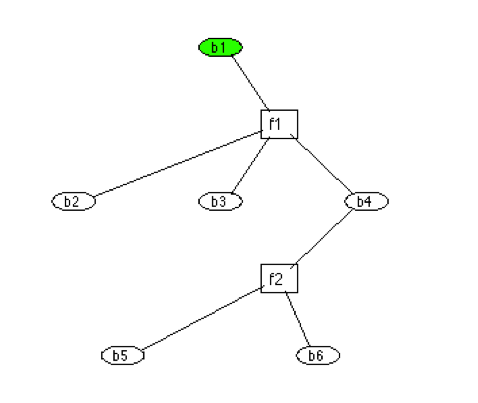
\includegraphics{images/Introspection.png}
 
As you might guess fg.depthFirstSearch(b(1),3) will return a collection of six nodes: b1, f1, b2, b3, b4, and f2.  It will not include b5 and b6 since those are at a depth of four from b1.
\fi

\ifjava
\begin{lstlisting}
FactorGraph fg = new FactorGraph();
Bit [] b = new Bit[6];
for (int i = 0; i < b.length; i++)
{
	b[i] = new Bit();
	b[i].setName("B" + i);
}
Factor f1 = fg.addFactor(new XorDelta(), b[0],b[1],b[2],b[3]);
f1.setName("f1");
Factor f2 = fg.addFactor(new XorDelta(), b[3],b[4],b[5]);
f2.setName("f2");
 
MapList<INode> nodes = fg.depthFirstSearch(b[0],3);

for (INode n : nodes)
{
	System.out.println(n);
}
\end{lstlisting}

results in:

\begin{lstlisting}
B0
f1
B1
B2
B3
f2
\end{lstlisting}
 
As you might guess fg.depthFirstSearch(b[0],3) will return a collection of six nodes: b0, f1, b1, b2, b3, and f2.  It will not include b5 and b6 since those are at a depth of four from b1.

\fi





\subsection{Variables and Related Classes}

\subsubsection{Variable Types}

The following variable types are defined in Dimple.  Some variable types are supported by only a subset of solvers.  The following table lists the Dimple variable types and the solvers that support them.

\begin{longtable} {l | p{7cm}}
Variable Type & Supported Solvers \\
\hline
\endhead
Discrete & all \\
Bit & all \\
Real & SumProduct, Gibbs, ParticleBP \\
RealJoint & SumProduct, Gibbs \\ 
Complex & SumProduct, Gibbs \\
FiniteFieldVariable & all\footnote{The performance enhanced implementations of built-in factors for FiniteField variables are only available when using the SumProduct solver.} \\
\end{longtable} 

\subsubsection{Common Properties and Methods}

The following properties and methods are common to variables of all types.

\para{Properties}

\subpara{Name}

Read-write.  When read, retrieves the current name of the variable or array of variables.  When set, modifies the name of the variable to the corresponding value.  The value set must be a string.

\ifmatlab
\begin{lstlisting}
var.Name = 'string';
\end{lstlisting}

When setting the Name, only one variable in an array may be set at a time.  To set the names of an entire array of variables to distinct values, the setNames method may be used (see section~\ref{sec:Variable.setNames}).

\fi

\ifjava
\begin{lstlisting}
var.setName('string');
\end{lstlisting}

\fi

\subpara{Label}

Read-write. All variables and factors in a Factor Graph must have unique names. However, sometimes it is desirable to have variables or factors share similar strings when being plotted or printed. Users can set the Label property to set the name for display. If the Label is not set, the Name will be used for display. Once the label is set, the label will be used for display.

\ifmatlab
\begin{lstlisting}
var.Label = 'string';
\end{lstlisting}
\fi

\ifjava
\begin{lstlisting}
var.setLabel('string');
\end{lstlisting}
\fi


\subpara{Domain}

Read-only.  Returns the domain in a form that depends on the variable type, as summarized in the following table:

\begin{longtable} {l | p{7cm}}
Variable Type & Domain Data Type \\
\hline
\endhead
Discrete & DiscreteDomain (see section~\ref{sec:DiscreteDomain}) \\
Bit & DiscreteDomain (see section~\ref{sec:DiscreteDomain}) \\
Real & RealDomain (see section~\ref{sec:RealDomain}) \\
RealJoint & RealJointDomain (see section~\ref{sec:RealJointDomain}) \\ 
Complex & ComplexDomain (see section~\ref{sec:ComplexDomain}) \\
FiniteFieldVariable & FiniteFieldDomain (see section~\ref{sec:FiniteFieldDomain}) \\
\end{longtable} 


\subpara{Solver}

Read-only.  Returns the solver-object associated with the variable, to which solver-specific methods can be called.  See section~\ref{sec:SolversAPI}, which describes the solvers, including the solver-specific methods for each solver.

\subpara{Guess}
\label{sec:Variable.Guess}

Read-write.  Specifies a value from the variable to be used when computing the Score of the factor graph (or of the variable or neighboring factors).  The Guess must be a valid value from the domain of the variable.

If the Guess had not yet been set, its value defaults to the most likely belief (which corresponds to the Value property of the variable)\footnote{For some solvers, beliefs are not supported for all variable types; in such cases there is no default value, so a Guess must be specified in order to compute the Score.}.


\subpara{Score}
\label{sec:Variable.Score}

Read-only.  When read, computes and returns the score (energy) of the Input to this variable, which is treated as a single-edge factors, given a specified value for the variable.  The score value is relative, and may be arbitrarily normalized by an additive constant.

The value of the variable used when computing the Score is the Guess value for this variable (see section~\ref{sec:Variable.Guess}).  If no Guess had yet been specified, the value with the most likely belief (which corresponds to the Value property of the variable) is used\footnote{For some solvers, beliefs are not supported for all variable types; in such cases there is no default value, so a Guess must be specified.}.


\subpara{Internal Energy}
\label{sec:Variable.InternalEnergy}

Read-only.  (Only applies to the Sum Product Solver).  When read, returns:

\[
InternalEnergy(i) = \sum_{d \in D}B_i(d)*(-log(Input(d))) 
\]

Read-only.  When read returns:

Where D is variable i's domain, Input is the variable's input, and $B_i$ is the variable Belief.

\ifjava
\begin{lstlisting}
double ie = v.getInternalEnergy();
\end{lstlisting}
\fi

\subpara{Bethe Entropy}
\label{sec:Variable.BetheEntropy}

Read-only.  (Only applies to the Sum Product Solver).  When read, returns:

\[
BetheEntropy(i) = - \sum{d \in D}B_i(d)*log(B_i(d))
\]

Where D is variable i's domain and $B_i$ is the variable Belief.

\ifjava
\begin{lstlisting}
double be = v.getBetheEntropy();
\end{lstlisting}
\fi


\subpara{Ports}

Read-only.  Retrieves \ifmatlab a cell array \fi \ifjava an array \fi containing a list of Ports connecting the variable to its neighboring factors.

\ifmatlab
\para{Methods}
\fi

\ifmatlab
\subpara{setNames}
\label{sec:Variable.setNames}

For an array of variables, the setNames method sets the name of each variable in the array to a distinct value derived from the supplied string argument.  When called with:

\begin{lstlisting}
varArray.setName('baseName');
\end{lstlisting}

the resulting variable names are of the form: \texttt{baseName\textunderscore vv0}, \texttt{baseName\textunderscore vv1}, \texttt{baseName\textunderscore vv2}, etc., where each variable's name is the concatenation of the base name with the suffix \texttt{\textunderscore vv} followed by a unique number for each variable in the array.
\fi

\ifmatlab
\subpara{invokeSolverSpecificMethod}

\begin{lstlisting}
variableArray.invokeSolverSpecificMethod('methodName', arguments);
\end{lstlisting}

For an array of variables, the invokeSolverSpecificMethod calls the specified solver-specific method on each of the variables in the array.  Here, 'methodName' is a text string with the name of the solver-specific method, and arguments is an optional comma-separated list of arguments to that method.  This method does not result in any return values.  For solver specific methods that return results, use the invokeSolverSpecificMethodWithReturnValue method instead.

\fi

\ifmatlab
\subpara{invokeSolverSpecificMethodWithReturnValue}

\begin{lstlisting}
returnArray = variableArray.invokeSolverSpecificMethodWithReturnValue('methodName', arguments);
\end{lstlisting}

For an array of variables, the invokeSolverSpecificMethodWithReturnValue calls the specified solver-specific method on each of the variables in the array, returning a return value for each variable.  Here, 'methodName' is a text string with the name of the solver-specific method, and arguments is an optional comma-separated list of arguments to that method.  The returnArray is a cell-array of the return values of the method, with dimensions equal to the dimensions of the variable array.

\fi

\ifmatlab
\para{Operators}

\subpara{Operators for Implicit Factor Creation}

Dimple supports a set of overloaded MATLAB operators and functions that operate on variables to implicitly add factors to a factor graph.

The list of supported operators and functions is given in section~\ref{sec:overloaded}.  A description of how to use these operators and functions is given in section~\ref{sec:ImplicitFactorCreation}.

Using one of the defined operators or functions with one or more variables will result in creation of a new variable, which can be assigned to a new variable name, with the appropriate domain.  It will also result in the creation of a factor which is added to the most recently created factor graph.  This factor will connect to the input variables and the newly created result variable.  For example:

\begin{lstlisting}
c = a + b;
\end{lstlisting}

This results in the creation of a Sum factor with connected variables, c, a, and b (in that order).

These operators and functions can be compounded into a single line of code, resulting in creation of intermediate anonymous variables.  For example:

\begin{lstlisting}
z = (a + b) * c^d - sqrt(-e);
\end{lstlisting}

Like using the addFactor method, some of the inputs to these operators and functions may be constants.  Specifically, for binary operators, one of the inputs may be a constant instead of a variable.  For example:

\begin{lstlisting}
x = a^2;
y = (a + b + 2) * 3;
z = a * (2 + 1i);
\end{lstlisting}

These operators and functions can be applied to arrays of variables, with some limitations.  Specifically, if each of the input variables are vectors of the same dimension, then the result will be to create a vector of output variables of the same dimension, along with a vector of factors relating the inputs and outputs.

In some cases, to be consistent with MATLAB notation, there is a distinction made between the vectorized and non-vectorized operator.  Specifically, Dimple uses MATLAB's notation for pointwise product and power operators to indicate a vectorized operation.  For example, if variables a through e are vectors of variables of identical size, then the following would create a variable vector z, and a series of factors relating these variables.

\begin{lstlisting}
z = (a .* b) + c.^d - sqrt(-e);
\end{lstlisting}

For binary operators, one of the inputs may be a scalar variable or a scalar constant instead of a variable vector.  For a scalar variable, the result is that scalar variable connecting to each instance of the factors that are created.  For a constant, each instance of the factor uses the same constant for that input (vectors of distinct constants are not currently supported).

\subpara{repmat}

Dimple overloads the MATLAB repmat function when called with a Dimple variable or variable array as its first argument.  The result of this function is an array of variables in the requested dimensions.  Dimple does not actually make multiple copies of the variables, but instead creates a variable array that provides repeated references to the same variables in the existing array.  

For example:
\begin{lstlisting}
var = Bit(10, 1);
varRef = repmat(var, 1, 10);
\end{lstlisting}

In this case varRef is a 10x10 array of variables.  Each element of varRef, however, is not a distinct Dimple variable, but a reference to an element in var, where for each row of varRef, there are 10 repeated copies of the corresponding variable in var.  Use of repmat for variables can be useful when using addFactorVectorized (see sections~\ref{sec:vectorizedFactorCreation} and~\ref{sec:FactorGraph.addFactorVectorized}).

\fi

\subsubsection{Discrete}
\label{sec:Discrete}

A Discrete variable represents a variable that can take on a finite set of distinct states.  The Discrete class corresponds to either a single Discrete variable or a multidimensional array of Discrete variables.  All properties/methods can either be called for all elements in the collection or for individual elements of the collection.

\para{Constructor}

The Discrete constructor can be used to create an N-dimensional collection of Dimple Discrete variables.  The constructor is called with the following arguments (arguments in brackets are optional).

\ifmatlab
\begin{lstlisting}
Discrete(domain, [dimensions])
\end{lstlisting}
\fi

\ifjava
\begin{lstlisting}
Discrete(domain)
\end{lstlisting}
\fi

\ifmatlab
\begin{itemize}
\item domain is a required argument indicating the domain of the variable.  The domain may either be a numeric array of domain elements, a cell array of domain elements, or a DiscreteDomain object (see section~\ref{Discrete.Domain}).
\item dimensions is an optional variable-length comma-separated list of matrix dimensions (an empty list indicates a single Discrete variable).
\end{itemize}
\fi

\ifjava
\begin{itemize}
\item domain is a required argument indicating the domain of the variable.  The domain may either be an object array of domain elements, a comma separated list, or a DiscreteDomain object (see section~\ref{Discrete.Domain}).
\end{itemize}
\fi

For example:

\ifmatlab
\begin{lstlisting}
domain = [0 1 2];
w = Discrete(domain);
x = Discrete(domain, 4);
y = Discrete(domain, 2, 3);
z = Discrete(domain, 2, 3, 4);
\end{lstlisting}
\fi

\ifjava
\begin{lstlisting}
Object [] domain = new Object [] {0,1,2};
Discrete w = new Discrete(domain);
Discrete x = new Discrete(0,1,2);
DiscreteDomain dd = DiscreteDomain.create(0,1,2);
Discrete y = new Discrete(dd);
\end{lstlisting}
\fi

We examine each of these arguments in more detail in the following sections.

\subpara{Domain}
\label{Discrete.Domain}

Every Discrete random variable has a domain associated with it.  A domain is a set.  Elements of the set may be any object type.  For example, the following are Discrete variables with valid domains:

\ifmatlab
\begin{lstlisting}
a = Discrete({1, 2, 3});
b = Discrete({1+i, i, 2*i});
c = Discrete({[1 0; 0 1], [i 1, 2*i 1]});
d = Discrete({[1 0; 0 1], 2, i+1});
e = Discrete({1.2, 3, pi/2});
f = Discrete({'red', 'green', 'blue'});
\end{lstlisting}
\fi

\ifjava
\begin{lstlisting}
Discrete a = new Discrete(1, 2, 3);
Discrete b = new Discrete(new double [] {1,0,0,1},1); 
Discrete c = new Discrete("red","blue",2);
\end{lstlisting}
\fi

\ifmatlab
(a) creates a variable whose domain consists of three values: 1, 2, and 3.  (b) creates a variable whose domain consists of three complex numbers.  (c) creates a variable whose domain consists of two elements, each of which is a 2x2 complex matrix.  (d) creates a variable whose domain consists of three elements: a matrix, real scalar, and complex scalar.  (e) creates a variable whose domain consists of both floating-point and integer values.  (f) creates a variable whose domain is a set of strings.

In the previous example we used cell arrays to specify the elements of a domain.  When the domain consists only of numeric values (integer or floating-point), domains can instead be specified as a numeric array.  In this case, each element of the array (regardless of the array's dimensions) is considered a distinct entry in the domain.

\begin{lstlisting}
a = Discrete(0:2);
b = Discrete([1 2 3; 4 5 6]);
c = Discrete([0:2]');
\end{lstlisting}

(a) creates a variable with a domain of 0, 1, and 2.  (b) creates a variable with a domain of 1, 2, 3, 4, 5, 6.  (c) creates a variable with domain of 0, 1, and 2.

\fi

The domain may also be specified using a DiscreteDomain object.  In that case, the domain of the variable consists of the elements of this object.  For example:

\ifmatlab
\begin{lstlisting}
myDomain = DiscreteDomain(0:10);
a = Discrete(myDomain);
\end{lstlisting}
\fi

\ifjava
\begin{lstlisting}
DiscreteDomain myDomain = DiscreteDomain.create(0,1,2);
Discrete a = new Discrete(myDomain);
\end{lstlisting}
\fi

See section~\ref{sec:DiscreteDomain} for more information about the DiscreteDomain class.

\ifmatlab
\subpara{List of Matrix Dimensions}
\label{sec:VariableMatrixDimensions}

If the variable constructor is called without any dimensions, a single variable will be created.

If one dimension n is specified, a square array of dimensions n x n variables will be created\footnote{This follows a common MATLAB convention.}.

With k dimensions specified, n1, n2, ..., nk, a multidimensional variable array of dimensions n1 x n2 x ... x nk will be created.

\fi

\para{Properties}

\subpara{Belief}
\label{sec:Discrete.Belief}

Read-only.  For any single variable, the Belief method returns a vector whose length is the total number of elements of the domain of the variable.  When called after running a solver to perform inference on the graph, each element of the vector contains the estimated marginal probability of the corresponding element of the domain of the variable.  The results are undefined if called prior to running a solver.

For an array of variables, the Belief method will return an array of vectors (that is, an array one dimension larger than the variable array) containing the beliefs of each variable in the array.

\subpara{Value}
\label{sec:Discrete.Value}

Read-only.  In some cases, one may wish to retrieve the single most likely element of a variable's domain.  The Value property does just that.

For any single variable, the Value method returns a single value chosen from the domain of the variable.  When called after running a solver to perform inference on the graph, the value returned corresponds to the element in the variable's domain that has the largest estimated marginal probability\footnote{If more than one domain element has identical marginal probabilities that are larger than for any other value, a single value from the domain is returned, chosen arbitrarily among these.}.  The results are undefined if called prior to running a solver.

For an array of variables, the Value method will return an array of values, each from the domain of the corresponding variable representing the largest estimated marginal probability for that variable.

\subpara{Input}
\label{sec:Discrete.Input}

Read-write.  For any variable, the Input method can be used to set and return the current input of that variable. An input behaves much like a single edge factor connected to the variable, and is typically used the represent the likelihood function associated with a measured value (see section~\ref{sec:LikelihoodInput}).

When read, for a single variable returns an array of values with each value representing the current input setting for the corresponding element of the variable's domain.  The length of this array is equal to the total number of elements of the domain.  When read, for an array of variables, the result is an array with dimension one larger than the dimension of the variable array.  The additional dimension represents the current set of input values for the corresponding variable in the array.

When written, for a single variable, the value must be an array of length equal to the domain of the variable.  The values in the array must all be non-negative, and non-infinite, but are otherwise arbitrary.  When written, for an array of variables, the values must be a multidimensional array where the first set of dimensions exactly match the dimensions of the array (or the portion of the array) being set, and length of the last dimension is the number of elements in the variable's domain.


\subpara{FixedValue}
\label{sec:Discrete.FixedValue}

Read-write.  For any variable, the FixedValue property can be used to set the variable to a specific fixed value, and to retrieve the fixed-value if one has been set.  This would generally be used for conditioning a graph on known data without modifying the graph (see section~\ref{sec:FixingAVariableValue}).

Reading this property results in an error if no fixed value has been set.  To determine if a fixed value has been set, use the hasFixedValue method (see section~\ref{sec:Discrete.hasFixedValue}).

When setting this property on a single variable, the value must be a value included in the domain of the variable.
The fixed value must be a value chosen from the domain of the variable.  For example:

\ifmatlab
\begin{lstlisting}
a = Discrete(1:10);
a.FixedValue = 3;
\end{lstlisting}
\fi

\ifjava
\begin{lstlisting}
Discrete a = new Discrete(1,2,3);
a.setFixedValue(3);
\end{lstlisting}
\fi

When setting this property on a variable array, the value must be an array of the same dimensions as the variable array, and each entry in the array must be an element of the domain.

Because the Input and FixedValue properties serve similar purposes, setting one of these overrides any previous use of the other.  Setting the Input property removes any fixed value and setting the FixedValue property replaces the input with a delta function---the value 0 except in the position corresponding to the fixed value that had been set.


\para{Methods}

\subpara{hasFixedValue}
\label{sec:Discrete.hasFixedValue}

This method takes no arguments.  When called for a single variable, it returns a boolean indicating whether or not a fixed-value is currently set for this variable.  When called for a variable array, it returns a boolean array of dimensions equal to the size of the variable array, where each entry indicates whether a fixed value is set for the corresponding variable.

\subsubsection{Bit}

A Bit is a special kind of Discrete with domain [0 1].

\para{Constructor}


\ifmatlab
The Bit constructor can be used to create an N-dimensional collection of Dimple Discrete variables.  Its constructor does not require a domain, since the domain is predetermined.  The constructor takes only a variable-length list of matrix dimensions, where an empty list indicates a single Bit variable.

\begin{lstlisting}
Bit([dimensions])
\end{lstlisting}

The behavior of the list of dimensions is identical to that for Discrete variables as described in section~\ref{sec:VariableMatrixDimensions}.

\fi

\ifjava
\begin{lstlisting}
Bit()
\end{lstlisting}
\fi

\para{Properties}

\subpara{Belief}

Read-only.  For a single Bit variable, the Belief property is a single number that represents the estimated marginal probability of the value one.

For an array of Bit variables, the Belief property is an array of numbers with size equal to the size of the variable array, with each value representing the estimated marginal probability of one for the corresponding variable.

\subpara{Value}

See section~\ref{sec:Discrete.Value}.

\subpara{Input}

Read-write.  For setting the Input property on a single Bit variable, the value must be a single number in the range 0 to 1, which represents the normalized likelihood of the value one (see section~\ref{sec:LikelihoodInput}).  If $L(x)$ is the likelihood of the variable, the Input should be set to $\frac{L(x=1)}{L(x=0) + L(x=1)}$.

For setting the Input property on an array of Bit variables, the value must be an array of normalized likelihood values, where the array dimensions must match the dimensions of the array (or the portion of the array) being set.


\subpara{FixedValue}

See section~\ref{sec:Discrete.FixedValue}.

\para{Methods}

\subpara{hasFixedValue}

See section~\ref{sec:Discrete.hasFixedValue}.


\subsubsection{Real}

A Real variable represents a variable that takes values on the real line, or on a contiguous subset of the real line.  \ifmatlab The Real class corresponds to either a single Real variable or a multidimensional array of Real variables.  All properties/methods can either be called for all elements in the collection or for individual elements of the collection.  \fi

\para{Constructor}

\ifmatlab
\begin{lstlisting}
Real([domain], [dimensions])
\end{lstlisting}
\fi

\ifjava
\begin{lstlisting}
Real()
Real(RealDomain domain)
Real(double lowerBound, double upperBound)
\end{lstlisting}
\fi

\ifmatlab
All arguments are optional and can be used in any combination.

\begin{itemize}
\item domain specifies a bound on the domain of the variable. It can either be specified as a two-element array or a RealDomain object (see section~\ref{sec:RealDomain}).  If specified as an array, the first element is the lower bound and the second element is the upper bound. -Inf and Inf are allowed values for the lower or upper bound, respectively.  If no domain is specified, then a domain from $-\infty$ to $\infty$ is assumed.
\item dimensions specify the array dimensions.  The behavior of the list of dimensions is identical to that for Discrete variables as described in section~\ref{sec:VariableMatrixDimensions}.
\end{itemize}
\fi

\ifjava
\begin{itemize}
\item domain specifies a bound on the domain of the variable. It can either be specified as two elements or a RealDomain object (see section~\ref{sec:RealDomain}).  If specified as two values, the first element is the lower bound and the second element is the upper bound. Negative infinity and positive infinity are allowed values for the lower or upper bound, respectively.  If no domain is specified, then a domain from $-\infty$ to $\infty$ is assumed.
\end{itemize}
\fi

Examples:

\ifmatlab
\begin{itemize}
\item Real() specifies a scalar real variable with an unbounded domain.
\item Real(4,1) specifies a 4x1 vector of real variables with unbounded domain.
\item Real([-1 1]) specifies a scalar real variable with domain from -1 to 1.
\item Real([-Inf 0], 4, 10, 2) specifies a 4x10x2 array of real variables, each with the domain from negative infinity to zero.
\item Real(RealDomain(-pi, pi)) specifies a scalar real variable with domain from $-\pi$ to $\pi$.
\end{itemize}
\fi

\ifjava
\begin{itemize}
\item Real() specifies a scalar real variable with an unbounded domain.
\item Real(-1, 1) specifies a scalar real variable with domain from -1 to 1.
\item Real(Double.NEGATIVE\_INFINITY,0) specifies a variable with the domain from negative infinity to zero.
\item Real(RealDomain.create(-Math.PI, Math.PI)) specifies a scalar real variable with domain from $-\pi$ to $\pi$.
\end{itemize}
\fi


\para{Properties}

\subpara{Belief}

Read-only.  The behavior of this property for Real variables is solver specific.  Some solvers do not support this property at all and will return an error when read.  See section~\ref{sec:SolversAPI} for more detail on each of the supported solvers.

For the SumProduct solver, this property returns the estimated marginal distribution of the variable in the form of a NormalParameters object (see section~\ref{sec:NormalParameters}), which includes a mean and precision value\ifmatlab\footnote{For backward compatibility with Dimple version 0.04 and earlier, the Belief can be treated as a two-dimensional array where the first element is the mean and the second is the standard deviation.}\fi.  \ifmatlab For an array of Real variables, this property returns a cell array of NormalParameters objects, each corresponding to the estimated marginal distribution of the corresponding variable. \fi The results are undefined if called prior to running a solver.


\subpara{Value}

Read-only.  The behavior of this property for Real variables is solver specific.  Some solvers do not support this property at all and will return an error when read.  See section~\ref{sec:SolversAPI} for more detail on each of the supported solvers.

For the SumProduct solver, the Value corresponds to the mean value of the belief.


\subpara{Input}

Read-write.  For a Real variable, the Input property is expressed in the form of a FactorFunction object that can connect to exactly one Real variable.  The list of available built-in FactorFunctions is given in section~\ref{sec:usingBuiltInFactors}.  Typically, an Input would use one of the standard distributions included in this list.  In this case, it must be one in which all the parameters can be fixed to pre-defined constants.  For the Gibbs and ParticleBP solvers, any such factor function may be used as an Input.  For the SumProduct solver, however, only a Normal factor function may be used.  Below is an example of setting the Input for a Real variable:

\ifmatlab

\begin{lstlisting}
r = Real();
r.Input = FactorFunction('Normal', measuredMean, measurementPrecision);
\end{lstlisting}

Equivalently, a simpler alternative form for specifying the Input may be used.  In this form the name of the factor followed by the arguments to the corresponding constructor are listed as elements of a cell array:

\begin{lstlisting}
r = Real();
r.Input = {'Normal', measuredMean, measurementPrecision};
\end{lstlisting}

To remove an Input that had previously been set, the Input may be set to an empty array.

\fi

\ifjava

\begin{lstlisting}
Real r = new Real();
r.setInput(new Normal(measuredMean, measurementPrecision));
\end{lstlisting}

To remove an Input that had previously been set, the Input may be set to null.

\fi

\ifmatlab
In the current version of Dimple, Inputs on Real variable arrays must be set one at a time, or all set to a single common value\footnote{This restriction may be removed in a future version.}.
\fi

\subpara{FixedValue}

Read-write.  The behavior of the FixedValue property for a Real variable is nearly identical to that of Discrete variables (see section~\ref{sec:Discrete.FixedValue}).  When setting the FixedValue of a Real variable, the value must be within the domain of the variable, that is greater than or equal to the lower bound and less than or equal to the upper bound.  For example:

\ifmatlab
\begin{lstlisting}
a = Real([-pi pi]);
a.FixedValue = 1.7;
\end{lstlisting}
\fi

\ifjava
\begin{lstlisting}
Real a = new Real(-Math.PI,Math.PI);
a.setFixedValue(1.7);
\end{lstlisting}
\fi

Because the Input and FixedValue properties serve similar purposes, setting one of these overrides any previous use of the other.  Setting the Input property removes any fixed value and setting the FixedValue property removes the input.


\para{Methods}

\subpara{hasFixedValue}

See section~\ref{sec:Discrete.hasFixedValue}.



\subsubsection{RealJoint}

A RealJoint variable is a tightly coupled set of real variables that are treated by a solver as a single joint variable rather than a separate collection of variables.  For example, in the SumProduct solver, the messages associated with RealJoint variables involve joint mean and covariance matrix rather than an individual mean and variance for each variable.

Like other variables, the RealJoint class can represent either a single RealJoint variable (representing a collection of real values) or an array of RealJoint variables.

\para{Constructor}

\ifmatlab
\begin{lstlisting}
RealJoint(domain, [dimensions])
RealJoint(numElements, [dimensions])
\end{lstlisting}

The arguments are defined as follows:

\begin{itemize}
\item domain specifies a bound on the domain of the variable.  It is specified by a RealJointDomain object (see section~\ref{sec:RealJointDomain}).  If no domain is specified, then an unbounded domain is assumed and numElements must be specified instead.
\item numElements specifies the number of joint real-valued elements. This argument is present only if the domain argument is not specified.
\item dimensions specify the array dimensions (the array of individual RealJoint variables).  The behavior of the list of dimensions is identical to that for Discrete variables as described in section~\ref{sec:VariableMatrixDimensions}.
\end{itemize}
\fi

\ifjava
\begin{lstlisting}
RealJoint(int size)
RealJoint(RealJointDomain domain)
\end{lstlisting}

The arguments are defined as follows:

\begin{itemize}
\item size specifies the number of joint real-valued elements.
\item domain specifies the domain of the RealJoint variable using a RealJointDomain object (see \ref{sec:RealJointDomain}).  Using this version of the constructor allows bounds to be specified in some or all dimensions of the domain.
\end{itemize}
\fi

\para{Properties}

\subpara{Belief}
\label{sec:RealJoint.Belief}

Read-only.  The behavior of this property for RealJoint variables is solver specific.  Some solvers do not support this property at all and will return an error when read.  See section~\ref{sec:SolversAPI} for more detail on each of the supported solvers.

For the SumProduct solver, this property returns the estimated marginal distribution of the variable in the form of a MultivariateNormalParameters object (see section~\ref{sec:MultivariateNormalParameters}), which includes a mean vector and covariance matrix.  \ifmatlab For an array of RealJoint variables, this property returns a cell array of MultivariateNormalParameters objects, each corresponding to the estimated marginal distribution of the corresponding variable. \fi The results are undefined if called prior to running a solver.

\subpara{Value}
\label{sec:RealJoint.Value}

Read-only.  The behavior of this property for Real variables is solver specific.  Some solvers do not support this property at all and will return an error when read.  See section~\ref{sec:SolversAPI} for more detail on each of the supported solvers.

For the SumProduct solver, this property returns the mean vector, with dimension equal to the dimension of the RealJoint variable.

\ifmatlab
For an array of RealJoint variables, this property returns an array where the initial dimensions correspond to the dimensions of the variable array (or portion of the variable array), and the final dimension corresponds to the dimension of the RealJoint variable.
\fi

\subpara{Input}
\label{sec:RealJoint.Input}

Read-write.  For a RealJoint variable, the Input property is expressed in one of two forms: either a single FactorFunction object that can connect to exactly one RealJoint variable, or a set of FactorFunction objects that can each connect to exactly one Real variable.  The latter case corresponds to a likelihood function where each dimension is independent.  The list of available built-in FactorFunctions is given in section~\ref{sec:usingBuiltInFactors}.  Typically, an Input would use one of the standard distributions included in this list.  In this case, it must be one in which all the parameters can be fixed to pre-defined constants.  For the Gibbs and ParticleBP solvers, any such factor function may be used as an Input.  For the SumProduct solver, however, only a MultvariateNormal factor function or a set of Normal factor functions may be used.

Below is an example of setting the Input for a RealJoint variable using a single multivariate factor function:

\ifmatlab

\begin{lstlisting}
r = Real();
r.Input = FactorFunction('MultivariateNormal', measuredMeanVector, measurementCovarianceMatrix);
\end{lstlisting}

Equivalently, a simpler alternative form for specifying the Input may be used.  In this form the name of the factor followed by the arguments to the corresponding constructor are listed as elements of a cell array:

\begin{lstlisting}
r = Real();
r.Input = {'MultivariateNormal', measuredMeanVector, measurementCovarianceMatrix};
\end{lstlisting}

To remove an Input that had previously been set, the Input may be set to an empty array.

\fi

\ifjava

\begin{lstlisting}
Real r = new Real();
r.setInput(new MultivariateNormal(measuredMeanVector, measurementCovarianceMatrix));
\end{lstlisting}

To remove an Input that had previously been set, the Input may be set to null.

\fi

\ifmatlab
To specify a set of univariate factor functions the value of this property must be a cell array of FactorFunction objects, one for each dimension of the RealJoint variable.
\fi
\ifjava
To specify a set of univariate factor functions the value of this property must be an array of FactorFunction objects, one for each dimension of the RealJoint variable.
\fi

\ifmatlab
In the current version of Dimple, Inputs on RealJoint variable arrays must be set one at a time, or all set to a single common value\footnote{This restriction may be removed in a future version.}.
\fi


\subpara{FixedValue}
\label{sec:RealJoint.FixedValue}

Read-write.  The behavior of the FixedValue property for a RealJoint variable is similar to that of Discrete variables (see section~\ref{sec:Discrete.FixedValue}).  When setting the FixedValue of a Real variable, the value must be within the domain of the variable.  When setting a fixed value, the value must be in an array with dimension equal to the dimension of the RealVariable.  For example:

\ifmatlab
\begin{lstlisting}
a = RealJoint(4);
a.FixedValue = [1.7, 2.0, 0, -1.2];
\end{lstlisting}
\fi

\ifjava
\begin{lstlisting}
RealJoint a = new RealJoint(4);
a.setFixedValue(new double[]{1.7, 2.0, 0, -1.2});
\end{lstlisting}
\fi

\ifmatlab
For an array of RealJoint variables, the fixed values of all variables may be set together.  In this case, the initial dimensions of the input array must equal the dimensions of the variable array (or subset of the variable array) being set, while the final dimension must equal the dimension of the RealJoint variable.
\fi

Because the Input and FixedValue properties serve similar purposes, setting one of these overrides any previous use of the other.  Setting the Input property removes any fixed value and setting the FixedValue property removes the input.


\para{Methods}

\subpara{hasFixedValue}

See section~\ref{sec:Discrete.hasFixedValue}.



\subsubsection{Complex}

Complex is a special kind of RealJoint variable with exactly two joint elements.

\ifmatlab
The behavior of all properties and methods is identical to that of RealJoint variables, with the exception of a few methods (described below), which that refer directly to complex numerical values. 
\fi
\ifjava
The behavior of all properties and methods is identical to that of RealJoint variables.
\fi

\para{Constructor}

\ifmatlab
\begin{lstlisting}
Complex([domain], [dimensions])
\end{lstlisting}

The arguments are defined as follows:

\begin{itemize}
\item domain specifies the domain of the Complex variable using a ComplexDomain object (see \ref{sec:ComplexDomain}).  If no domain is specified, then an unbounded domain is assumed.
\item dimensions specify the array dimensions (the array of individual Complex variables).  The behavior of the list of dimensions is identical to that for Discrete variables as described in section~\ref{sec:VariableMatrixDimensions}.
\end{itemize}

\fi

\ifjava
\begin{lstlisting}
Complex()
Complex(ComplexDomain domain)
\end{lstlisting}

The arguments are defined as follows:

\begin{itemize}
\item domain specifies the domain of the Complex variable using a ComplexDomain object (see \ref{sec:ComplexDomain}).  Using this version of the constructor allows bounds to be specified in some or all dimensions of the domain.
\end{itemize}
\fi

\para{Properties}

\subpara{Belief}

Read-only.  See section~\ref{sec:RealJoint.Belief}.

\subpara{Value}

\ifmatlab
Read-only.  This method behaves similarly to the Value property for a RealJoint variable, except the value returned is a single complex number.  For an array of Complex variables, each entry in the returned array is a complex number.
\fi
\ifjava
Read-only.  See section~\ref{sec:RealJoint.Value}.
\fi

\subpara{Input}

Read-write.  See section~\ref{sec:RealJoint.Input}.

\subpara{FixedValue}

\ifmatlab
Read-write.  This method behaves similarly to the FixedValue property for a RealJoint variable, except that the fixed value is a single complex number.  For an array of Complex variables, each entry in the array should be a complex number.  For example:

a = Complex();
a.FixedValue = 5 + 1i*2;
\fi
\ifjava
Read-write.  See section~\ref{sec:RealJoint.FixedValue}.
\fi

\para{Methods}

\subpara{hasFixedValue}

See section~\ref{sec:Discrete.hasFixedValue}.


\subsubsection{FiniteFieldVariable}

Dimple supports a special variable type called a FiniteFieldVariable, which represent finite fields with $N=2^{n}$ elements. These fields find frequent use in error correcting codes.  These variables are used along with certain custom factors that are implemented more efficiently for sum-product belief propagation than the alternative using discrete variables and factors implemented directly.  See section~\ref{sec:finiteFields} for more information on how these variables are used.

The behavior of all properties and methods is identical to that of Discrete variables.

\para{Constructor}

\ifmatlab
\begin{lstlisting}
FiniteFieldVariable(primitivePolynomial, [dimensions])
\end{lstlisting}
\fi

\ifjava
\begin{lstlisting}
FiniteFieldVariable(primitivePolynomial)
\end{lstlisting}
\fi

The arguments are defined as follows:

\ifmatlab
\begin{itemize}
\item primitivePolynomial the primitive polynomial of the finite field.  The format of the primitive polynomial follows the same definition used by MATLAB in the \texttt{gf} function.  See the MATLAB help on the \texttt{gf} function for more detail.
\item dimensions specify the array dimensions (the array of individual FiniteFieldVariable variables).  The behavior of the list of dimensions is identical to that for Discrete variables as described in section~\ref{sec:VariableMatrixDimensions}.
\end{itemize}
\fi

\ifjava
\begin{itemize}
\item primitivePolynomial the primitive polynomial of the finite field.  The format of the primitive polynomial follows the same definition used by MATLAB in the \texttt{gf} function.  See the MATLAB help on the \texttt{gf} function for more detail.
\end{itemize}
\fi

\subsubsection{DiscreteDomain}
\label{sec:DiscreteDomain}

The DiscreteDomain class represents a domain with a finite fixed set of elements. It is the type of Domain used
by Discrete variables. DiscreteDomain objects are immutable.

\para{Construction}


\ifmatlab
\begin{lstlisting}
DiscreteDomain(elementList)
\end{lstlisting}

The elementList argument is either a cell array or array of domain elements.  Every entry of the array or cell array is considered an element of the domain, regardless of the number of dimensions it has.  For a cell array, each object in the cell array is considered an element of the domain regardless of the object type.  For a numeric array, every entry in the array must be numeric.
\fi

\ifjava
Construction of a DiscreteDomain object is done using the static create method.

\begin{lstlisting}
DiscreteDomain.create(Object[] elementList)
\end{lstlisting}

The elementList argument is an array of domain elements.  Every entry of the array is considered an element of the domain, regardless of the number of dimensions it has.  For an array of Objects, each object in the array is considered an element of the domain regardless of the object type.  For a numeric array, every entry in the array must be numeric.
\fi

\para{Properties}

\subpara{Elements}

Read-only.  This property returns the set of elements in the discrete domain in the form of a one-dimensional \ifmatlab cell \fi array.



\subsubsection{RealDomain}
\label{sec:RealDomain}

The RealDomain class is used to refer to the domain of Real variables.

\para{Constructor}

\ifmatlab
\begin{lstlisting}
RealDomain([lowerBound, [upperBound] ])
\end{lstlisting}

\begin{itemize}
\item lowerBound indicates the lower bound of the domain.  The value must be a scalar numeric value.  It may be set to -Inf to indicate that there is no lower bound.  The default value is -Inf.
\item upperBound indicates the upper bound of the domain.  The value must be a scalar numeric value.  It may be set to Inf to indicate that there is no upper bound.  The default value is Inf.
\end{itemize}

\fi

\ifjava
Construction of a RealDomain object is done using the static create method.

\begin{lstlisting}
RealDomain.create()
RealDomain.create(lowerBound,upperBound)
\end{lstlisting}

\begin{itemize}
\item lowerBound indicates the lower bound of the domain.  The value must be a scalar numeric value.  It may be set to negative infinity to indicate that there is no lower bound.  If the create method with no arguments is used, the default lower bound is negative infinity.
\item upperBound indicates the upper bound of the domain.  The value must be a scalar numeric value.  It may be set to positive infinity to indicate that there is no upper bound.  If the create method with no arguments is used, the default upper bound is positive infinity.
\end{itemize}

\fi

\para{Properties}

\ifmatlab
\subpara{LB}
\fi
\ifjava
\subpara{LowerBound}
\fi

Read-only.  This property returns the value of the lower bound.  The default value is negative infinity.

\ifmatlab
\subpara{UB}
\fi
\ifjava
\subpara{UpperBound}
\fi

Read-only.  This property returns the value of the upper bound.  The default value is positive infinity.



\subsubsection{RealJointDomain}
\label{sec:RealJointDomain}

The RealJointDomain class is used to refer to the domain of RealJoint variables.

\para{Constructor}

\ifmatlab
\begin{lstlisting}
RealJointDomain(numDimensions);
RealJointDomain(listOfRealDomains);
RealJointDomain(numDimensions, realDomain);
\end{lstlisting}

\begin{itemize}
\item numDimensions indicates the number of dimensions in the domain of the RealJoint variable.  If the form of constructor that specifies numDimensions is called, then all dimensions are assumed to be unbounded.
\item listOfRealDomains is a comma-separated list or cell array of RealDomain objects, one for each dimension.  Each RealDomain in the list indicates the domain for the corresponding dimension of the RealJoint variable.
\item realDomain specifies a single RealDomain.  If the number of dimensions is specified along with a single RealDomain, then that RealDomain is used for each dimension of the domain of the RealJoint variable.
\end{itemize}
\fi

\ifjava
Construction of a RealJointDomain object is done using the static create method.

\begin{lstlisting}
RealJointDomain.create(int size)
RealJointDomain.create(RealDomain... domains)
RealJointDomain.create(RealDomain domain, int size)
\end{lstlisting}

\begin{itemize}
\item size indicates the number of dimensions in the domain of the RealJoint variable.  If the form of create that specifies only the size is called, then all dimensions are assumed to be unbounded.
\item domains is a list or array of RealDomain objects, one for each dimension.  Each RealDomain in the list indicates the domain of the corresponding dimension of the RealJoint variable.  The number of entries determines the number of dimensions.
\item domain indicates a single RealDomain that is to be used for all dimensions of the RealJoint variable.  In this form of create, the size must also be specified to indicate the number of dimensions of the RealJoint variable.
\end{itemize}
\fi

\para{Properties}

\ifmatlab
\subpara{NumElements}

Read-only.  Indicates the number of elements in the RealJointDomain, which corresponds to the number of dimensions of an associated RealJoint variable.
\fi

\subpara{RealDomains}

Read-only.  Returns the collection of RealDomains that correspond to each dimension of the RealJointDomain.


\ifjava
\para{Methods}

\subpara{getNumVars}

\begin{lstlisting}
domain.getNumVars();
\end{lstlisting}

Returns the number of elements in the RealJointDomain, which corresponds to the number of dimensions of an associated RealJoint variable.

\subpara{getRealDomain}

\begin{lstlisting}
domain.getRealDomain(dimensionIndex);
\end{lstlisting}

Returns the RealDomain that correspond to the dimension corresponding to the specified \texttt{dimensionIndex}.

\fi


\subsubsection{ComplexDomain}
\label{sec:ComplexDomain}

The ComplexDomain class, a subclass of the RealJointDomain class, is used to refer to the domain of Complex variables.

\para{Constructor}

\ifmatlab
\begin{lstlisting}
ComplexDomain();
ComplexDomain(listOfRealDomains);
ComplexDomain(realDomain);
\end{lstlisting}

\begin{itemize}
\item listOfRealDomains comma-separated list of exactly two RealDomain objects, one for each dimension.  Each RealDomain in the list indicates the domain for the corresponding dimension of the Complex variable (real followed by imaginary).  If no RealDomains are specified, then both dimensions are assumed to be unbounded.
\item realDomain specifies a single RealDomain to apply to both dimensions of the domain of the Complex variable.
\end{itemize}
\fi

\ifjava
Construction of a ComplexDomain object is done using the static create method.

\begin{lstlisting}
ComplexDomain.create()
ComplexDomain.create(RealDomain... domains)
ComplexDomain.create(RealDomain domain)
\end{lstlisting}

\begin{itemize}
\item domains is an array of exactly two RealDomain objects, one for each dimension.  Each RealDomain in the list indicates the domain of the corresponding dimension of the Complex variable (real followed by imaginary).  If no domains argument is specified, then both dimensions are assumed to be unbounded.
\item domain is a single RealDomain object.  When only one RealDomain object is specified, the same RealDomain is used for both dimensions.
\end{itemize}
\fi

\para{Properties}

\ifmatlab
\subpara{NumElements}

Read-only.  Indicates the number of elements in the ComplexDomain, which should always equal two.
\fi

\subpara{RealDomains}

Read-only.  Returns the collection of RealDomains that correspond to each dimension of the ComplexDomain (real followed by imaginary).


\ifjava
\para{Methods}

\subpara{getNumVars}

\begin{lstlisting}
domain.getNumVars();
\end{lstlisting}

Returns the number of elements in the ComplexDomain, which should always equal two.

\subpara{getRealDomain}

\begin{lstlisting}
domain.getRealDomain(dimensionIndex);
\end{lstlisting}

Returns the RealDomain that correspond to the dimension corresponding to the specified \texttt{dimensionIndex}.

\fi



\subsubsection{FiniteFieldDomain}
\label{sec:FiniteFieldDomain}

The FiniteFieldDomain class represents the domain of a FiniteFieldVariable.  FiniteFieldDomain objects are immutable.

\para{Construction}

\ifmatlab
\begin{lstlisting}
FiniteFieldDomain(primitivePolynomial)
\end{lstlisting}
\fi

\ifjava
Construction of a FiniteFieldDomain object is done using the static create method.

\begin{lstlisting}
FiniteFieldDomain.create(primitivePolynomial)
\end{lstlisting}
\fi

\begin{itemize}
\item primitivePolynomial is an integer representation of the primitive polynomial of the finite field.
\end{itemize}


\para{Properties}

\subpara{Elements}

Read-only.  This property returns the set of elements in the discrete domain in the form of a one-dimensional \ifmatlab cell \fi array.

\subpara{PrimitivePolynomial}

Read-only.  This property returns the primitive polynomial associated with the domain using an integer representation.

\subpara{N}

Read-only.  This property returns the number of bits in the finite field.  The size of the Elements property is $2^{N}$.




\subsubsection{NormalParameters}
\label{sec:NormalParameters}

The NormalParameters class is used to specify the parameters of a univariate Normal distribution, as used in the SumProduct solver.

\para{Constructor}

\begin{lstlisting}
NormalParameters(mean, precision)
\end{lstlisting}

\begin{itemize}
\item mean is the mean value of the distribution.
\item precision is the precision of the distribution, which is the inverse of the variance.
\end{itemize}


\para{Properties}

\subpara{Mean}

Read-only.  Returns the mean value.

\subpara{Precision}

Read-only.  Returns the precision value.

\subpara{Variance}

Read-only.  Returns the variance (inverse of the precision).

\subpara{StandardDeviation}

Read-only.  Returns the standard deviation (square root of the variance).




\subsubsection{MultivariateNormalParameters}
\label{sec:MultivariateNormalParameters}

The MultivariateNormalParameters class is used to specify the parameters of a multivariate Normal distribution, as used in the SumProduct solver.

\para{Constructor}

\begin{lstlisting}
MultivariateNormalParameters(meanVector, covarianceMatrix)
\end{lstlisting}

\begin{itemize}
\item meanVector indicates the mean value of each element in a joint set of variables.  The value must be a one-dimensional numeric array.
\item covarianceMatrix indicates the covariance matrix associated with the elements of a joint set of variables.  The value must be a two-dimensional numeric array with each dimension identical to the length of the meanVector.
\end{itemize}


\para{Properties}

\subpara{Mean}

Read-only.  Returns a vector of values, where each value indicates the mean value of the corresponding element in a joint set of variables.

\subpara{Covariance}

Read-only.  Returns a two-dimensional array of values, representing the covariance matrix of a joint set of variables.

\subpara{InformationVector}

Read-only.  Returns a vector of values representing the information matrix, defined as $\Sigma^{-1}\mu$, where $\Sigma$ is the covariance matrix and $\mu$ is the mean vector.

\subpara{InformationMatrix}

Read-only.  Returns a two-dimensional array of values representing the information matrix, defined as $\Sigma^{-1}$, where $\Sigma$ is the covariance matrix.






\subsection{Factors and Related Classes}

\subsubsection{Factor}

The Factor class can represent either a single factor or a multidimensional array of factors.  The Factor class is never created directly, but is the result of using the addFactor or addFactorVectorized (or related) methods on a FactorGraph.

\para{Properties}

\subpara{Name}

Read-write.  When read, retrieves the current name of the factor or array of factors.  When set, modifies the name of the factor to the corresponding value.  The value set must be a string.

\ifmatlab
\begin{lstlisting}
factor.Name = 'string';
\end{lstlisting}

When setting the Name, only one factor in an array may be set at a time.  To set the names of an entire array of factors to distinct values, the setNames method may be used (see section~\ref{sec:Factor.setNames}).

\fi

\ifjava
\begin{lstlisting}
factor.setName("string");
\end{lstlisting}
\fi


\subpara{Label}

Read-write. All variables and factors in a Factor Graph must have unique names. However, sometimes its desirable to have variables or factors share similar strings when being plotted or printed. Users can set the Label property to set the name for display. If the Label is not set, the Name will be used for display. Once the label is set, the label will be used for display.

\ifmatlab
\begin{lstlisting}
factor.Label = 'string';
\end{lstlisting}
\fi

\ifmatlab
\begin{lstlisting}
factor.setLabel("string");
\end{lstlisting}
\fi


\subpara{DirectedTo}
\label{sec:Factor.DirectedTo}

\ifmatlab
Read-write.  The DirectedTo property indicates a set of variables to which the factor is directed.  The value may be either a single variable or a cell array of variables.  The DirectedTo property is used by some solvers, and in some cases is required for proper operation of certain features.  Such cases are identified elsewhere in this manual.
\fi

\ifjava
Read-write.  The DirectedTo property indicates a set of variables to which the factor is directed.  The value may be either a single variable, a comma separated list of variables, a VariableList, or an array of integers specifying the edge indexes to which the factor is directed.  The DirectedTo property is used by some solvers, and in some cases is required for proper operation of certain features.  Such cases are identified elsewhere in this manual.
\fi

For example, if a factor F corresponds to a function $F(a, b, c, d)$, where $a$, $b$, $c$, and $d$ are variables, then the factor is directed toward $c$ and $d$ if $\sum_{c, d} F(a, b, c, d)$ is constant for all values of $a$ and $b$.  In this case, we may set:

\ifmatlab
\begin{lstlisting}
F.DirectedTo = {c, d};
\end{lstlisting}
\fi

\ifjava
\begin{lstlisting}
F.setDirectedTo(c,d);
\end{lstlisting}
\fi

In some cases, the set of DirectedTo variables can be automatically determined when a factor is created.  In this case it need not be set manually by the user.  This includes many built-in factors supported by Dimple.  If this property is set by the user, then in the case of factors connected only to discrete variables, Dimple will check that the factor is in fact directed in the specified direction.

\ifmatlab
If the set of variables the factor are directed toward are part of a variable array, then these may be specified together in a single cell array.  For example, if varArray is an array of variables, and a factor F is directed toward all of the variables in varArray, then we can set:

\begin{lstlisting}
F.DirectedTo = varArray;
\end{lstlisting}

In the case of a vector of factors, we can identify the variables to which each factor is directed in a vectorized way.  For example:

\begin{lstlisting}
s = Discrete(domain,N);
fg.addFactorVectorized(factorFunction, s(1:(end-1)), s(2:end)).DirectedTo = s(2:end);
\end{lstlisting}

This example also shows that the DirectedTo property can be set directly on the result of the factor creation without assigning the factor to a named variable.

As a more complicated vectorized example, the following creates 12 factors, each of which contains 10 variables (5 from a and 5 from b).  The first 2 of the 5 from a and the first from b are what the factor is directed to.

\begin{lstlisting}
a = Bit(3,4,5);
b = Bit(3,4,5);
fg.addFactorVectorized(factorFunction, {a, [1 2]}, {b, [1 2]}).DirectedTo = {a(:,:,1:2), b(:,:,1)};
\end{lstlisting}
\fi

\subpara{Score}
\label{sec:Factor.Score}

Read-only.  When read, computes and returns the score (energy) of the factor given a specified value for each of the neighboring variables to this factor.  The score represents the energy of the factor given the specified variable configuration.  The score value is relative, and may be arbitrarily normalized by an additive constant.

The value of each variable used when computing the Score is the Guess value for that variable (see section~\ref{sec:Variable.Guess}).  If no Guess had yet been specified for a given variable, the value with the most likely belief (which corresponds to the Value property of the variable) is used\footnote{For some solvers, beliefs are not supported for all variable types; in such cases there is no default value, so a Guess must be specified.}.

The variable energy is normalized by the maximum input probability.

\subpara{InternalEnergy}
\label{sec:Factor.InternalEnergy}

Read-only.  (Only applies to the Sum Product Solver).  When read returns:

\[
InternalEnergy(a) = \sum_{\vec{x} \in \vec{X}}B_a(\vec{x})*(-log(Weight(\vec{x})))
\]

Where a is an instance of a Factor, X is the set of variables connected to a, Weight is the FactorTable entry for the specified set of variable values, and $B_a$ is the belief of that factor node.

\ifjava
\begin{lstlisting}
double ie = f.getInternalEnergy();
\end{lstlisting}
\fi

\subpara{Bethe Entropy}
\label{sec:Factor.BetheEntropy}

Read-only.  (Only applies to the Sum Product Solver).  When read returns:

\[
BetheEntropy(a) = - \sum_{\vec{x} \in domain(\vec{X})}B_a(\vec{x})*log(B_a(\vec{x})) 
\]

Where a is an instance of a Factor, X is the set of variables connected to a, and $B_a$ is the belief of that factor node.
\ifmatlab
\begin{lstlisting}
double be = f.getBetheEntropy();
\end{lstlisting}
\fi

\subpara{Belief}
\label{sec:Factor.Belief}

Read-only.  (Only applies to the Sum Product Solver). To support the Bethe Free Energy property, Dimple provides getBelief associated with a Factor.

\[
Belief_a(\vec{x}) = Weight(\vec{x})\prod_{i=0}^N \mu_{X_i \rightarrow a}(x_i)
\]

Where $ \vec{x} \in domain(\vec{X}) $ and $ \vec{X} $ is the set of variables connected to the factor a.

\ifmatlab
\begin{lstlisting}
b = f.Belief;
\end{lstlisting}
\fi
\ifjava
\begin{lstlisting}
double b = f.getBelief();
\end{lstlisting}
\fi


\subpara{Ports}

Read-only.  Retrieves \ifmatlab a cell array \fi \ifjava an array \fi containing a list of Ports connecting the factor to its neighboring variables.


\ifmatlab
\para{Methods}

\subpara{setNames}
\label{sec:Factor.setNames}

For an array of factors, the setNames method sets the name of each factor in the array to a distinct value derived from the supplied string argument.  When called with:

\begin{lstlisting}
factorArray.setName('baseName');
\end{lstlisting}

the resulting factor names are of the form: \texttt{baseName\textunderscore vv0}, \texttt{baseName\textunderscore vv1}, \texttt{baseName\textunderscore vv2}, etc., where each factor's name is the concatenation of the base name with the suffix \texttt{\textunderscore vv} followed by a unique number for each factor in the array.


\subpara{invokeSolverSpecificMethod}

\begin{lstlisting}
factorArray.invokeSolverSpecificMethod('methodName', arguments);
\end{lstlisting}

For an array of factors, the invokeSolverSpecificMethod calls the specified solver-specific method on each of the factors in the array.  Here, 'methodName' is a text string with the name of the solver-specific method, and arguments is an optional comma-separated list of arguments to that method.  This method does not result in any return values.  For solver specific methods that return results, use the invokeSolverSpecificMethodWithReturnValue method instead.


\subpara{invokeSolverSpecificMethodWithReturnValue}

\begin{lstlisting}
returnArray = factorArray.invokeSolverSpecificMethodWithReturnValue('methodName', arguments);
\end{lstlisting}

For an array of factors, the invokeSolverSpecificMethodWithReturnValue calls the specified solver-specific method on each of the factors in the array, returning a return value for each variable.  Here, 'methodName' is a text string with the name of the solver-specific method, and arguments is an optional comma-separated list of arguments to that method.  The returnArray is a cell-array of the return values of the method, with dimensions equal to the dimensions of the factor array.

\fi

\subsubsection{DiscreteFactor}

When all variables connected to a Factor are discrete, a DiscreteFactor is created.

\para{Properties}

\subpara{Belief}
\label{sec:Factor.Belief}

Read-only.  The belief of a factor is the joint belief over all joint states of the variables connected to that factor.  There are two properties that represent the belief in different ways: Belief and FullBelief.  Reading the Belief property after the solver has been run\footnote{In the current version of Dimple, the Belief property is only supported for factors connected exclusively to discrete variables, and is supported only by the SumProduct solver.  These restrictions may be removed in a future version.} returns the belief in a compact one-dimensional vector that includes only values that correspond to non-zero entries in the factor table.  This form is used because in some situation, the full representation over all possible variable values (as returned by the FullBelief property) would result in a data structure too large to be practical.

\ifmatlab
\begin{lstlisting}
fb = myFactor.Belief;
\end{lstlisting}
\fi

\ifjava
\begin{lstlisting}
double [] fb = myFactor.getBelief();
\end{lstlisting}
\fi

The result is a vector of belief values, where the order of the vector corresponds to the order of the factor table entries.  The order of factor table entries can be determined from the factor using:

\ifmatlab
\begin{lstlisting}
ind = f.FactorTable.Indices
\end{lstlisting}
\fi

\ifjava
\begin{lstlisting}
int [][] indices = f.getFactorTable().getIndices()
\end{lstlisting}
\fi

This returns a two-dimensional array, where each row corresponds to one entry in the factor table, and where each column-entry in a row indicates the index into the domain of the corresponding variable (where the order of the variable is the order used when the factor was created).


\subpara{FullBelief}
\label{sec:Factor.FullBelief}

Read-only.  Reading the FullBelief property after the solver has been run\footnote{In the current version of Dimple, the Belief property is only supported for factors connected exclusively to discrete variables, and is supported only by the SumProduct solver.  These restrictions may be removed in a future version.} returns the belief in a multi-dimensional array, where each dimension of the multi-dimensional array ranges over the domain of the corresponding variable (the order of the dimensions corresponds to the variable order used when the factor was created).

\ifmatlab
\begin{lstlisting}
fb = myFactor.FullBelief;
\end{lstlisting}
\fi

\ifjava
\begin{lstlisting}
double [] fb = myFactor.getFullBelief();
\end{lstlisting}
\fi

\subsubsection{FactorFunction}
\label{sec:FactorFunction}

\ifmatlab

The FactorFunction class is used to specify a Dimple built-in factor function in a way that can be reused for creating multiple factors, and that allows specification of constructor arguments.

\para{Constructor}

\begin{lstlisting}
FactorFunction(factorFunctionName, [constructorArguments])
\end{lstlisting}

\begin{itemize}
\item factorFunctionName is a string that indicates the name of the built-in factor function.
\item constructorArguments is a variable-length comma-separated list of constructor arguments, whose interpretation is specific to the particular built-in factor function.  If no arguments are needed, this list would be empty.
\end{itemize}

There are no available properties or methods in this class.

\fi

\ifjava
The FactorFunction class is an abstract class that is used as the base class for all FactorFunctions passed to the addFactor call.  To create new FactorFunctions, users must override the FactorFunction class.

\para{Constructors}

\begin{itemize}
\item FactorFunction()
\item FactorFunction(String name);
\end{itemize}

\para{Methods}

At least one or the other of these must be overridden in a derived class.  Users should override evalEnergy instead of eval, but for now can override one or the other.  Eventually eval should be made final and so that only evalEnergy can be overridden.

\begin{itemize}
\item double eval(Object ... args) - Should return a probability associated with the passed in configuration of arguments.
\item double evalEnergy(Object ... args) - Should return -log(probability) associated with the passed in configuration of arguments.
\end{itemize}

\fi

\subsubsection{FactorTable}
\label{sec:FactorTable}

The FactorTable class is used to explicitly specify a factor table in lieu of Dimple creating one automatically from a factor function.  This is sometimes useful in cases where the factor table is highly structured, but automatic creation would be time consuming due to a large number of possible states of the connected variables.

\para{Constructor}

\ifmatlab
\begin{lstlisting}
FactorTable([ ( indexList, weightList ) | weightMatrix ], domains)
\end{lstlisting}

A FactorTable is constructed by specifying the table values in one of two forms, or by creating an all-zeros FactorTable to be filled in later using the set method.  The first form, specifying an indexList and weightList, is useful for sparse factor tables in which many entires are zero and need not be included in the table.  The second form, specifying a weightMatrix, is useful for dense factor tables in which most or all of the entries are non-zero.


\begin{itemize}
\item indexList is an array where each row represents a set of zero-based indices into the list of domain elements for each successive domain in the given set of domains.
\item weightList is a one-dimensional array of real-valued entries in the factor table, where each entry corresponds to the indices given by the corresponding row of the indexList.
\item weightMatrix is an N dimensional array of real-valued entries in the factor table.  The number of dimensions, N, must correspond to the number of discrete domain elements given in the subsequent arguments, and the number of elements in each dimension must equal the number of elements in the corresponding domain element.
\item domains is a comma-separated list of one or more discrete variable domains.  Each domain either in the form of a DiscreteDomain object or a cell-array of the elements of the domain.  From an existing variable, the domain can be obtained using the Domain property of that variable.
\end{itemize}

An example using the first method is:
\begin{lstlisting}
a = Bit;
b = Bit;
c = Bit;
ft = FactorTable([0 0 0; 0 1 1; 1 0 1; 1 1 0], [1 .9 .5 .3], a.Domain, b.Domain, c.Domain);
\end{lstlisting}

An example using the second method is:
\begin{lstlisting}
a = Discrete({'red','green','blue'});
b = Bit;
ft = FactorTable([.5 .4; .3 .1; 0 .4], a.Domain, b.Domain);
\end{lstlisting}

\fi

\ifjava

\begin{itemize}
\item FactorTable.create(DiscreteDomain ... domains) - Creates a full table with with the specified domains.
\item FactorTable.create(int [][] indices, double [] weights,DiscreteDomain ... domains) - Creates a table with the specified indices and weights with the specified domains
\item FactorTable.create(int [][] indices, double [] weights, Discrete ... variables) - Same as the previous method but extracts the domains from the variables.
\item FactorTable.create(Object table, DiscreteDomain [] domains) - Assumes table is a tensor (number of dimensions equal to number of domains).  
\end{itemize}

A FactorTable is constructed by specifying the table values in one of two forms, or by creating an all-zeros FactorTable to be filled in later using the set method.  The first form, specifying an indexList and weightList, is useful for sparse factor tables in which many entires are zero and need not be included in the table.  The second form, specifying a weightMatrix, is useful for dense factor tables in which most or all of the entries are non-zero.

\begin{itemize}
\item indices is an array where each row represents a set of zero-based indices into the list of domain elements for each successive domain in the given set of domains.
\item weights is a one-dimensional array of real-valued entries in the factor table, where each entry corresponds to the indices given by the corresponding row of the indexList.
\item table is an N dimensional array of real-valued entries in the factor table.  The number of dimensions, N, must correspond to the number of discrete domain elements given in the subsequent arguments, and the number of elements in each dimension must equal the number of elements in the corresponding domain element.
\end{itemize}

\fi

\para{Properties}

\subpara{Indices}

Read-write.  When read, returns an array of indices of the factor table corresponding to entries in the factor table.  Each row represents a set of zero-based indices into the list of domain elements for each successive domain in the given set of domains.

When written, replaces the previous array of indices with a new array.  When writing using this property, the number of rows in the table must not change since this must equal the number of entires in the Weights.  To change both Indices and Weights simultaneously, use the change method.

\subpara{Weights}

Read-write.  When read, returns a one-dimensional array of real-valued entries in the factor table, where each entry corresponds to the indices given by the corresponding row of the indexList.

When written, replaces the previous array of weights.  When writing using this property, the number of entries must not change since this must equal the number of rows in the Indices.  To change both Indices and Weights simultaneously, use the change method.

\subpara{Domains}

Read-only.  Returns \ifmatlab a cell-array \fi \ifjava an array \fi of DiscreteDomain objects, each of which represents the corresponding domain specified in the constructor, in the same order as specified in the constructor.


\para{Methods}

\subpara{set}
\label{sec:FactorTable.set}


\ifmatlab

This method allows setting individual entries in the factor table.  For each entry to be set, the domain values (not indices) are specified followed by the weight value.  To set a single entry, the domain values are specified in a comma-separated list, followed by the weight value.  To set multiple entries in a single call, a cell array of such comma-separated lists are specified.

An example of setting a single entry:
\begin{lstlisting}
ft.set('red', 1, 0.45);
\end{lstlisting}

An example of setting multiple entries:
\begin{lstlisting}
ft.set({'red', 1, 0.45}, {'blue', 0, 0.75});
\end{lstlisting}
\fi

\ifjava

This method allows setting individual entries in the factor table.  For each entry to be set, the indices are specified followed by the weight value.  

\begin{lstlisting}
ft.set(new int [] {0,1,1},1.0);
\end{lstlisting}
\fi

\subpara{get}

\ifmatlab
This method retrieves the weight associated with a particular entry in the factor table.  The entry is specified by a comma-separated list of domain values (not indices).  For example:

\begin{lstlisting}
w = ft.get('red', 1);
\end{lstlisting}
\fi

\ifjava
This method retrieves the weight associated with a particular entry in the factor table.  The entry is specified by a comma-separated list of indices.  For example:

\begin{lstlisting}
double w = ft.get(new int [] {0,1,1});
\end{lstlisting}
\fi

\subpara{change}

This method allows simultaneously replacing both the array of Indices and Weights in the factor table.

\begin{lstlisting}
ft.change(indexList, weightList);
\end{lstlisting}

The arguments indexList and weightList are exactly as described in the FactorTable constructor.


\subsection{Schedulers}
\label{sec:Schedulers}

A scheduler defines a rule that determines the update schedule of a factor graph when performing inference.  This section describes all of the built-in schedulers available in Dimple.

Each scheduler is applicable only to a certain subset of solvers.  For all of the BP solvers (SumProduct, MinSum, Gaussian, ParticleBP), the following schedulers are available:

\begin{longtable}{l p{4in}}
\textbf{Name} & \textbf{Description} \\ \hline \hline
%
\textsf{DefaultScheduler} & Same as the TreeOrFloodingScheduler, which is the default if no scheduler or custom schedule is specified. \\ \hline
%
\textsf{TreeOrFloodingScheduler} & The solver will use either a Tree Schedule or a Flooding Schedule depending on whether the factor-graph contains cycles.  In a nested graph, this choice is applied independently in each subgraph.  If the factor-graph is a tree, the scheduler will automatically detect this and use a Tree Schedule.  In this schedule, each node is updated in an order that will result in the correct beliefs being computed after just one iteration.  If the entire graph is a tree, NumIterations should be set to 1, which is its default value.  If the factor-graph is loopy, the solver will instead use a Flooding Schedule (as described below). \\ \hline
%
\textsf{TreeOrSequentialScheduler} & The solver will use either a Tree Schedule (as described above) or a Sequential Schedule (as described below) depending on whether the factor-graph contains cycles.  In a nested graph, this choice is applied independently in each subgraph.  \\ \hline
%
\textsf{FloodingScheduler} & The solver will apply a Flooding Schedule.  For each iteration, all variable nodes are updated, followed by all factor nodes.  Because the graph is bipartite (factor nodes only connect to variable nodes, and vice versa), the order of update within each node type does not affect the result. \\ \hline
%
\textsf{SequentialScheduler} & The solver will apply a Sequential Schedule.  For each factor node in the graph, first, for each variable connected to that factor, the edge connecting the variable to the factor is updated; then the factor node is updated.  The specific order of factors chosen is arbitrary, and depends on the order that factors were added to the graph. \\ \hline
%
\textsf{RandomWithoutReplacementScheduler} & The solver will apply a Sequential Schedule with the order of factors chosen randomly without replacement.  On each subsequent iteration, a new random order is chosen.  Since the factor order is chosen randomly with replacement, on each iteration, each factor will be updated exactly once. \\ \hline
%
\textsf{RandomWithReplacementScheduler} & The solver will apply a Sequential Schedule with the order of factors chosen randomly with replacement.  On each subsequent iteration, a new random order is chosen.  The number of factors updated per iteration is equal to the total number of factors in the graph. However, since the factors are chosen randomly with replacement, not all factors are necessarily updated in a single iteration, and some may be updated more than once. \\ \hline
%
\end{longtable}


In a nested graph, for most of the schedulers listed above (except for the random schedulers), the schedule is applied hierarchically.  In particular, a subgraph is treated as a factor in the nesting level that it appears.  When that subgraph is updated, the schedule for the corresponding subgraph is run in its entirety, updating all factors and variables contained within according to its specified schedule.

It is possible for subgraphs to be designated to use a schedule different from that of its parent graph.  This can be done by specifying either a scheduler or a custom schedule for the subgraph prior to adding it to the parent graph.  For example:

\ifmatlab
\begin{lstlisting}
SubGraph.Scheduler = 'SequentialScheduler';
ParentGraph.addFactor(SubGraph, boundaryVariables);
ParentGraph.Scheduler = 'FloodingScheduler';
\end{lstlisting}
\fi

\ifjava
\begin{lstlisting}
SubGraph.setScheduler(new com.analog.lyric.dimple.schedulers.SequentialScheduler()); 
ParentGraph.addFactor(SubGraph , a,b); 
ParentGraph.setScheduler(new com.analog.lyric.dimple.schedulers.TreeOrFloodingScheduler());		
\end{lstlisting}
\fi

For the TreeOrFloodingScheduler and the TreeOrSequentialScheduler, the choice of schedule is done independently in the outer graph and in each subgraph.  In case that a subgraph is a tree, the tree scheduler will be applied when updating that subgraph even if the parent graph is loopy.  This structure can improve the performance of belief propagation by ensuring that the effect of variables at the boundary of the subgraph fully propagates to all other variables in the subgraph on each iteration.

For the RandomWithoutReplacementScheduler and RandomWithReplacementScheduler, if these are applied to a graph or subgraph, the hierarchy of any lower nesting layers is ignored.  That is, the subgraphs below are essentially flattened prior to schedule creation, and any schedulers or custom schedules specified in lower layers of the hierarchy are ignored.


Because of the differences in operation between the Gibbs solver and the BP based solvers, the Gibbs solver supports a distinct set of schedulers.  For the Gibbs solver, the following schedulers are available:

\begin{tabular}{l p{4in}}
\textbf{Name} & \textbf{Description} \\ \hline \hline
%
\textsf{GibbsDefaultScheduler} & Same as the GibbsSequentialScanScheduler, which is the default when using the Gibbs solver. \\ \hline
%
\textsf{GibbsSequentialScanScheduler} & The solver will apply a Sequential Scan Schedule.  For each scan, each variable is resampled in a fixed order.  The specific order of variables chosen is arbitrary, and depends on the order that variables were added to the graph. \\ \hline
%
\textsf{GibbsRandomScanScheduler} & The solver will apply a Random Scan Schedule.  Each successive variable to be resampled is chosen randomly with replacement.  The number of variables resampled per scan is equal to the total number of variables in the graph, but not all variables are necessarily resampled in a given scan, and some may be resampled more than once. \\ \hline
%
\end{tabular}

Because of the nature of the Gibbs solver, the nested structure of a graph is ignored in creating the schedule.  That is, the graph hierarchy is essentially flattened prior to schedule creation, and only the scheduler specified on the outermost graph is applied.

Schedulers are not applicable in the case of the LP solver.


\subsection{Solvers}
\label{sec:SolversAPI}

% TODO: make a separate file for each solver

\subsubsection{Solver-Specific Options}

Each solver supports a number of options specific to that solver. These are described in the following sections. Solver-specific options may be used to configure how overall inference works for that solver or may be used to configure the behavior of individual factors or variables for that solver. Solver-specific options are typically set on the applicable model object (factor graph, factor, or variable) and the values will be observed and used to configure the corresponding solver objects:

\ifmatlab
\begin{lstlisting}
%*\textit{model-object}*.setOption('%*\textit{SolverOptionClass.optionName}*', %*\textit{option-value}*)
\end{lstlisting}
\fi
\ifjava
\begin{lstlisting}
%*\textit{model-object}*.setOption(%*\textit{SolverOptionClass.optionName}*, %*\textit{option-value}*)
\end{lstlisting}
\fi

Solver-specific options may be set at any time, even before the solver for a graph has been specified.  Options that are not applicable to the object on which it is set or that are not applicable to the active solver will simply be ignored.  For more details on the options mechanism see \autoref{sec:Options} of this document.

\subsubsection{Solver-Specific Methods}

Each solver also may support solver-specific methods, which are described in the following sections. As with options, solver-specific methods may be available for various objects: a factor-graph, variable, or factor. In each case, to call a solver-specific method, the method is applied to the solver object, returned by the Solver property.  For example:

\ifmatlab
\begin{lstlisting}
factorGraph.Solver.%*\textit{solverSpecificMethod}*(arguments);
\end{lstlisting}

\begin{lstlisting}
variable.Solver.%*\textit{solverSpecificMethod}*(arguments);
\end{lstlisting}

\begin{lstlisting}
factor.Solver.%*\textit{solverSpecificMethod}*(arguments);
\end{lstlisting}
\fi

\ifjava
\begin{lstlisting}
((%*\textit{SolverSpecificGraph}*)fg.getSolver()).%*\textit{solverSpecificMethod}*(arguments);
\end{lstlisting}

\begin{lstlisting}
((%*\textit{SolverSpecificVar}*)variable.getSolver()).%*\textit{solverSpecificMethod}*(arguments);
\end{lstlisting}

\begin{lstlisting}
((%*\textit{SolverSpecificFactor}*)factor.getSolver()).%*\textit{solverSpecificMethod}*(arguments);
\end{lstlisting}

The downcast in the first cast can be avoided if you save the return value from \lstname{setSolverFactory} and call the methods through that. For example:

\begin{lstlisting}
JunctionTreeSolverGraph sgraph =
    fg.setSolverFactory(new JunctionTreeSolver());
sgraph.useConditioning(true);
\end{lstlisting}

The downcasts are also not required for common methods available to all solvers described in the next section.
\fi

Some solver-specific methods return results, while others do not.  Some solver-specific methods require arguments, while others do not.  \ifmatlab If no arguments are needed, the parentheses are optional. \fi

\ifmatlab

In some cases it is convenient to call solver-specific methods on each element in an array of objects.  Utility methods are provided for this purpose.  Specifically, to call a solver-specific method that has no return value:
\begin{lstlisting}
objectArray.invokeSolverSpecificMethod('methodName', arguments);
\end{lstlisting}

In this case, 'methodName' is a text string with the name of the solver-specific method, and arguments is an optional comma-separated list of arguments to that method.

To call a solver specific method that has a return value:
\begin{lstlisting}
returnArray = objectArray.invokeSolverSpecificMethodWithReturnValue('methodName', arguments);
\end{lstlisting}

In this case, returnArray is a cell-array of the return values of the method, with dimensions equal to the dimensions of the object array.

\fi

\subsubsection{Common Options}

A few options are applicable to multiple solvers and are therefore described in this subsection.

\para{SolverOptions.enableMultithreading}

\dimpleOption{SolverOptions.enableMultithreading}
{boolean}
{false}
{graph}
{Controls whether to use multithreading for this solver. Multithreading is currently only supported by the MinSum and SumProduct solvers but will eventually be implemented in others. This value will be ignored if not applicable.}

\para{SolverOptions.maxAutomaticFactorTableSize}

\dimpleOption{SolverOptions.maxAutomaticFactorTableSize}
{32-bit integer}
{max signed value: $2^{31} - 1$}
{discrete factor}
{This controls whether factor tables will be automatically computed at initialization time for discrete factors based on the expected number of entries in the table. Factor table creation can be expensive both in the memory it takes to store large tables and in the time that is needed to evaluate the factor function for every possible combination of arguments. This option provides a means to set a threshold for creation.
\linebreak
\linebreak
The expected size of the table is computed differently based on whether the factor is directed and the function is deterministic:
\begin{itemize}
\item If the factor is not deterministic directed, then the expected size of the factor table is the sizes of all of the variable domains multiplied together.
\item If the factor is deterministic and directed the expected size, then the expected size is the sizes of just the input variable domains multipled together.
\end{itemize}

This will not prevent factor tables from being generated manually. Only applicable to discrete factors, and currently only useful when using the Gibbs solver.}

\para{DimpleOptions.randomSeed}

\dimpleOption{DimpleOptions.randomSeed}
{64-bit integer}
{N/A}
{graph}
{When set, this option specifies a random seed that may be used by solvers that use a random number generator. The seed will only be used if explicitly set; the default value is not used. This can be used to ensure repeatable behavior during testing or profiling but should not be used for normal operation.}

\subsubsection{Common Methods}

There are also some methods that are common to all solvers. These are:

\para{getMultithreadingManager}

Dimple users can retrieve a MultithreadingManager on which to perform additional actions.

\ifmatlab
\begin{lstlisting}
fg.Solver.getMultithreadingManager()
\end{lstlisting}
\fi

\ifjava
\begin{lstlisting}
fg.getSolver().getMultithreadingManager()
\end{lstlisting}
\fi

Users can configure both the multithreading mode and the number of workers using the MultithreadingManager.

\subparagraph{Multithreading Modes}

Dimple provides various multithreading algorithms that have different speed advantages depending on the size of the user's graph and FactorTables.  In the future Dimple should be modified to automatically detect the best threading algorithm.  Currently, however, it defaults to the "Phase" multithreading mode and requires the user manually set the mode to change this.  For a given graph, users can try both modes and see which is faster.

The currently supported multithreading modes are:

\begin{itemize}
\item Phase - Divides the schedule into "phases" where each phase contains schedule entries that are entirely independent of one another.  These phases are then easy to parallelize.  
\item SingleQueue - Uses a single queue and a dependency graph to pull off work for each thread on the fly.  
\end{itemize}

The following methods can be used for getting and setting modes:


\ifmatlab

\begin{itemize}
\item fg.Solver.getMultithreadingManager().getModes() - Returns a Java array of enums specifying the valid modes.
\item fg.Solver.getMultithreadingManager().setMode(ModeName) - Allows users to set the mode by string.  Currently "Phase" or "SingleQueue" will work.
\item fg.Solver.getMultithreadingManager().setMode(enum) - Allows users to set the mode by the enums returned by the getModes method.
\end{itemize}

\fi

\ifjava
\begin{itemize}
\item fg.getSolver().getMultithreadingManager().getModes() - Returns an array of enums specifying the valid modes.
\item fg.getSolver().getMultithreadingManager().setMode(ModeName) - Allows users to set the mode by string.  Currently "Phase" or "SingleQueue" will work.
\item fg.getSolver().getMultithreadingManager().setMode(enum) - Allows users to set the mode by the enums returned by the getModes method or with MultithreadingMode.<PhaseName>.
\end{itemize}
\fi

\subparagraph{Setting Number of Threads and Workers}

Dimple provides a ThreadingPool as a singleton for multithreading.  It sets the number of threads in this pool to the number of virtual cores in the user's machine by default.  Users can override this default value.  In addition, Dimple allows users to specify the number of "workers" for a given FactorGraph.  This "NumWorkers" is also set to the number of virtual cores on the user's machine by default.  Whereas NumThreads specifies how many threads are in the threadPool, NumWorkers specifies how work is divided up across the graph.  These workers are run by the thread pool.  Best performance is achieved when NumWorkers and NumThreads are the same.  However, NumThreads is global and shared by all graphs where NumWorkers is specific to a given FactorGraph.

The following methods can be used to change number of workers:

\ifjava
\begin{itemize}
\item fg.getSolver().getMultithreadingManager().getNumWorkers()
\item fg.getSolver().getMultithreadingManager().setNumWorkers(num)
\item fg.getSolver().getMultithreadingManager().setNumWorkersToDefault()
\end{itemize}
\fi

\ifmatlab
\begin{itemize}
\item fg.Solver.getMultithreadingManager().getNumWorkers()
\item fg.Solver.getMultithreadingManager().setNumWorkers(num)
\item fg.Solver.getMultithreadingManager().setNumWorkersToDefault()
\end{itemize}
\fi

The following global methods can be used to set the number of threads in the ThreadPool

\ifmatlab
\begin{itemize}
\item getDimpleNumThreads()
\item setDimpleNumThreads(numThreads)
\item setDimpleNumThreadsToDefault()
\end{itemize}
\fi

\ifjava
\begin{itemize}
\item ThreadPool.getNumThreads()
\item ThreadPool.setNumThreads(numThreads)
\item ThreadPool.setNumThreadsToDefault()
\end{itemize}
\fi

\clearpage
\subsubsection{Common Belief Propagation Options}
\label{sec:BPOptions}

There are a number of options that are applicable to multiple solvers that are based on some form of message-passing belief propagation. These include the Sum-Product, Min-Sum, Particle BP, and Junction Tree solvers. These options are defined in the BPOptions class. The following options are supported:

\para{BPOptions.iterations}

\dimpleOption{BPOptions.iterations}
{integer}
{1}
{graph}
{Controls how many iterations to perform when running solve(). This is not applicable to all solvers. It is currently only used by the SumProduct, MinSum and ParticleBP solvers. It only makes sense to set this to a value greater than one if the graph is not singly connected or "loopy", that is when there is more than one unique path between two or more nodes in the graph. You can tell if a graph is loopy using the FactorGraph method isForest(), which will be false if the graph is not singly connected.}

\para{BPOptions.scheduler}

\dimpleOption{BPOptions.scheduler}
{scheduler}
{DefaultScheduler}
{graph}
{Controls what scheduling strategy will be used for ordering edge updates. The option may either be specified as an actual scheduler object or as the name or instance of the scheduler class.}

\para{BPOptions.scheduleValidator}

\dimpleOption{BPOptions.scheduleValidator}
{string}
{AllEdgeScheduleValidator}
{graph}
{Specifies validation strategy for schedules. This is used to validate schedules produced by CustomScheduler. The default validator ensures that the schedule contains at least one edge entry for each direction of every edge in the graph. The NullScheduleValidator may be used to disable validation of custom schedules.}

\para{BPOptions.damping}

\dimpleOption{BPOptions.damping}
{double}
{0.0}
{variables and factors}
{The belief propogation based solvers supports damping, in which messages are damped by replacing each message by a weighted sum of the computed message value and the previous value of that message (when the corresponding edge was most-recently updated). In the current version of Dimple, damping is supported only in discrete variables and factors that connect only to discrete variables\footnote{Support for damping for continuous variables may be added in a future release.}.
\linebreak
\linebreak
The damping parameter specifies a weighting value in the range 0 through 1:

\[
\mathrm{message} = \mathrm{computedMessage} \cdot (1 - D) + \mathrm{previousMessage} \cdot D
\]

where $D$ is the damping value. So that a value of 0 means that the previous message will not be considered, effectively turning off damping.
\linebreak
\linebreak
This option applies the same damping parameter to all edges connected to the variable or factor on which it is set. If you want different values for different edges, you need to use the \nameref{option:BPOptions.nodeSpecificDamping} option.
}

\para{BPOptions.nodeSpecificDamping}

\dimpleOption{BPOptions.nodeSpecificDamping}
{\ifmatlab double vector\fi \ifjava OptionDoubleList\fi}
{\textit{empty}}
{variables and factors}
{This is the similar to the \nameref{option:BPOptions.damping} option but allows you specify different weights for different edges. Unlike the simple damping option, this usually makes no sense to set on the graph itself since factors and variables will typically have different numbers and arrangements of edges. The value must either be an empty list, indicating that damping should be turned off, or a list of weights with the same length as the number of siblings of the affected variable and factor. The damping weights will be applied in the order in which the siblings are declared.
\linebreak
\linebreak
This option takes precedence over the simple damping option if both are specified for the same node.
}

\para{BPOptions.maxMessageSize}

\dimpleOption{BPOptions.maxMessageSize}
{integer}
{integer max}
{discrete factors}
{This specifies the maximum size of the outgoing messages on the discrete factors on which it is set. If this number K is less than the full size of the message (i.e. the size of the domain of the target variable), then only the K-best values -- those with the largest weights -- will be included in the message. This can results in a faster but more approximate form of inference and is most suited to graphs with very large-dimension variables.
\linebreak
\linebreak
IMPORTANT: k-best and damping are not compatible with each other\footnote{This restriction may be removed in a future version of Dimple.}}

\para{BPOptions.updateApproach}

\dimpleOption{BPOptions.updateApproach}
{\ifmatlab string\fi \ifjava UpdateApproach enum\fi}
{AUTOMATIC}
{discrete factors}
{This option controls which update algorithm is applied to discrete factors. The option can take one of three values:
\begin{itemize}
\item NORMAL - Perform updates using just the factor tables. Do not use the optimized update technique.
\item OPTIMIZED - Use the optimized update algorithm. Note that factors that have only one edge, or factors that do not have all of their edges updated simultaneously by the schedule, ignore this setting and use the normal approach.
\item AUTOMATIC - Automatically determine whether to use the optimized algorithm. The automatic selection algorithm can be tuned through the \nameref{option:BPOptions.automaticExecutionTimeScalingFactor} and \nameref{option:BPOptions.automaticMemoryAllocationScalingFactor} options.
\end{itemize}
}

\para{BPOptions.automaticExecutionTimeScalingFactor}

\dimpleOption{BPOptions.automaticExecutionTimeScalingFactor}
{double}
{1.0}
{discrete factors}
{This option is an execution time scaling factor used when the \nameref{option:BPOptions.updateApproach} option is set to AUTOMATIC. It controls how execution time costs are weighed. The value must be a positive number.}

\para{BPOptions.automaticMemoryAllocationScalingFactor}

\dimpleOption{BPOptions.automaticMemoryAllocationScalingFactor}
{double}
{10.0}
{discrete factors}
{This option is an memory allocation scaling factor used when the \nameref{option:BPOptions.updateApproach} option is set to AUTOMATIC. It controls how memory allocation costs are weighed. The value must be a positive number.}

\para{BPOptions.optimizedUpdateSparseThreshold}

\dimpleOption{BPOptions.optimizedUpdateSparseThreshold}
{double}
{1.0}
{discrete factors}
{This option controls the representation of the auxiliary tables used by the optimized update algorithm, which is controlled through the \nameref{option:BPOptions.updateApproach}. Internally, the optimized algorithm creates multiple factor tables to perform the update. This option specifies a density, below which an auxiliary table uses a sparse representation. It must be a number in the range [0.0, 1.0]. The value 1.0 (the default), indicates that a sparse representation should be used if there are any zero-entries in the table. The value 0.0 will prevent the sparse representation from being used entirely. Sparse tables typically decrease execution time, but they use more memory. When the update approach is set to AUTOMATIC, this option impacts both the execution time and memory allocation estimates used to choose the update approach.}

\clearpage
\subsubsection{Sum-Product Solver}
\label{sec:SumProductSolver}

Use of the sum-product solver is specified by calling:

\ifmatlab
\begin{lstlisting}
fg.Solver = 'SumProduct';
\end{lstlisting}
\fi

\ifjava
\begin{lstlisting}
SumProductSolverGraph sfg = fg.setSolverFactory(new SumProductSolver());
\end{lstlisting}
\fi

If no solver is specified, the SumProduct solver is used by default.

The SumProduct solver supports both discrete and continuous variables.  The SumProduct solver uses the sum-product form of belief propagation to perform inference on a graph.  For discrete variables, each message to or from a factor is in the form of a vector of length equal to the domain size of the variable.  For continuous variables, messages are represented using a Gaussian parameterization.  In some cases, this is an approximation to the exact message.  For Real variables, a message is in the form of a pair of values representing the mean and variance of the corresponding Normal distribution.  For Complex and RealJoint variables, a message is in the form of a vector and matrix, representing the mean and covariance of the corresponding multivariate Normal distribution.

While the Gaussian representation of messages for continuous variables is sometimes an approximation, there are some specific built-in factors for which exact Gaussian messages are computed.  This can be done when a factor preserves the Gaussian form of the distribution on each edge.  The following table is a list of such lists built-in factors.  See section~\ref{sec:builtInFactors} for more information on built-in factors.

\begin{longtable} {p{3.5cm} p{3.0cm} p{7.0cm}}
Built-in Factor & Variable Types &  Notes \\
\hline
\endhead
Normal & Real & Applies only if mean and precision parameters are constants and all connected variables are Real and unbounded\footnote{Unbounded means that the domain of the variable must not have finite upper or lower bounds}. \\
MultivariateNormal & Complex or \newline RealJoint & All connected variables must be RealJoint or Complex and unbounded. \\
Sum & Real & All connected variables must be Real and unbounded.  \\
Subtract & Real & All connected variables must be Real and unbounded. \\
Negate & Real & All connected variables must be Real and unbounded. \\
ComplexSum & Complex & All connected variables must be Complex and unbounded. \\
ComplexSubtract & Complex & All connected variables must be Complex and unbounded. \\
ComplexNegate & Complex & All connected variables must be Complex and unbounded. \\
RealJointSum & RealJoint & All connected variables must be RealJoint of the same dimension and unbounded. \\
RealJointSubtract & RealJoint & All connected variables must be RealJoint of the same dimension and unbounded. \\
RealJointNegate & RealJoint & All connected variables must be RealJoint of the same dimension and unbounded. \\
Product & Real, Constant & Applies only if the product is one unbounded Real variable times one scalar constant to produce an unbounded Real variable. \\
MatrixRealJoint\newline VectorProduct & RealJoint, \newline Constant & Applies only if the product is one unbounded RealJoint variable times a constant matrix to produce an unbounded RealJoint variable. \\
LinearEquation & Real & Linear equation.  All connected variables must be Real and unbounded. \\
\end{longtable}

For factors that are neither discrete-only or listed in the above table, an approximate computation is used in computing messages from such a factor.  This includes any factor that connects to both discrete and continuous variables as well as factors that connect only to continuous variables but do not appear in the list above.  The approximate method is sample based and uses Gibbs sampling to sample from the factor, allowing approximate messages to be computed from the sample statistics.  Several methods described below allow control over the behavior of these sampled factors.

For discrete-only factors, two factor update algorithms are available: normal and optimized. The optimized algorithm can be applied only to factors with more than one edge, and only when the schedule updates all of the factor's edges simultaneously. The optimized algorithm computes the outbound message update with fewer operations than the normal algorithm, which can decrease execution time; however, it also uses more memory and increases initialization time. Several options, described below, influence which algorithm is used. Key among them is the updateApproach option, which can be set to normal, optimized, or automatic. When set to automatic, Dimple makes an estimate of the memory usage and execution time of each algorithm in order to select one.


\para{GibbsOptions for Sampled Factors}

Factors connected to continuous variables that do not support exact message computation, instead use a sampled approximation (see section~\ref{sec:SumProductSolver}) where the sampling is performed using the Gibbs solver.

For all such factors in a graph, you may set any of the Gibbs solver options described in \autoref{sec:GibbsOptions} to control how the sampling will be done. The most important of these options have different default values when used with Sum-Product. This is accomplished by setting the options on the solver graph object when it is constructed. In order to override these defaults, it is necessary to set them on the solver graph (to apply to all such factors, using \texttt{graph.Solver.setOption(...))}, or on the factor specific factor object (to apply to a single factor, using \texttt{factor.setOption(...))}.

These options and their SumProduct-specific default values are:

\begin{itemize}
\item \nameref{option:GibbsOptions.numSamples}: 1000 \ifjava (See SampledFactor.DEFAULT\_SAMPLES\_PER\_UPDATE)\fi
\item \nameref{option:GibbsOptions.burnInScans}: 10 \ifjava (See SampledFactor.DEFAULT\_BURN\_IN\_SCANS\_PER\_UPDATE)\fi
\item \nameref{option:GibbsOptions.scansPerSample}: 1 \ifjava (See SampledFactor.DEFAULT\_SCANS\_PER\_SAMPLE)\fi
\end{itemize}

\clearpage
\subsubsection{Min-Sum Solver}

Use of the MinSum solver is specified by calling:

\ifmatlab
\begin{lstlisting}
fg.Solver = 'MinSum';
\end{lstlisting}
\fi

\ifjava
\begin{lstlisting}
SFactorGraph sgraph = fg.setSolverFactory(new MinSumSolver());
\end{lstlisting}
\fi

Unlike the Sum-Product solver, the Min-Sum solver supports only discrete variables. It only
uses the standard BP Options described in \nameref{sec:BPOptions}.

\clearpage
\subsubsection{Junction Tree Solver}
\label{sec:JunctionTreeSolverAPI}

There are two distinct forms of Junction Tree solver in Dimple: the sum-product form used for computing exact marginal variable beliefs and the min-sum form used for computing MAP values.  The Junction Tree solvers support only discrete variables.

Use of one of the two forms of Junction Tree solver by calling either:

\ifmatlab
\begin{lstlisting}
fg.Solver = 'JunctionTree';
\end{lstlisting}
\fi

\ifjava
\begin{lstlisting}
JunctionTreeSolverGraph sgraph =
    fg.setSolverFactory(new JunctionTreeSolver());
\end{lstlisting}
\fi

for the sum-product version or

\ifmatlab
\begin{lstlisting}
fg.Solver = 'JunctionTreeMAP';
\end{lstlisting}
\fi

\ifjava
\begin{lstlisting}
JunctionTreeMAPSolverGraph sgraph =
    fg.setSolverFactory(new JunctionTreeMAPSolver());
\end{lstlisting}
\fi

for the min-sum version.

The Junction Tree solvers are useful for performing exact inference on loopy discrete graphical models for which the standard sum-product or min-sum algorithms will only produce approximate results. This works by transforming the model into a corresponding non-loopy model, building a proxy solver layer that connects the original model to the transformed version and doing inference on that model. If your model already is non-loopy then you can simply use sum-product or min-sum directly for exact inference. To test to see if a graph is loopy or not, use \lstname{isForest()}:

\ifmatlab
\begin{lstlisting}
useJunctionTree = ~fg.isForest();
\end{lstlisting}
\fi

\ifjava
\begin{lstlisting}
useJunctionTree = !fg.isForest();
\end{lstlisting}
\fi

One significant limitation when using this solver is that the cost of inference and amount of memory needed to store the factor tables is proportional to the size of the tables, which in turn is exponential in the number of variables represented in a table. The Junction Tree algorithm may be unable to determine an equivalent tree structure that has small enough factors either to fit in memory or to perform inference on in an acceptable amount of time. The typical failure mode in such cases is to get an \lstname{OutOfMemoryError} when attempting to run solve. The Junction Tree algorithm works best when used with smaller graphs or larger graphs that have few loops or are loopy but long and narrow.

\para{Junction Tree Options}
\label{sec:JunctionTreeOptions}

The following options are available for use with both versions of the Junction Tree solver.

Because exact inference can be done in a single iteration, the Junction Tree solver fixes the number of iterations to one and will ignore attempts to set it to another value. Because damping would result in inexact inference, the Junction Tree solver does not provide options for using damping.

\subpara{JunctionTreeOptions.useConditioning}

\dimpleOption{JunctionTreeOptions.useConditioning}
{boolean}
{false}
{graph}
{Specifies whether to use conditioning when constructing the transformation of the model. When true, then any variables in the model that have a fixed value will be disconnected from the rest of the graph in the transformed version and its value will be incorporated in the factors of the transformed model. This will produce a more efficient transformed model when there are fixed values in the original model. Using this will require that a new transformation be computed every time a fixed value changes.}

\subpara{JunctionTreeOptions.maxTransformationAttempts}

\dimpleOption{JunctionTreeOptions.maxTransformationAttempts}
{integer}
{1}
{graph}
{Specifies the maximum number of times the junction tree transformer should try to determine an optimal transformation. Each attempt uses a greedy "variable elimination" algorithm using a randomly chosen cost function and random choices to break ties, so more iterations could produce a more efficient tree transformation.}


\clearpage
\subsubsection{Gibbs Solver}
\label{sec:GibbsSolverAPI}

Use of the Gibbs solver is specified by calling:

\ifmatlab
\begin{lstlisting}
fg.Solver = 'Gibbs';
\end{lstlisting}
\fi


\ifjava
\begin{lstlisting}
GibbsSolverGraph sfg = fg.setSolverFactory(new GibbsSolver());
\end{lstlisting}
\fi

The Gibbs solver supports both discrete and continuous variables.

This solver performs Gibbs sampling on a factor graph.  It supports a variety of output information on the sampled graph, including the best joint sample (lowest energy), marginals of each variable (discrete variables only), and a full set of samples for a user-selected set of variables.  The solver supports both sequential and randomized scan, and it supports tempering with an exponential annealing schedule.

The Gibbs solver supports several user selectable generic samplers (those that don't require specific conjugacy relationships).  The following table lists the available generic samplers, and the variable types supported by each.

\begin{longtable} {l l p{8.0cm}}
Sampler & Variable Type &  Description \\
\hline
\endhead
CDFSampler & Discrete\footnote{In this table, Discrete support implies any of the discrete variable types, including Discrete and Bit.} & Samples from the full conditional distribution of the variable.  This is the default sampler for discrete variables. \\
SliceSampler & Real\footnote{In this table, Real support implies any of the continuous variable data types, including Real, Complex, and RealJoint.} & Slice sampler using the doubling procedure.  See Neal, Slice Sampling (2000).  This is the default sampler for real variables. \\
MHSampler & Discrete \& Real & Metropolis-Hastings sampler.  For discrete variables, the default proposal kernel is uniform over values other than the current value.  For real variables, the default proposal kernel is Normal with standard deviation 1 (the standard deviation is user settable).  Alternate proposal kernels are also available (see below). \\
SuwaTodoSampler & Discrete & Suwa-Todo sampler.  See Suwa, Todo, Markov Chain Monte Carlo Method without Detailed Balance (2010). \\
BlockMHSampler & Discrete \& Real & Block Metropolis-Hastings sampler.  Allows block proposals for a collection of more than one variable at a time.  In the current version of Dimple, there are no built-in general purpose block proposal kernels.  To use this sampler, a custom block proposal kernel must be written in Java, and used by specifying a block schedule entry that references this proposal kernel.  See section~\ref{sec:BlockScheduleEntries} for more information.
\end{longtable}


In cases where the factors of the graph support a conjugate distribution, the solver will automatically determine this and use the appropriate conjugate sampler.  The following table lists the supported conjugate samplers and the corresponding factors that support them.  The corresponding sampler will be used for a given variable if all of the edges connected to that variable support the same sampler\footnote{Additionally, for the conjugate sampler to be used, the domain of the variable must not be bounded to a range smaller than the natural range of the corresponding distribution.}.

\begin{longtable} {l p{7.1cm} p{2.5cm}}
Sampler & Built-in Factor & Edge \\
\hline
\endhead
BetaSampler & Beta & value \\
 & Binomial & $\rho$ \\
DirichletSampler & Dirichlet & value \\
 & Categorical & $\alpha$ \\
 & DiscreteTransition & $\alpha$ \\
GammaSampler & Gamma & value, $\beta$ \\
 & NegativeExpGamma & $\beta$ \\
 & Normal & $\tau$ \\
 & LogNormal & $\tau$ \\
 & Poisson & $\lambda$ \\
 & CategoricalUnnormalizedParameters & $\alpha$ \\
 & DiscreteTransitionUnnormalizedParameters & $\alpha$ \\
NegativeExpGammaSampler & NegativeExpGamma & value \\
 & CategoricalEnergyParameters & $\alpha$ \\ 
 & DiscreteTransitionEnergyParameters & $\alpha$ \\ 
NormalSampler & Normal & value, $\mu$ \\
 & LogNormal & $\mu$ \\
\end{longtable}

Additionally, conjugate sampling is supported across a subset of applicable deterministic functions.  In the current version of Dimple, this includes the following factors:

\begin{longtable} {l p{2cm} p{9cm}}
Factor Function & Edges & Condition \\
\hline
\endhead
Multiplexer & in, out & If any of the \emph{in} variables would support the same conjugate sampler as the \emph{out} variable, then those \emph{in} variables will use conjugate sampling. \\
\end{longtable}


The Gibbs solver automatically performs block-Gibbs updates for variables that are deterministically related.  The Gibbs solver automatically detects deterministic relationships associated with built-in deterministic factor functions (see section~\ref{sec:builtInFactors} for a list of these functions).  

\ifmatlab
For user-defined factors specified by MATLAB factor functions or factor tables, the Gibbs solver will detect if they are deterministic functions as along as the factor is marked as the directed outputs are indicated using the DirectedTo property, as described in section~\ref{sec:Factor.DirectedTo}.
\fi

\ifjava
For user-defined factors specified by factor functions or factor tables, the Gibbs solver will detect if they are deterministic functions as along as the factor is marked as the directed outputs are indicated using the DirectedTo property, as described in section~\ref{sec:Factor.DirectedTo}.
\fi
 
The Gibbs solver also automatically performs block-Gibbs updates for certain built-in factors that Gibbs sampling on individual variables would fail due to the dependencies between variables imposed by the factor.  In these cases, a custom proposal distribution ensures that proposals are consistent with the constraints of the factor.  However, the custom proposals are not assured to result in efficient mixing.  In the current version of Dimple, the following built-in factors automatically implement block-Gibbs updates:
%
\begin{itemize}
\item Multinomial
\item MultinomialUnnormalizedParameters
\item MultinomialEnergyParameters
\end{itemize}


Most Dimple methods work more-or-less as normal when using the Gibbs solver, but in some cases the interpretation is slightly different than for other solvers. For example, the .Belief method for a discrete variable returns an estimate of the belief based on averaging over the sample values.

NOTE: The setNumIterations() method is not supported by the Gibbs solver as the term ``iteration'' is ambiguous in this case. Instead, the method setNumSamples() should be used to set the length of the run. The Solver.iterate() method performs a single-variable update in the case of the Gibbs solver, rather than an entire scan of all variables.

The following sections list the solver-specific aspects of the API for the Gibbs solver.

\para{Gibbs Options}
\label{sec:GibbsOptions}

The following options affect the behavior of various aspects of the Gibbs solver:

\subpara{SolverOptions.maxAutomaticFactorTableSize}

See description in \autoref{option:SolverOptions.maxAutomaticFactorTableSize}.

\subpara{GibbsOptions.numSamples}

\dimpleOption{GibbsOptions.numSamples}
{integer}
{1}
{graph}
{Specifies the number of samples to be generated when solving the graph post burn-in.  (This value times the value of \nameref{option:GibbsOptions.numRandomRestarts} plus one determines the total number of samples that will be produced.)}

\subpara{GibbsOptions.scansPerSample}

\dimpleOption{GibbsOptions.scansPerSample}
{integer}
{0}
{graph}
{Specifies sampling rate in terms of the number of scans\footnote{A scan is a number of updates to each variable equal to the number of variables in the graph.  For a fixed schedule, this typically means updating each variable exactly once.  For a random update schedule, this is not necessarily the case.} of the graph to perform for each sample.}


\subpara{GibbsOptions.burnInScans}

\dimpleOption{GibbsOptions.burnInScans}
{integer}
{0}
{graph}
{Specifies the number of scans of the graph to perform during the burn-in phase before generating samples.}

\subpara{GibbsOptions.numRandomRestarts}

\dimpleOption{GibbsOptions.numRandomRestarts}
{integer}
{0}
{graph}
{Specifies the number of random restarts (zero by default, which means run once and don't restart). For a value greater than zero, the after running the specified number of samples, the solver is restarted with the variable values randomized, and re-run (including burn-in).  The sample values (the best sample value, or all samples, if requested) are extracted across all runs.
}

\subpara{GibbsOptions.saveAllSamples}

\dimpleOption{GibbsOptions.saveAllSamples}
{boolean}
{false}
{graph}
{Specifies whether to save all sample values for variables when running Gibbs. Note that this is practical only if the number of variables in the graph times the number of samples per variable is reasonably sized.}

\subpara{GibbsOptions.saveAllScores}

\dimpleOption{GibbsOptions.saveAllScores}
{boolean}
{false}
{graph}
{Specifies whether to save scores for all generated samples in Gibbs. If true, then for each sample the total energy/log-likelihood a.k.a. \emph{score} of the graph will be saved. The saved scores can later be retrieved by the getAllScores() method described below.}

\subpara{GibbsOptions.scheduler}

\dimpleOption{GibbsOptions.scheduler}
{scheduler}
{GobbsDefaultScheduler}
{graph}
{Controls what scheduling strategy will be used for ordering variable updates. The option may either be specified as an actual scheduler object or as the name or instance of the scheduler class.}

\subpara{GibbsOptions.scheduleValidator}

\dimpleOption{GibbsOptions.scheduleValidator}
{string}
{VariablesOnlyScheduleValidator}
{graph}
{Specifies validation strategy for schedules. This is used to validate schedules produced by CustomScheduler. The default validator ensures that the schedule contains at least one node entry for every variable in the graph. The NullScheduleValidator may be used to disable validation of custom schedules.}

\subpara{GibbsOptions.discreteSampler}

\dimpleOption{GibbsOptions.discreteSampler}
{\ifmatlab string\fi \ifjava IGenericSampler class\fi}
{CDFSampler}
{variables}
{Specifies the default sampler to use for discrete variables when a conjugate sampler is not  suitable. The sampler may be configured by use of additional options defined by each sampler type. See \autoref{sec:Samplers} for more details.}

\subpara{GibbsOptions.realSampler}

\dimpleOption{GibbsOptions.realSampler}
{\ifmatlab string\fi \ifjava IGenericSampler class\fi}
{SliceSampler}
{variables}
{Specifies the default sampler to use for real-valued variables (including Complex and RealJoint) when a conjugate sampler is not suitable. The sampler may be configured by use of additional options defined by each sampler type. See \autoref{sec:Samplers} for more details.}

\subpara{GibbsOptions.enableAutomaticConjugateSampling}

\dimpleOption{GibbsOptions.enableAutomaticConjugateSampling}
{boolean}
{true}
{variables}
{Specifies whether to use conjugate sampling when available for a given variable. Note that if a specific sampler has been specified for a particular variable (by setting the \nameref{option:GibbsOptions.realSampler} option directly on the model or solver variable object) then a conjugate sampler will not be used regardless.}

\subpara{GibbsOptions.computeRealJointBeliefMoments}

\dimpleOption{GibbsOptions.computeRealJointBeliefMoments}
{boolean}
{false}
{variables}
{Specifies whether to compute the belief moments (mean vector and covariance matrix) for RealJoint (and Complex) variables while sampling.  To minimize computation, these are not computed by default for RealJoint variables (Real variables always compute similar statistics, and do not have a corresponding option to enable them).  If true, the belief moments are computed for each sample on-the-fly (without saving all samples).  The computed moments can later be retrieved by the getSampleMean and getSampleCovariance solver-specific methods for the variable (see section~\ref{sec:RealJointVariableSpecificMethods})}



\subpara{GibbsOptions.enableAnnealing}

\dimpleOption{GibbsOptions.enableAnnealing}
{boolean}
{false}
{graph}
{Specifies whether to use a tempering and annealing process when running Gibbs.}

\subpara{GibbsOptions.annealingHalfLife}

\dimpleOption{GibbsOptions.annealingHalfLife}
{double}
{1.0}
{graph}
{Specifies the rate at which the temperature will be lowered during the tempering and annealing process. This rate is specified in terms of the number of samples required for the temperature to be lowered by half. This value is only used if annealing has been enabled as specified by the enableAnnealing option.}

\subpara{GibbsOptions.initialTemperature}

\dimpleOption{GibbsOptions.initialTemperature}
{double}
{1.0}
{graph}
{Specifies the initial temperature to use when annealing is enabled (as specified by the enableAnnealing option).}


\para{Graph Methods}

The following methods are available on a graph set to use the Gibbs solver:

Variable initialization (both on the first run and subsequent restarts) is randomized whenever possible.  For a discrete variable, the value is sampled from the Input (uniform if an input is not specified).  For a real variable, if an Input is specified and the Input supports one of the conjugate samplers listed above, that sampler is used to initialize the variable.  If bounds are also specified for the variable domain, the values is truncated to fall within the bounds.  If only bounds are specified (which are finite above and below), then the value is uniformly sampled from within the bounds.  If no finite bounds are specified and there is no input, the variable is initialized to zero (or the value specified by setInitialSampleValue) on the initial run, and left at the final value of the previous run on restart.

Enable or disable the use of tempering, or determine if tempering is in use.

\ifmatlab
\begin{lstlisting}
graph.Solver.setTemperature(T);
graph.Solver.getTemperature();
\end{lstlisting}
\fi

\ifjava
\begin{lstlisting}
sfg.setTemperature(T);
sfg.getTemperature();
\end{lstlisting}
\fi

Set/get the current temperature. Setting the current temperature overrides the current annealing temperature.

\ifmatlab
\begin{lstlisting}
graph.Solver.getAllScores();
\end{lstlisting}
\fi

\ifjava
\begin{lstlisting}
sfg.getAllScores();
\end{lstlisting}
\fi

Returns an array including the score value for each sample. This method only returns a non-empty value if the \nameref{option:GibbsOptions.saveAllScores} option was set to true on the graph before generating samples.

\ifmatlab
\begin{lstlisting}
graph.Solver.getTotalPotential();
\end{lstlisting}
\fi

\ifjava
\begin{lstlisting}
sfg.getTotalPotential();
\end{lstlisting}
\fi

After running the solver, returns the total potential (score) over all factors of the graph (including input priors on variables) given the most recent sample values.

\ifmatlab
\begin{lstlisting}
graph.Solver.sample(numSamples)
\end{lstlisting}
\fi

\ifjava
\begin{lstlisting}
sfg.sample(numSamples)
\end{lstlisting}
\fi

This method runs a specified number of samples without re-initializing, burn-in, or random-restarts (this is distinct from iterate(), which runs a specified number of single-variable updates).  Before running this method for the first time, the graph must be initialized using the initialize() method.

\ifmatlab
\begin{lstlisting}
graph.Solver.burnIn()
\end{lstlisting}
\fi

\ifjava
\begin{lstlisting}
sfg.burnIn()
\end{lstlisting}
\fi

Run the burn-in samples independently of using solve (which automatically runs the burn-in samples).  This may be run before using sample() or iterate().

\ifmatlab
\begin{lstlisting}
graph.Solver.getRejectionRate()
\end{lstlisting}
\fi

\ifjava
\begin{lstlisting}
sfg.getRejectionRate()
\end{lstlisting}
\fi

Get the overall rejection rate over the entire graph.  The rejection rate is the ratio of the number of MCMC proposals that were rejected to the total number of sampler updates.  Rejections only occur in MCMC samplers, such as the MHSampler.  In other samplers, such as conjugate samplers or the CDFSampler, rejection doesn't occur and the rate for variables that use these samplers is zero (in these cases, sampling the same value twice in a row is not considered rejection).  When getting the rejection rate for the entire graph, both the number of rejections and number of updates is counted for all variables, as well as all blocks of variables over which a block sampler is used.  These counts are accumulated from the time the graph is initialized, which automatically occurs when running solve().  This includes both burn-in and subsequent sampling.  These counts can also be reset explicitly using the resetRejectionRateStats method (see below), which allows these values to be determined, for example, during a specific set of samples.

\ifmatlab
\begin{lstlisting}
graph.Solver.resetRejectionRateStats()
\end{lstlisting}
\fi

\ifjava
\begin{lstlisting}
sfg.resetRejectionRateStats()
\end{lstlisting}
\fi

Explicitly reset the rejection-rate statistics.  These are automatically reset when the graph is initialized, which automatically occurs when running solve(), but may be reset manually at other times using this method.


\para{Variable Methods}

\ifmatlab
\begin{lstlisting}
variable.Solver.getCurrentSample();
\end{lstlisting}
\fi

\ifjava
\begin{lstlisting}
Object d = ((GibbsDiscrete)variable.getSolver()).getCurrentSample();
double r = ((GibbsReal)variable.getSolver()).getCurrentSample();
double[] rj = ((GibbsRealJoint)variable.getSolver()).getCurrentSample();
Value val= ((ISolverVariableGibss)variable.getSolver()).getCurrentSampleValue();
\end{lstlisting}
\fi

Returns the current sample value for a variable.

\ifmatlab
\begin{lstlisting}
variable.Solver.getAllSamples();
\end{lstlisting}
\fi

\ifjava
\begin{lstlisting}
Object[] ds = ((GibbsDiscrete)variable.getSolver()).getAllSamples();
double[] rs = ((GibbsReal)variable.getSolver()).getAllSamples();
double[][] rjs = ((GibbsRealJoint)variable.getSolver()).getAllSamples();
\end{lstlisting}
\fi

Returns an array including all sample values seen so far for a variable. Over multiple variables, samples with the same index correspond to the same joint sample value. This method only returns a non-empty value if the \nameref{option:GibbsOptions.saveAllSamples} options was enabled for the variable when sampling was performed.

\ifmatlab
\begin{lstlisting}
variable.Solver.getBestSample();
\end{lstlisting}
\fi

\ifjava
\begin{lstlisting}
Object d = ((GibbsDiscrete)variable.getSolver()).getBestSample();
double r = ((GibbsReal)variable.getSolver()).getBestSample();
double[] rj = ((GibbsRealJoint)variable.getSolver()).getBestSample();
\end{lstlisting}
\fi


Returns the value of the best sample value seen so far, where best is defined as the sample with the minimum total potential over the graph (sum of -log of the factor values and input priors).  When getting the best sample from multiple variables, they all correspond to the same sample in time, thus should be a valid sample from the joint distribution.

\ifmatlab
\begin{lstlisting}
variable.Solver.setInitialSampleValue(initialSampleValue)
variable.Solver.getInitialSampleValue()
\end{lstlisting}
\fi

\ifjava
\begin{lstlisting}
variable.getSolver().setInitialSampleValue(initialSampleValue)
variable.getSolver().getInitialSampleValue()
\end{lstlisting}
\fi

Set/get the initial sample value to be used as the starting value for this variable.  This value is used only on the first run (not subsequent restarts).  Setting this value overrides any randomization of the starting value on the first run.


\ifmatlab
\begin{lstlisting}
variable.Solver.setSampler(samplerName);
variable.Solver.getSampler();
variable.Solver.getSamplerName();
\end{lstlisting}
\fi

\ifjava
\begin{lstlisting}
variable.getSolver().setSampler(samplerName);
variable.getSolver().getSampler();
variable.getSolver().getSamplerName();
\end{lstlisting}
\fi

Set/get the sampler to be used for this variable.  Setting the sampler for a given variable overrides the default sampler for the given variable type, and also overrides any conjugate sampler that might otherwise be used.  Using this method the sampler may be set only to one of the generic samplers appropriate for the given variable type.

The getSampler method returns the sampler object, while the getSamplerName method returns a string indicating the name of the sampler being used for this variable.  Automatic assignment of a conjugate sampler is done at graph initialization time, so in order to determine what sampler will actually be used, these methods must be called either after a call to the graph initialize method, or after running the solver.

\ifmatlab
\begin{lstlisting}
variable.Solver.getRejectionRate()
\end{lstlisting}
\fi

\ifjava
\begin{lstlisting}
variable.getSolver().getRejectionRate()
\end{lstlisting}
\fi

Get the rejection rate for the sampler used for a specific variable.  The rejection rate is the ratio of the number of MCMC proposals that were rejected to the total number of sampler updates.  Rejections only occur in MCMC samplers, such as the MHSampler.  In other samplers, such as conjugate samplers or the CDFSampler, rejection doesn't occur and the rate for variables that use these samplers is zero (in these cases, sampling the same value twice in a row is not considered rejection).  These counts are accumulated from the time the graph is initialized, which automatically occurs when running solve().  This includes both burn-in and subsequent sampling.  These counts can also be reset explicitly using the resetRejectionRateStats method (see below), which allows these values to be determined, for example, during a specific set of samples.


\ifmatlab
\begin{lstlisting}
variable.Solver.getNumScoresPerUpdate()
\end{lstlisting}
\fi

\ifjava
\begin{lstlisting}
variable.getSolver().getNumScoresPerUpdate()
\end{lstlisting}
\fi

Returns the average number of score computations performed per update when sampling from this variable.  Use of an MCMC sampler requires computation of the score (energy) for specific settings of the variables.  For some samplers, such as the slice sampler, the number of times the score is computed varies, and depends on the particular values and the form of the distribution.  The returned value indicates the average number of times the score has been computed.  If a non-MCMC-based sampler is used, the returned value will be zero.  The count is accumulated from the time the graph is initialized, which automatically occurs when running solve().  This includes both burn-in and subsequent sampling.  The count can also be reset explicitly using the resetRejectionRateStats method (see below), which allows this value to be determined, for example, during a specific set of samples.

\ifmatlab
\begin{lstlisting}
variable.Solver.resetRejectionRateStats()
\end{lstlisting}
\fi

\ifjava
\begin{lstlisting}
variable.getSolver().resetRejectionRateStats()
\end{lstlisting}
\fi

Explicitly reset the rejection-rate statistics for a specific variable (the statistics for computing the rejection rate as well as the number of scores per update).  These are automatically reset when the graph is initialized, which automatically occurs when running solve(), but may be reset manually at other times using this method.



\para{Discrete-Variable-Specific Methods}

The following methods apply only to Discrete, Bit, and FiniteField variables when using the Gibbs solver.

\ifmatlab
\begin{lstlisting}
variable.Solver.getSampleIndex;
\end{lstlisting}
\fi

\ifjava
\begin{lstlisting}
variable.getSolver().getSampleIndex();
\end{lstlisting}
\fi

Returns the index of the current sample for a variable, where the index refers to the index into the domain of the variable.

\ifmatlab
\begin{lstlisting}
variable.Solver.getAllSampleIndices;
\end{lstlisting}
\fi

\ifjava
\begin{lstlisting}
variable.getSolver().getAllSampleIndices();
\end{lstlisting}
\fi

Returns an array including the indices of all samples seen so far for a variable.

\ifmatlab
\begin{lstlisting}
variable.Solver.getBestSampleIndex;
\end{lstlisting}
\fi

\ifjava
\begin{lstlisting}
variable.getSolver().getBestSampleIndex();
\end{lstlisting}
\fi

Returns the index of the best sample seen so far.


\ifmatlab
\begin{lstlisting}
variable.Solver.setInitialSampleIndex(initialSampleIndex)
variable.Solver.getInitialSampleIndex()
\end{lstlisting}
\fi

\ifjava
\begin{lstlisting}
variable.getSolver().setInitialSampleIndex(initialSampleIndex)
variable.getSolver().getInitialSampleIndex()
\end{lstlisting}
\fi

Set/get the initial sample index associated with the starting value for this variable.  The value associated with this index is used only on the first run (not subsequent restarts).  Setting this index overrides any randomization of the starting value on the first run.

\para{Real-Variable-Specific Methods}

The following methods apply only to Real variables when using the Gibbs solver.

\ifmatlab
\begin{lstlisting}
variable.Solver.getSampleMean;
\end{lstlisting}
\fi

\ifjava
\begin{lstlisting}
variable.getSolver().getSampleMean();
\end{lstlisting}
\fi

Returns the mean value of all samples that have been collected.  This is and estimate of the mean of the belief for the corresponding variable.

\ifmatlab
\begin{lstlisting}
variable.Solver.getSampleVariance;
\end{lstlisting}
\fi

\ifjava
\begin{lstlisting}
variable.getSolver().getSampleVariance();
\end{lstlisting}
\fi

Returns the variance of all samples that have been collected.  This is and estimate of the variance of the belief for the corresponding variable.

\para{RealJoint-Variable-Specific Methods}
\label{sec:RealJointVariableSpecificMethods}

The following methods apply only to RealJoint and Complex variables when using the Gibbs solver.

\ifmatlab
\begin{lstlisting}
variable.Solver.getSampleMean;
\end{lstlisting}
\fi

\ifjava
\begin{lstlisting}
variable.getSolver().getSampleMean();
\end{lstlisting}
\fi

Returns the mean vector of all samples that have been collected.  This is and estimate of the mean of the belief for the corresponding variable.  This method is only available if, prior to performing inference, the option  \nameref{option:GibbsOptions.computeRealJointBeliefMoments} is set to true.

\ifmatlab
\begin{lstlisting}
variable.Solver.getSampleCovariance;
\end{lstlisting}
\fi

\ifjava
\begin{lstlisting}
variable.getSolver().getSampleCovariance();
\end{lstlisting}
\fi

Returns the covariance matrix computed over all samples that have been collected.  This is and estimate of the covariance of the belief for the corresponding variable.  This method is only available if, prior to performing inference, the option  \nameref{option:GibbsOptions.computeRealJointBeliefMoments} is set to true.

\para{Factor Methods}

\ifmatlab
\begin{lstlisting}
factor.Solver.getPotential();
\end{lstlisting}
\fi

\ifjava
\begin{lstlisting}
factor.getSolver().getPotential();
\end{lstlisting}
\fi

Returns the potential value of a factor given the current values of its connected variables.

\ifmatlab
\begin{lstlisting}
factor.Solver.getPotential(values);
\end{lstlisting}
\fi

\ifjava
\begin{lstlisting}
factor.getSolver().getPotential(values);
\end{lstlisting}
\fi

Get the potential value of a factor given the variable values specified by the argument vector. The argument must be a vector with length equal to the number of connected variables. For a table-factor (connected exclusively to discrete variables), each value corresponds the index into the domain list for that variable (not the value of the variable itself). For a real-factor (connected to one or more real variables), each value corresponds to the value of the variable.

\para{Schedulers and Schedules}

The built-in schedulers designed for belief propagation are not appropriate for the Gibbs solver.  Instead, there are two built-in schedulers specifically for the Gibbs solver:

\begin{itemize}
\item GibbsSequentialScanScheduler
\item GibbsRandomScanScheduler
\end{itemize}

The GibbsSequentialScanScheduler chooses the next variable for updating in a fixed order. It updates all variables in the graph, completing an entire scan, before repeating the same fixed order. (In Gibbs literature this seems to be known as a sequential-scan, systematic-scan, or fixed-scan schedule.)

The GibbsRandomScanScheduler randomly selects a variable for each update (with replacement).

The default scheduler when using the Gibbs solver is the GibbsSequentialScanScheduler, which is used if no scheduler is explicitly specified.

The user may specify a custom schedule when using the Gibbs solver.  In this case, the schedule should include only Variable node updates (not specific edges), and no Factor updates (any Factor updates specified will be ignored).

To explicitly specify a scheduler, use the Scheduler or Schedule property of the FactorGraph (see sections~\ref{sec:FactorGraph.Scheduler} and~\ref{sec:FactorGraph.Schedule}).

\subpara{Block Schedule Entries}
\label{sec:BlockScheduleEntries}

The Gibbs solver allows a schedule to optionally include block entries that allow a group of variables to be updated at once.  A block schedule entry can either be included in a custom schedule or added to the schedule produced by one of the Gibbs-specific built-in schedulers.  A block schedule entry includes two pieces of information:
%
\begin{itemize}
\item A reference to a block sampler, which is used to perform the update
\item A list of variables to be included in this block
\end{itemize}

In the current version of Dimple, the only built-in block sampler is the BlockMHSampler, which implements block Metropolis-Hastings sampling for the variables included in the block.  The BlockMHSampler requires a block proposal kernel to be specified.  In the current version of Dimple, there are no built-in general purpose block proposal kernels.  To use this sampler, a custom block proposal kernel must be written \ifmatlab in Java \fi (see section~\ref{sec:CreatingACustomProposalKernel}).

\ifmatlab
To specify a block schedule entry in a custom schedule, the schedule entry consists of a cell-array in which the first element of the cell is a reference to a Java sampler object, and the subsequent entries are the variables to be included in the block.  For example:

\begin{lstlisting}
import com.analog.lyric.dimple.solvers.gibbs.samplers.block.BlockMHSampler;
...
fg.Scheduler = CustomScheduler(fg, 'GibbsOptions.scheduler', {BlockMHSampler(MyProposalKernel), a, b, c}, d, e);
\end{lstlisting}
\fi

\ifjava
To add a block schedule entry to a custom schedule, the the argument to the \texttt{add} method is a reference to a sampler object, and the subsequent entries are the variables to be included in the block.  For example:

\begin{lstlisting}
CustomScheduler s = new CustomScheduler(fg, GibbsOptions.scheduler);
s.addBlock(new BlockMHSampler(new MyProposalKernel()), a, b, c));
s.addNode(new NodeScheduleEntry(d));
s.addNode(new NodeScheduleEntry(e));
fg.setOption(GibbsOptions.scheduler, s);
\end{lstlisting}
\fi

In the above example, we create a block schedule entry that updates variables a, b, and c together, with separate schedule entries for variables d and e.  The constructor for the BlockMHSampler requires a proposal kernel.  In the above example, ``MyProposalKernel'' is a user-provided custom proposal class \ifmatlab written in Java\fi.  \ifmatlab (Note that the ``import'' line in the above example is simply to avoid having to write the fully qualified name each time the BlockMHSampler is used.) \fi

Block schedule entries can also be used with either of the Gibbs-specific built-in schedulers described above.  When a block entry is added in this way, for each of the variables included in a block entry, the individual variable entries that would have been present in the schedule are removed.  That is, those variables are only included in the corresponding block entry (or entries) and are not also updated independently.  In case of the GibbsRandomScanScheduler, each update selects an entry randomly from among all blocks plus all variables that are not in a block.

\ifmatlab
A block schedule entry can be added when using a built-in Gibbs-specific scheduler using:
\begin{lstlisting}
fg.Scheduler.addBlockWithReplacement(blockSampler, block);
\end{lstlisting}

where block is either a VariableBlock or a list of variables used to define the block.

The following example shows adding a block schedule entry that includes two elements of the variable x, and variable y.

\begin{lstlisting}
fg.Scheduler.addBlockWithReplacement(BlockMHSampler(MyKernel), x(2:3), y);
\end{lstlisting}


Multiple block schedule entries can be added at once using:
\begin{lstlisting}
fg.Scheduler.addBlocksWithReplacement({blockSampler1, block1}, {blockSampler1, block2}, ...);
\end{lstlisting}

The following example shows adding a block schedule entry that includes two elements of the variable x, and variable y, and a second block that includes variables a and b.

\begin{lstlisting}
fg.Scheduler.addBlocksWithReplacement({BlockMHSampler(MyKernel), x(2:3), y}, {BlockMHSampler(MyKernel2), a, b});
\end{lstlisting}

\fi

\ifjava
A block schedule entry can be added when using a built-in Gibbs-specific scheduler by defining a VariableBlock containing the variables and using the addBlockScheduleEntry method on the scheduler. For instance, the following example shows adding a block schedule entry that includes the variables a, b, and c:

\begin{lstlisting}
IGibbsScheduler scheduler = GibbsOptions.scheduler.getOrDefault(fg);
VariableBlock block = fg.addVariableBlock(a, b, c);
scheduler.addBlockWithReplacement(new BlockMHSampler(myKernel), block);
\end{lstlisting}

Note that to use the addBlockScheduleEntry method, the scheduler must first have been explicitly set to one of the Gibbs-specific schedulers.
\fi

To implement a custom block proposal kernel, a new Java class must be created that implements the IBlockProposalKernel interface.  See section~\ref{sec:CreatingACustomProposalKernel} for more detail.

\clearpage
\subsubsection{Particle BP Solver}

Use of the particle BP solver is specified by calling:

\ifmatlab
\begin{lstlisting}
fg.Solver = 'ParticleBP';
\end{lstlisting}
\fi
\ifjava
\begin{lstlisting}
ParticleBPSolverGraph sfg = fg.setSolverFactory(new ParticleBPSolver());
\end{lstlisting}
\fi

The following lists the solver-specific options for the ParticleBP solver.

\para{Particle BP Options}

The following options affect the behavior of various aspects of the ParticleBP solver:

\subpara{ParticleBPOptions.numParticles}

\dimpleOption{ParticleBPOptions.numParticles}
{integer}
{1}
{real variables}
{Specifies the number of particles used to represent the variable. This option takes affect when the solver variable is constructed and when it is initialized.}

\subpara{ParticleBPOptions.resamplingUpdatesPerParticle}

\dimpleOption{ParticleBPOptions.resamplingUpdatesPerParticle}
{integer}
{1}
{real variables}
{For variables on which it is set, specifies the number of updates per particle to perform each time the particle is resampled.}

\subpara{ParticleBPOptions.iterationsBetweenResampling}

\dimpleOption{ParticleBPOptions.iterationsBetweenResampling}
{integer}
{1}
{graph}
{Specifies the number of iterations between re-sampling all of the variables in the graph. Default is 1, meaning resample between every iteration.}

\subpara{ParticleBPOptions.initialParticleRange}

\dimpleOption{ParticleBPOptions.initialParticleRange}
{\ifmatlab 1x2 vector\fi \ifjava two-element OptionDoubleList\fi}
{[-infinity infinity]}
{variables}
{Set the range over which the initial particle values will be defined. The initial particle values are uniformly spaced between the min and max values specified. If the range is specified using this method, it overrides any other initial value. Otherwise, if a finite domain has been specified, the initial particle values are uniformly spaced between the lower and upper bound of the domain. Otherwise, all particles are initially set to zero.}

\ifmatlab
\begin{lstlisting}
% Set particle range to the unit interval for all variables in the graph:
graph.setOption('ParticleBPOptions.initialParticleRange', [0.0, 1.0]);
\end{lstlisting}
\fi
\ifjava
\begin{lstlisting}
// Set particle range to the unit interval for all variables in the graph:
ParticleBPOptions.initialParticleRange.set(graph, 0.0, 1.0);
\end{lstlisting}
\fi

\subpara{ParticleBPOptions.proposalKernel}

\dimpleOption{ParticleBPOptions.proposalKernel}
{\ifmatlab string\fi \ifjava IProposalKernel class\fi}
{NormalProposalKernel}
{real variables}
{Specifies the type of proposal kernel to use for the specified variables. The selected proposal kernel may have additional options that can be used to configure its behavior. These can also be set on the variables.}

\subpara{ParticleBPOptions.enableAnnealing}

\dimpleOption{ParticleBPOptions.enableAnnealing}
{boolean}
{false}
{graph}
{Determines whether to use a tempering and annealing process during inference.}

\subpara{ParticleBPOptions.annealingHalfLife}

\dimpleOption{ParticleBPOptions.annealingHalfLife}
{double}
{1.0}
{graph}
{Specifies the rate at which the temperature will be lowered during the tempering and annealing process. This rate is specified in terms of the number of iterations required for the temperature to be lowered by half. This value is only used if annealing has been enabled as specified by the enableAnnealing option.}

\subpara{ParticleBPOptions.initialTemperature}

\dimpleOption{ParticleBPOptions.initialTemperature}
{double}
{1.0}
{graph}
{Specifies the initial temperature to use when annealing is enabled (as specified by the enableAnnealing option).}

\para{Graph Methods}

The following solver-specific methods are available on the solver graph. \ifjava (It is assumed that sfg is a variable of type ParticleBPSolverGraph obtained when the solver was set or by casting the result of the getSolver() method.)\fi

\ifmatlab
\begin{lstlisting}
graph.Solver.setTemperature(newTemperature);
temp = graph.Solver.getTemperature();
\end{lstlisting}
\fi

\ifjava
\begin{lstlisting}
sfg.setTemperature(newTemperature);
double temp = sfg.getTemperature();
\end{lstlisting}
\fi

Set/get the current temperature. Setting the current temperature overrides the current annealing temperature. This should rarely be necessary.

\para{Variable Methods}

The Particle BP solver supports both discrete and real variables. For discrete variables, the solver uses sum-product BP as normal, and all of the corresponding methods for the sum-product solver may be used for discrete variables. For real variables, several solver-specific methods are defined, as follows.

\para{Real-Variable-Specific Methods}
\label{sec:ParticleBPRealVariableSpecificMethods}

\ifmatlab
\begin{lstlisting}
variable.Solver.setProposalStandardDeviation(stdDev);
variable.Solver.getProposalStandardDeviation();
\end{lstlisting}
\fi

\ifjava
\begin{lstlisting}
variable.getSolver().setProposalStandardDeviation(stdDev);
variable.getSolver().getProposalStandardDeviation();
\end{lstlisting}
\fi


Set/get the standard deviation for a Gaussian proposal distribution (the default is 1).

\ifmatlab
\begin{lstlisting}
variable.Solver.getParticleValues();
\end{lstlisting}
\fi

\ifjava
\begin{lstlisting}
((ParticleBPReal)variable.getSolver()).getParticleValues();
\end{lstlisting}
\fi

Returns the current set of particle values associated with the variable.

\ifmatlab
\begin{lstlisting}
variable.Solver.getBelief(valueSet);
\end{lstlisting}
\fi

\ifjava
\begin{lstlisting}
((ParticleBPReal))variable.getSolver()).getBelief(valueSet);
\end{lstlisting}
\fi

Given a set of values in the domain of the variable, returns the belief evaluated at these points. The result is normalized relative to the set of points requested so that the sum over the set of returned beliefs is 1.

NOTE: the generic variable method Belief (or getBeliefs() with no arguments) operates similarly to the discrete-variable case, but the belief values returned are those at the current set of particle values. Note that this representation does not represent a set of weighted particles. That is, the particle positions are distributed approximately by the belief and the belief values represent the belief. It remains to be see if this should be the representation of belief that is used, or if an alternative representation would be better. The alternative solver-specific getBelief(valueSet) method allows getting the beliefs on a user-specified set of values, which may be uniform, and would not have this unusual interpretation.


\clearpage
\subsubsection{LP Solver}
\label{sec:LPSolver}

Use of the linear programming (LP) solver is specified by calling:

\ifmatlab
\begin{lstlisting}
fg.Solver = 'LP';
\end{lstlisting}
\fi
\ifjava
\begin{lstlisting}
fg.setSolverFactory(new LPSolver());
\end{lstlisting}
\fi

The LP solver transforms a factor graph MAP estimation problem into an equivalent linear program, which is solved using a linear programming software package. The solver can either be a linear programming solver (in which case the MAP is estimated using an LP relaxation, with no guarantees of correctness), or by an integer linear programming (ILP) solver, in which case the solution is guaranteed to be the MAP. Because this solver release on an external package, you will need to install and configure the specified package before using this solver.

The LP solver supports only discrete variables.

In the current version of Dimple (version 0.7), there is no support for rolled-up graphs when using the LP solver.

The following options are applicable to the LP solver:

\para{LP Options}

The following options affect the behavior of various aspects of the LP solver:

\subpara{LPOptions.LPSolver}

\dimpleOption{LPOptions.LPSolver}
{string}
{`'}
{graph}
{Selects which external LP solver will be used to solve the linear program. Valid values include `matlab', `CPLEX', `GLPK', `Gurobi', `LpSolve', `MinSate', `Mosek', and `SAT4J'. The default value is synonomous with specifying `matlab' and will delegate the solver specified by the MatlabLPOption that will be run from the MATLAB frontend. This will obviously only work when running Dimple from MATLAB. None of these solvers are included with Dimple and must be installed and configured separately. The interface for the non-MATLAB based solvers is provided by the third-party Java ILP package. See \href{http://javailp.sourceforge.net}{javailp.sourceforge.net} for more information about configuring various solvers.}

\subpara{LPSolver.MatlabLPSolver}

\dimpleOption{LPSolver.MatlabLPSolver}
{string}
{`'}
{graph}
{Selects which LP solver will be run from MATLAB to solve the linear program. This option is only relevant if the LPSolver option has been set to `matlab' and Dimple is being run from MATLAB. The choices for the string solvername are `matlab', `glpk', `glpkIP', `gurobi', and `gurobiIP'. The `matlab', `glpk', and `gurobi' solvers are linear programming solvers, while `glpkIP' and `gurobiIP' are ILP solvers. The default value is synonomous with `matlab'.

Using the matlab LP solver requires the the MATLAB Optimization Toolbox. Using `glpk' or `glpkIP' requires glpkmex to be in the matlab path, and `gurobi' and `gurobiIP' require the gurobi matlab interface to be in the matlab path; in either case the appropriate packages will need to be obtained and installed.
}

\clearpage
\subsubsection{Proposal Kernels}
\label{sec:ProposalKernels}

The following proposal kernels are provided by Dimple for use in samplers. Additional kernels may be added by creating new proposal kernel Java classes that implement the appropriate interfaces.

\para{NormalProposalKernel}
\label{sec:NormalProposalKernel}

The following options may be used to configure this kernel:

\subpara{NormalProposalKernel.standardDeviation}

\dimpleOption{NormalProposalKernel.standardDeviation}
{double}
{1.0}
{variables}
{Specifies the standard deviation to use on NormalProposalKernel instances attached to the variables that are affected by the option setting. The value must be non-negative.}

\para{CircularNormalProposalKernel}
\label{sec:CircularNormalProposalKernel}

The CircularNormalProposalKernel makes proposals from a Normal distribution on a circularly wrapping range of the real line.  For example, setting the bounds of the range to $-\pi$ and $\pi$ would create proposals representing angles on a circle.

Since this is a subclass of NormalProposalKernel, the standardDeviation option defined for that class will also affect this one. The following additional options may also be used:

\subpara{CircularNormalProposalKernel.lowerBound}

\dimpleOption{CircularNormalProposalKernel.lowerBound}
{double}
{$-\pi$}
{variables}
{Specifies lower bound to use on CircularNormalProposalKernel instances attached to the variables that are affected by the option setting.}

\subpara{CircularNormalProposalKernel.upperBound}

\dimpleOption{CircularNormalProposalKernel.upperBound}
{double}
{$+\pi$}
{variables}
{Specifies upper bound to use on CircularNormalProposalKernel instances attached to the variables that are affected by the option setting.}

\para{UniformDiscreteProposalKernel}
\label{sec:UniformDiscreteProposalKernel}

This kernel does not have any configurable options.

\clearpage
\subsubsection{Samplers}
\label{sec:Samplers}

Samplers are used by sampling solvers (e.g. Gibbs) to generate samples for variables either singly or in blocks.

The following non-conjugate single variable samplers are currently available:

\para{CDFSampler}
\label{sec:CDFSampler}

The CDFSampler can be used with discrete variable types. It samples from the full conditional distribution of the variable. It is the default sampler used for discrete variables in the Gibbs solver.

It does not support any configuration options.

\para{MHSampler}
\label{sec:MHSampler}

The MHSampler may be used for discrete or real variables. It implements the Metropolis-Hastings sampling algorithm. The sampler may be configured to use different proposal kernels for discrete and real variables as described below.

The following options may be used to configure the MHSampler for a given variable:

\subpara{MHSampler.discreteProposalKernel}

\dimpleOption{MHSampler.discreteProposalKernel}
{\ifmatlab string\fi \ifjava IProposalKernel class\fi}
{UniformDiscreteProposalKernel}
{variables}
{Specifies the proposal kernel to use when using the MHSampler on discrete variables for which this option setting is visible. Depending on the kernel selected, it may also be configured by additional option settings. See \autoref{sec:ProposalKernels} for more details.}

\subpara{MHSampler.realProposalKernel}

\dimpleOption{MHSampler.realProposalKernel}
{\ifmatlab string\fi \ifjava IProposalKernel class\fi}
{NormalProposalKernel}
{variables}
{Specifies the proposal kernel to use when using the MHSampler on real variables for which this option setting is visible. Depending on the kernel selected, it may also be configured by additional option settings. See \autoref{sec:ProposalKernels} for more details.}

\para{SliceSampler}
\label{sec:SliceSampler}

The slice sampler may be used with real variables. It implements the algorithm described in Neal's paper ``Slice Sampling" 2010. It is the default sampler used for real variables in the Gibbs solver.

The following options may be used to configure the SliceSampler for a given variable:

\subpara{SliceSampler.initialSliceWidth}

\dimpleOption{SliceSampler.initialSliceWidth}
{double}
{1.0}
{variables}
{The size of the initial slice to use when sampling for SliceSampler instances used by variables that are affected by the option setting. For variables with a natural range that is much smaller or much larger than the default value of one, it may be beneficial to modify this value.}

\subpara{SliceSampler.maximumDoublings}

\dimpleOption{SliceSampler.maximumDoublings}
{integer}
{10}
{variables}
{The maximum number of doublings used during the doubling phase of the slice sampler.  The maximum slice interval is on the order of $initialSliceWidth \cdot 2^{maximumDoublings}$}

\para{SuwaTodoSampler}
\label{sec:SuwoTodoSampler}

The Suwo-Todo sampler can be used for discrete variables. It implements the algorithm described in Suwa and Todo's paper ``Markov Chain Monte Carlo Method without Detailed Balance" (2010).

This sampler does not support any configuration options.

\subsection{Streaming Data}

\subsubsection{Variable Stream Common Properties and Methods}

Dimple supports several types of variable streams:

\begin{itemize}
\item DiscreteStream
\item BitStream
\item RealStream
\item RealJoinStream
\end{itemize}

Each of these share common properties and method listed in the following sections.

\para{Properties}

\subpara{DataSource}

Read-write.  When written, connects the variable stream to a data source (see section~\ref{sec:DataSource}).  The data sink must be of a type appropriate for the particular variable stream type.

\subpara{DataSink}

Read-write.  When written, connects the variable stream to a data sink (see section~\ref{sec:DataSink}).  The data sink must be of a type appropriate for the particular variable stream type.

\subpara{Dimensions}

Read-only.  Indicates the dimensions of the variable stream.  The dimensions correspond to the size of the variable array at each position in the stream.

\subpara{Size}

Read-only.  Indicates the number of elements in the variable stream that are actually instantiated.  Each element corresponds to one copy of the variable or variable array at a specific point in the stream.  Dimple instantiates the minimum number of contiguous elements to cover the slices of the stream that are actually used in factors (see section~\ref{sec:VariableStream.getSlice}), plus the number of additional elements to cover the indicated BufferSize (see section~\ref{sec:FactorGraphStream.BufferSize}).

\subpara{Variables}

Read-only.  Returns a variable array containing all of the currently instantiated variables in the stream.


\para{Methods}

\subpara{getSlice}
\label{sec:VariableStream.getSlice}

\begin{lstlisting}
varStream.getSlice(startIndex);
\end{lstlisting}

The getSlice method is used to extract a \emph{slice} of the stream, which means a version of the stream that may be offset from the original stream itself.  This is generally used for specifying streams to connect to a factor when calling addFactor.

Takes a single numeric argument, startIndex, which indicates the starting position in the stream.  The resulting stream slice is essentially a reference to the stream offset by startIndex-1.  For example, a startIndex of 2 returns a slice offset by 1, such that the first location in the slice corresponds to the second location in the original stream.  A startIndex of 1 returns a slice identical to the original stream.


\subsubsection{DiscreteStream}

\para{Constructor}
\label{DiscreteStream.Constructor}

The DiscreteStream constructor is used to create a stream of Discrete variables or arrays of Discrete variables.

\begin{lstlisting}
DiscreteStream(domain, [dimensions]);
\end{lstlisting}

\begin{itemize}
\item domain is a required argument indicating the domain of the variable.  The domain may either be a numeric array of domain elements, a cell array of domain elements, or a DiscreteDomain object (see section~\ref{Discrete.Domain}).
\item dimensions is an optional variable-length comma-separated list of matrix dimensions (an empty list indicates a single Discrete variable).
\end{itemize}

\subsubsection{BitStream}

\para{Constructor}

The BitStream constructor is used to create a stream of Bit variables or arrays of Bit variables.

\begin{lstlisting}
BitStream([dimensions]);
\end{lstlisting}

\begin{itemize}
\item dimensions is an optional variable-length comma-separated list of matrix dimensions (an empty list indicates a single Bit variable stream).
\end{itemize}

\subsubsection{RealStream}

\para{Constructor}

The RealStream constructor is used to create a stream of Real variables or arrays of Real variables.

\begin{lstlisting}
RealStream([dimensions]);
\end{lstlisting}

\begin{itemize}
\item dimensions is an optional variable-length comma-separated list of matrix dimensions (an empty list indicates a single Real variable stream).
\end{itemize}

\subsubsection{RealJoinStream}

\para{Constructor}

The RealJoinStream constructor is used to create a stream of RealJoint variables or arrays of RealJoint variables.

\begin{lstlisting}
RealJoinStream(numJointVariables, dimensions);
\end{lstlisting}

\begin{itemize}
\item dimensions is an optional variable-length comma-separated list of matrix dimensions (an empty list indicates a single RealJoint variable stream).
\end{itemize}


\subsubsection{FactorGraphStream}

A FactorGraphStream is constructed automatically and returned as the result of adding a factor to a graph using the addFactor method where one or more of the arguments are variable streams.

\para{Properties}

\subpara{BufferSize}
\label{sec:FactorGraphStream.BufferSize}

Read-write. When written, modifies the number of instantiated elements in the FactorGraphStream to include the specified number of copies of the corresponding factor and connected variables.  By default, the BufferSize is 1.  When running the solver on one step of the overall factor graph, the solver uses the entire buffer.  Making the buffer size larger means using more of the history in performing inference for each step.  The results of inference run on previous steps that is beyond the size of the buffer is essentially frozen, and is no longer updated on subsequent steps of the solver.


\subsubsection{Data Source Common Properties and Methods}
\label{sec:DataSource}

Dimple supports several types of streaming data sources.  A data source is a source of Input values to the variables within a variable stream\footnote{In the current version of Dimple, data sources are limited to providing Inputs to variables.  A future version of Dimple may expand this capability to allow sourcing FixedValues or other types of input data.}.  When performing inference, as each step that the graph is advanced, the next source value is read from the data source, and the earlier values are shifted back to earlier time-steps in the graph.

Each source type corresponds to a particular format of input data.  Each type is appropriate only to a specific type of variable stream and solver.  The following table summarizes these requirements.

\begin{longtable} {l | l | l}
Data Source & Variable Stream Type & Supported Solvers \\
\hline
\endhead
DoubleArrayDataSource & DiscreteStream, BitStream & all \\
 & RealStream & Gaussian \\
MultivariateDataSource & RealJointStream & Gaussian \\
FactorFunctionDataSource & RealStream & Gibbs, ParticleBP \\
\end{longtable} 

Each of these share common properties and method listed in the following sections.

\para{Properties}

\subpara{Dimensions}

Read-only.  Indicates the dimensions of the data source.  The dimensions correspond to the size of the variable array at each position in the stream that the data source will feed.


\subsubsection{DoubleArrayDataSource}

\para{Constructor}

\begin{lstlisting}
DoubleArrayDataSource([dimensions], [initialData]);
\end{lstlisting}

\begin{itemize}
\item dimensions is an optional row vector indicating the matrix dimensions of the data source (an empty argument indicates a single data source to connect to a single variable stream).
\item initialData is an optional array of data the stream will contain (more data can be added later).  This is a multidimensional array where the first dimensions correspond to the dimension of the variable stream this will feed, the next dimensions corresponds to the length of the Input vector for each variable (the domain size for discrete variable streams, and 2 for Gaussian variable streams), and the final dimension is the number of time-steps of data to provide.  For single variable streams, the first dimensions are omitted.
\end{itemize}

\para{Methods}

\subpara{add}

\begin{lstlisting}
dataSource.add(data);
\end{lstlisting}

This method appends the data source with the specified data.  The data argument is a multidimensional array, where the first dimensions correspond to the dimension of the variable stream this will feed, the next dimensions corresponds to the length of the Input vector for each variable (the domain size for discrete variable streams, and 2 for Gaussian variable streams), and the final dimension is the number of time-steps of data to provide.  For single variable streams, the first dimensions are omitted.

\subsubsection{MultivariateDataSource}

\para{Constructor}

\begin{lstlisting}
MultivariateDataSource([dimensions]);
\end{lstlisting}

\begin{itemize}
\item dimensions is an optional row vector indicating the matrix dimensions of the data source (an empty argument indicates a single data source to connect to a single variable stream).
\end{itemize}

\para{Methods}

\subpara{add}

\begin{lstlisting}
dataSource.add(means, covariances);
\end{lstlisting}

This method appends the data source with the a single time-step of data (multiple time-steps must be added using successive calls to this method).  Means should have dimensions [VariableDimensions NumberJointVariables] and Covariances should be of the form [VariableDimensions NumberJointVariables NumberJointVariables].

\subsubsection{FactorFunctionDataSource}

\para{Constructor}

\begin{lstlisting}
FactorFunctionDataSource([dimensions]);
\end{lstlisting}

\begin{itemize}
\item dimensions is an optional row vector indicating the matrix dimensions of the data source (an empty argument indicates a single data source to connect to a single variable stream).
\end{itemize}

\para{Methods}

\subpara{add}

\begin{lstlisting}
dataSource.add(data);
\end{lstlisting}

This method appends the data source with the a single time-step of data (multiple time-steps must be added using successive calls to this method).The data argument is a multidimensional cell array, with dimension equal to the corresponding dimensions of the variable stream this will feed.  Each element is a FactorFunctions (see section~\ref{sec:FactorFunction}), which is to represent the Input of the corresponding variable.


\subsubsection{Data Sink Common Properties and Methods}
\label{sec:DataSink}

Dimple supports several types of streaming data sinks:

Dimple supports several types of streaming data sinks.  A data sink is a data structure used to store successive results of inference from the variables with a variable stream.  Specifically, it stores the Belief values of these variables\footnote{In the current version of Dimple, data sinks are limited to the Beliefs to variables.  A future version of Dimple may expand this capability to allow sinking other types of result data.}.  When performing inference, as each step that the graph is advanced, the Belief value for the earliest element of the variable stream is stored in the data sink.

Each sink type corresponds to a particular format of output data.  Each type is appropriate only to a specific type of variable stream and solver.  The following table summarizes these requirements.

\begin{longtable} {l | l | l}
Data Sink & Variable Stream Type & Supported Solvers \\
\hline
\endhead
DoubleArrayDataSink & DiscreteStream, BitStream & all \\
 & RealStream & Gaussian \\
MultivariateDataSink & RealJointStream & Gaussian \\
\end{longtable} 

Each of these share common properties and method listed in the following sections.

\para{Properties}

\subpara{Dimensions}

Read-only.  Indicates the dimensions of the data sink.  The dimensions correspond to the size of the variable array at each position in the stream that the data sink will be fed from.

\para{Methods}

\subpara{hasNext}

\begin{lstlisting}
hasNext = dataSink.hasNext();
\end{lstlisting}

Used in connection with the getNext method (described in the sections below), this method takes no arguments and returns a boolean indicating whether or not there are any more time steps in the dataSink that have not yet been extracted.



\subsubsection{DoubleArrayDataSink}
\para{Constructor}

\begin{lstlisting}
DoubleArrayDataSink([dimensions]);
\end{lstlisting}

\begin{itemize}
\item dimensions is an optional array indicating the matrix dimensions of the data sink (an empty argument indicates a single data sink to connect to a single variable stream).
\end{itemize}

\para{Properties}

\subpara{Array}

Read-only.  Extracts the entire contents of the data sink as an array.  The first dimensions of the array correspond to the Dimensions of the data sink, the next dimension corresponds to the size of the belief array for each variable, and the final dimension corresponds to the number of time steps that had been gathered.  For discrete variables, the dimension of the belief array corresponds to the domain sizes, while for Gaussian variables the dimension is 2, where the elements correspond to the mean and standard deviation, respectively.

\para{Methods}

\subpara{getNext}

\begin{lstlisting}
b = dataSink.getNext();
\end{lstlisting}

This method takes no arguments, and returns the set of belief values from the next time-step.  The returned value is a multidimensional array, where the first dimensions correspond to the Dimension of the data sink, and the next dimension corresponds to the size of the belief array for each variable.  For discrete variables, the dimension of the belief array corresponds to the domain sizes, while for Gaussian variables the dimension is 2, where the elements correspond to the mean and standard deviation, respectively.


\subsubsection{MultivariateDataSink}

\para{Constructor}

\begin{lstlisting}
MultivariateDataSink([dimensions]);
\end{lstlisting}

\begin{itemize}
\item dimensions is an optional array indicating the matrix dimensions of the data sink (an empty argument indicates a single data sink to connect to a single variable stream).
\end{itemize}

\para{Methods}
\subpara{getNext}

\begin{lstlisting}
b = dataSink.getNext();
\end{lstlisting}

This method takes no arguments, and returns the set of belief values from the next time-step.  The returned value is a cell array of MultivariateMsg objects (see section~\ref{sec:MultivariateMsg}), each of which contains and mean vector and covariance matrix.  The dimensions of this cell array correspond to the Dimension of the data sink.



\subsection{Event Monitoring}

Sometimes it can be useful to monitor the actions Dimple takes as the model or data changes or as inference is performed. Such monitoring can be helpful when debugging your model, when trying to determine whether inference has converged while using belief propogation on a loopy graph, or when attempting to determine whether a graph has been adequately mixed when using the Gibbs solver. To address this need, Dimple provides an event-based system consisting of events that can be triggered when various actions of interest occur and associated event handlers and an event listener that handles dispatching of events. The event system is designed to have no effect on the performance of inference when it has not been enabled, but may have a noticeable effect when it is being used.

The full power of the event system is only available directly in the Java API but the MATLAB API does provide a simple event logging interface that allows events to be logged to the console or an external log file.

\subsubsection{Event types}

\begin{figure}[H]
  \centering
  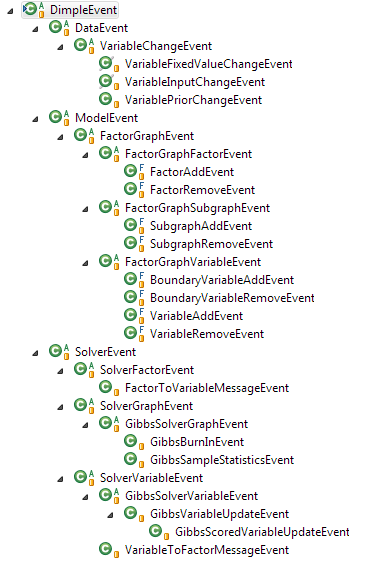
\includegraphics{images/EventHierarchy.png}
  \caption{Dimple event hierarchy}
  \label{fig:EventHierarchy}
\end{figure}

Dimple Events are organized hierarchically, and the current version of the full hierarchy is shown in Figure \ref{fig:EventHierarchy}. Note that any event types marked with an 'A' in the diagram are abstract super types and are used to organize the events by category. Actual event instances will belong to non-abstract types, which are for the most part leaf-nodes in the diagram. Events are subdivided into three categories:

\begin{itemize}
\item ModelEvent: includes changes to the structure of the model including adding and removing variables, factors and subgraphs. The concrete model event types are:
  \begin{itemize}
  \item FactorAddEvent and FactorRemoveEvent: raised when a factor is added or removed from the model.
  \item VariableAddEvent and VariableRemoveEvent: raised when a variable is added or removed from the model.
  \item SubgraphAddEvent and SubgraphRemoveEven: raised when a subgraph is added or removed from the model.
  \item BoundaryVariableAddEvent and BoundaryVariableRemoveEvent: raised when a boundary variable is added or removed.
  \end{itemize}
\item DataEvent: includes changes to data including changes to fixed values and inputs. The concrete data event types are:
  \begin{itemize}
  \item VariableFixedValueChangeEvent: raised when a fixed value is set or unset on a variable.
  \item VariableInputChangeEvent: raised when an input distribution is set or unset on a variable.
  \end{itemize}
\item SolverEvent: includes solver-specific events of interest that occur while running inference. The concrete event types are:
  \begin{itemize}
  \item FactorToVariableMessageEvent and VariableToFactorMessageEvent: raised when edge messages are updated in belief propagation solvers. Currently only the sumproduct and minsum solvers generate these messages.
  \item GibbsBurnInEvent: raised upon completion of random-restart and burn-in phase of Gibbs solver.
  \item GibbsSampleStatisticsEvent: raised after generation of one set of samples for the graph have been generated by the Gibbs solver. Contains statistics relevant to the sample.
  \item GibbsVariableUpdateEvent and GibbsScoredVariableUpdateEvent: raised when sample values are changed by the Gibbs solver. The two event types are the same except that the scored version adds information about the change in score induced by the sample update.
  \end{itemize}
\end{itemize}

Additional events may be added in future releases. New event types may also be added by developers who have extended Dimple with their own solvers or custom factors in Java.

\ifmatlab
When specifying event types in the MATLAB API, use the event type name in a string value:

\begin{figure}[H]
\begin{lstlisting}
logger = getEventLogger();
logger.log('FactorToVariableMessageEvent', fg);
\end{lstlisting}
\end{figure}

Unrecognized event types will result in an exception.

Note that Dimple events are not MATLAB events and you cannot use MATLAB's event API to trigger or listen for Dimple events.
\fi

\ifjava
When specifying event types in the Java API, use the event class itself:

\begin{figure}[H]
\begin{lstlisting}
DimpleEventLogger logger = new DimpleEventLogger();
logger.log(FactorToVariableMessageEvent.class, fg);
\end{lstlisting}
\end{figure}
\fi

\FloatBarrier

\subsubsection{Event logging}

The easiest way to monitor events in Dimple is through an event logger. Given an event logger instance, you can configure it to log either to the console or to a text file, you can configure how verbose the output should be, and specify which events for which model objects should be logged.

\ifmatlab
Event loggers are instances of the EventLogger class. You may create an
instance using the constructor:

\begin{figure}[H]
\begin{lstlisting}
logger = EventLogger();
\end{lstlisting}
\end{figure}

or you may simply get the default global instance using the getEventLogger() function, which will create a new logger the first time it is invoked:

\begin{figure}[H]
\begin{lstlisting}
logger = getEventLogger();
\end{lstlisting}
\end{figure}
\fi

\ifjava
Event loggers are instances of the DimpleEventLogger class. You may create a new one using the constructor:

\begin{lstlisting}
DimpleEventLogger logger = new DimpleEventLogger();
\end{lstlisting}
\fi

Newly constructed loggers will output to standard error by default and will have a default verbosity of zero, which will produce the most terse output. You may configure the logger to change the verbosity level or to direct output to a different target. For example:

\begin{figure}[H]
\ifmatlab
\begin{lstlisting}
% Use more verbose log output.
logger.Verbosity = 2;

% Append output to a file in the working directory.
logger.open('event-logger.txt');

% ... or output to standard output
logger.open('stdout');
\end{lstlisting}
\fi

\ifjava
\begin{lstlisting}
// Use more verbose log output.
logger.verbosity(2);

// Append output to a file in the working directory.
logger.open(new File("event-logger.txt"));

// ... or output to standard output
logger.open(System.out);
\end{lstlisting}
\fi
\end{figure}

Usually a single logger will be sufficient, but you can create multiple logger objects that direct output to different targets.

To enable logging for a particular class of events on your model, use the log method with the event type of interest. If the event type is abstract (is annotated with the letter A in Figure \ref{fig:EventHierarchy}), then
all event subtypes will be logged. If the event type is not abstract, then
only that particular event type will be logged. In particular, if you specify SolverEvent on a graph using the Gibbs solver, you will see
GibbsScoredVariableUpdateEvent messages but if you specify
GibbsVariableUpdateEvent you will get only messages for that specific
class and will not get scored messages.

\begin{figure}[H]
\ifmatlab
\begin{lstlisting}
% Log all solver events for given model.
logger.log('SolverEvent', model);

% Log unscored Gibbs update messages
logger.log('GibbsVariableUpdateEvent', model);

% Log variable to factor messages for a single variable
logger.log('VariableToFactorMessageEvent', x);
\end{lstlisting}
\fi

\ifjava
\begin{lstlisting}
// Log all solver events for given model.
logger.log(SolverEvent.class, model);

// Log unscored Gibbs update messages
logger.log(GibbsVariableUpdateEvent.class, model);

// Log variable to factor messages for a single variable
logger.log(VariableToFactorMessageEvent.class, x);
\end{lstlisting}
\fi
\end{figure}

You may remove previously created log registration either by
using the unlog method to remove individual entries or the clear
method to remove all entries. When using unlog, the arguments must
match the original arguments passed to log. (Note that setting the verbosity to a negative value or closing the output will also turn off logging it will not prevent Dimple from creating the underlying events, so make sure to use the clear() method when you are done with logging if you do not want to slow down inference.)

\begin{figure}[H]
\ifmatlab
\begin{lstlisting}
% Disable a previous log registration
logger.log('SolverEvent', model);

% Disable all logging
logger.clear();
\end{lstlisting}
\fi

\ifjava
\begin{lstlisting}
// Disable a previous log registration
logger.log(SolverEvent.class, model);

// Disable all logging
logger.clear();
\end{lstlisting}
\fi
\end{figure}

When using logging, it is usually very helpful to give the variables, factors and
subgraphs unique, easy to read, names. This will make your log output much easier to understand.

\subsubsection{Advanced event handling}

\ifmatlab
The MATLAB API does not support handling Dimple events outside of the EventLogger
class. More advanced uses cases may be implemented using the Java API. See the Java version of this manual for details.
\fi

\ifjava
The DimpleEventLogger class provides an easy way to monitor changes when
running inference in Dimple, but it does not let you interact directly with 
the event objects or take actions other than simple logging. A much wider range of
options is available by using the event handler and listener framework upon which the
logger is based. This is described in more detail in the next sections.

\subsubsection{Event listeners}
An object of type DimpleEventListener may be attached to the root FactorGraph of the model by the FactorGraph.setEventListener method and will be used to dispatch all events generated by the model and its associated data and solver layers. If there is no listener on the root graph, then no events should be generated. By default there is no listener for newly created graphs. When creating a listener, you can either create a new instance or use the global default instance that is lazily created by DimpleEventListener.getDefault(). Note that the DimpleEventLogger automatically adds the default listener to the root graph of models that don't already have a listener when a new log specification is registered for a child of the graph, but you will need to do this explicitly if you are not using that class.

Once a listener has been associated with the graph, then one or more handlers may be registered to handle events on the graph. The registration must specify the base class of the type of event to be handled and the root object on which events will be raised. It will be easiest to register for events at the root graph, but it may sometimes be desirable to set up handlers for specific variables, factors or subgraphs. For instance, to register handlers for various belief propagation messages on a graph, you could write: 

\begin{figure}[H]
\begin{lstlisting}
DimpleEventListener listener = DimpleEventListener.getDefault();
fg.setEventListener(listener);
listener.register(factorMessageHandler,
    FactorToVariableMessageEvent.class, fg);
listener.register(variableMessageHandler,
    VariableToFactorMessageEvent.class, fg);
\end{lstlisting}
\end{figure}

Handlers can be removed by one of the various unregister methods on the listener; see the Java API doc for that class for details. Changes to event registration or the value of the root listener are not guaranteed to take effect until the next time the affected objects have been initialized or the IDimpleEventSource.notifyListenerChanged() method has been invoked on the object that generates the event. This is important for model events in particular since model changes typically occur prior to initialization. 

\subsubsection{Event handlers}
Dimple event handlers are objects that implement the IDimpleEventHandler interface. In practice most handlers should simply extend the abstract base class DimpleEventHandler. For example, here is a simple handler class that simply prints events out to the console with a verbosity of one: 

\begin{figure}[H]
\begin{lstlisting}
public class EventPrinter extends DimpleEventHandler<DimpleEvent>
{
    public void handleEvent(DimpleEvent event)
    {
        event.println(System.out, 1);
    }
}
\end{lstlisting}
\end{figure}

Handler classes that are specific to a particular event subclass can be parameterized appropriately to avoid the need for downcasts. For example, here is a simple handler that keeps a running total of the total graph score during Gibbs sampling based on sample score differences:

\begin{figure}[H] 
\begin{lstlisting}
public class RunningScoreHandler extends DimpleEventHandler<GibbsScoredVariableUpdateEvent>
{
    public double score;

    RunningScoreHandler(double startingScore)
    {
        score = startingScore;
    }

    public void handleEvent(GibbsScoredVariableUpdateEvent event)
    {
        score += event.getScoreDifference();
    }
}
\end{lstlisting}
\end{figure}

\fi
\subsection{List of Built-in Factors}
\label{sec:builtInFactors}

The following table lists the current set of built-in Dimple factors.  For each, the name is given, followed by the set of variables that would be connected to the factor, followed by any constructor arguments.  Optional variables and constructor arguments are in brackets.  And an arbitrary length list or vector of variables is followed by ellipses.  The allowed set of variable data-types for each variable is given in parentheses (B~=~Bit, D~=~Discrete, R~=~Real, C~=~Complex).

\begin{longtable} {l p{2.2cm} p{2cm} p{7cm}}
Name & Variables & Constructor & Description \\
\hline
\endhead
%
Abs & out(D,R) \newline in(D,R) & [smoothing] & Deterministic absolute value function, where out = abs(in).  An optional smoothing value may be specified as a constructor argument\footnote{\label{ftn:smoothing}If smoothing is enabled, the factor function becomes $e^{-(\textrm{out} - F(\textrm{in}))^2/\textrm{smoothing}}$ (making it non-deterministic) instead of $\delta(\textrm{out} - F(\textrm{in}))$, where $F$ is the deterministic function associated with this factor.  This is useful for solvers that do not work well with deterministic real-valued factors, such as particle BP, particularly when tempering is used.}.\\
%
ACos & out(D,R) \newline in(D,R) & [smoothing] & Deterministic arc-cosine function, where out = acos(in). An optional smoothing value may be specified as a constructor argument$^{\ref{ftn:smoothing}}$. \\
%
AdditiveNoise & out(R) \newline in(B,D,R) & $\sigma$ & Add Gaussian noise with a known standard deviation, $\sigma$, specified in constructor. \\
%
And & out(B) \newline in...(B) & - & Deterministic logical AND function, where out = AND(in...). \\
%
ASin & out(D,R) \newline in(D,R) & [smoothing] & Deterministic arc-sine function, where out = asin(in). An optional smoothing value may be specified as a constructor argument$^{\ref{ftn:smoothing}}$. \\
%
ATan & out(D,R) \newline in(D,R) & [smoothing] & Deterministic arc-tangent function, where out = atan(in). An optional smoothing value may be specified as a constructor argument$^{\ref{ftn:smoothing}}$. \\
%
Beta & [$\alpha$](R) \newline [$\beta$](R) \newline value...(R) & [$\alpha$] \newline [$\beta$] & Beta distribution. There can be any number of value variables, all associated with the same parameter values.  Parameters $\alpha$ and $\beta$ can be variables, or if both are constant they can be specified in the constructor. \\
%
Categorical & $\alpha$...(R)  \newline x...(D) & N & Categorical distribution, $p(x | \alpha)$, where $\alpha$ is a vector of parameter variables and x is a vector of discrete variables.  The number of elements in $\alpha$ and the domain size of x must equal the value of the constructor argument, N.  There can be any number of x variables, all associated with the same parameter values.  \newline
The $\alpha$ parameters are represented as energy values, that is, $\alpha = -\log(\rho)$, where $\rho$ are unnormalized probabilities. The conjugate prior for this representation is such that each entry of $\alpha$ is independently distributed according to a negative exp-Gamma distribution, all with a common $\beta$ parameter (it is not necessary to use the conjugate prior, but in some cases there may be a benefit).  \newline
In the current implementation, the domain of the x variable must be zero-based contiguous integers, $0...N-1$ (this limitation may be lifted in a future version). \\
%
ComplexConjugate & out(C) \newline in(C,R) & [smoothing] & Deterministic complex conjugate function, where out = in$^{*}$. An optional smoothing value may be specified as a constructor argument$^{\ref{ftn:smoothing}}$. \\
%
ComplexDivide & quotient(C) \newline dividend(C,R) \newline divisor(C,R) & [smoothing] & Deterministic complex divide function, where $\mathrm{quotient} = \frac{\mathrm{dividend}}{\mathrm{divisor}}$. An optional smoothing value may be specified as a constructor argument$^{\ref{ftn:smoothing}}$. \\
%
ComplexExp & out(C) \newline in(C,R) & [smoothing] & Deterministic complex exponentiation function, where out = exp(in). An optional smoothing value may be specified as a constructor argument$^{\ref{ftn:smoothing}}$. \\
%
ComplexNegate & out(C) \newline in(C,R) & [smoothing] & Deterministic complex negation function, where out = -in. An optional smoothing value may be specified as a constructor argument$^{\ref{ftn:smoothing}}$. \\
%
ComplexProduct & out(C) \newline in...(C,R) & [smoothing] & Deterministic complex product function, where $\mathrm{out} = \prod \mathrm{in}$. An optional smoothing value may be specified as a constructor argument$^{\ref{ftn:smoothing}}$. \\
%
ComplexSubtract & out(C) \newline posIn(C,R) \newline negIn...(C,R) & [smoothing] & Deterministic complex subtraction function, where $\mathrm{out} = \mathrm{posIn} - \sum \mathrm{negIn}$. An optional smoothing value may be specified as a constructor argument$^{\ref{ftn:smoothing}}$. \\
%
ComplexSum & out(C) \newline in...(C,R) & [smoothing] & Deterministic complex summation function, where $\mathrm{out} = \sum \mathrm{in}$. An optional smoothing value may be specified as a constructor argument$^{\ref{ftn:smoothing}}$. \\
%%
%% Primarily for testing, need not be listed here.
%ConstantPower & out(D,R) \newline base(D,R) & power \newline [smoothing] & Deterministic power function, with a constant power. The power value is specified in the constructor. An optional smoothing value may be specified as a constructor argument$^{\ref{ftn:smoothing}}$. \\
%%
%% Primarily for testing, need not be listed here.
%ConstantProduct & out(D,R) \newline in(D,R) & constant \newline [smoothing] &  Deterministic product function, multiplying the input times a constant value.  The constant value is specified in the constructor. An optional smoothing value may be specified as a constructor argument$^{\ref{ftn:smoothing}}$. \\
%
Cos & out(D,R) \newline in(D,R) & [smoothing] & Deterministic cosine function, where out = cos(in). An optional smoothing value may be specified as a constructor argument$^{\ref{ftn:smoothing}}$. \\
%
Cosh & out(D,R) \newline in(D,R) & [smoothing] & Deterministic hyperbolic-cosine function, where out = cosh(in). An optional smoothing value may be specified as a constructor argument$^{\ref{ftn:smoothing}}$. \\
%
DiscreteTransition & x(D) \newline y(D) \newline A(R) & $N_{x}, N_{y} | \newline N$ & 
Parameterized discrete transition factor, $p(y | x, A)$, where x and y are discrete variables, and $A$ is a matrix of transition probabilities. The transition matrix is organized such that columns correspond to the output distribution for each input state. That is, the transition matrix multiplies on the left. The number of columns in A and the domain size of x must equal the value of the constructor argument, $N_{x}$ and the number of rows in A and the domain size of y must equal the value of the constructor argument $N_{y}$.  If $N_{x}$ and $N_{y}$ are equal, a single constructor argument, $N$, may be used.  \newline
The elements of the matrix A are represented as energy values, that is, $A_{i,j} = -\log(\rho_{i,j})$, where $\rho$ is an unnormalized transition probability matrix.  The conjugate prior for this representation is such that each entry of A is independently distributed according to a negative exp-Gamma distribution, all with a common $\beta$ parameter (it is not necessary to use the conjugate prior, but in some cases there may be a benefit).  \newline
In the current implementation, the domain of the x variable must be zero-based contiguous integers, $0...N-1$ (this limitation may be lifted in a future version). \\
%
Divide & quotient(D,R) \newline dividend(D,R) \newline divisor(D,R) & [smoothing] & Deterministic divide function, where $\mathrm{quotient} = \frac{\mathrm{dividend}}{\mathrm{divisor}}$. An optional smoothing value may be specified as a constructor argument$^{\ref{ftn:smoothing}}$. \\
%
Equality & value...(B,D,R) & [smoothing] & Deterministic equality constraint.  An optional smoothing value may be specified as a constructor argument$^{\ref{ftn:smoothing}}$. \\
%
Equals & out(B) \newline in...(B,D,R) & - & Deterministic equals function, where out~=~(in(1)~==~in(2)~== ... ). \\
%
Exp & out(D,R) \newline in(D,R) & [smoothing] & Deterministic exponentiation function, where out = exp(in). An optional smoothing value may be specified as a constructor argument$^{\ref{ftn:smoothing}}$. \\
%
Gamma & [$\alpha$](R) \newline [$\beta$](R) \newline value...(R) & [$\alpha$] \newline [$\beta$] & Gamma distribution. There can be any number of value variables, all associated with the same parameter values.  Parameters $\alpha$ and $\beta$ can be variables, or if both are constant they can be specified in the constructor. \\
%
GreaterThan & out(B) \newline in1(B,D,R) \newline in2(B,D,R) & - & Deterministic greater-than function, where out = in1 $>$ in2.  \\
%
InverseGamma & [$\alpha$](R) \newline [$\beta$](R) \newline value...(R) & [$\alpha$] \newline [$\beta$] & Inverse Gamma distribution. There can be any number of value variables, all associated with the same parameter values.  Parameters $\alpha$ and $\beta$ can be variables, or if both are constant they can be specified in the constructor. \\
%
LessThan & out(B) \newline in1(B,D,R) \newline in2(B,D,R) & - & Deterministic greater-than function, where out = in1 $<$ in2.  \\
%
LinearEquation & out(D,R) \newline in(B,D,R) & constants \newline [smoothing] & Deterministic linear equation, multiplying an input vector by a constant vector. The constant vector is specified in the constructor.  The number of \emph{in} variables must equal the length of the constant vector. An optional smoothing value may be specified as a constructor argument\textsuperscript{\ref{ftn:smoothing}}. \\
%
Log & out(D,R) \newline in(D,R) & [smoothing] & Deterministic natural log function, where out = log(in). An optional smoothing value may be specified as a constructor argument$^{\ref{ftn:smoothing}}$. \\
%
LogNormal & [$\mu$](R) \newline [$\tau$](R) \newline value...(R) & [$\mu$] \newline [$\tau$] & Log-normal distribution. There can be any number of value variables, all associated with the same parameter values.  Parameters $\mu$ (mean) and $\tau = \frac{1}{\sigma^{2}}$ (precision) can be variables, or if both are constant then fixed parameters can be specified in the constructor. \\
%
MatrixVectorProduct & y(D,R) \newline M(D,R) \newline x(D,R) & $N_{x}$ \newline $N_{y}$ \newline [smoothing] & Deterministic matrix-vector product function, $y = Mx$, where $x$ and $y$ are vectors and $M$ is a matrix. Constructor arguments, $N_{x}$ and $N_{y}$, specify the input and output vector lengths, respectively. The matrix dimension is $N_{y} \times N_{x}$. An optional smoothing value may be specified as a constructor argument$^{\ref{ftn:smoothing}}$. \\
%%
%% Primarily for testing, need not be listed here.
%MixedNormal & value(R) \newline control(B) & $\mu_{0} \newline \tau_{0} \newline \mu_{1} \newline \tau_{1}$ & Simple mixture of two fixed-parameter Normal distributions. The choice of distribution parameters (0 vs. 1) is a function of the control bit. \\
%
Negate & out(D,R) \newline in(D,R) & [smoothing] & Deterministic negation function, where out = -in. An optional smoothing value may be specified as a constructor argument$^{\ref{ftn:smoothing}}$. \\
%
NegativeExpGamma & [$\alpha$](R) \newline [$\beta$](R) \newline value...(R) & [$\alpha$] \newline [$\beta$] & Negative exp-Gamma distribution, which is a distribution over a variable whose negative exponential is Gamma distributed. That is, this is the negative log of a Gamma distributed variable. There can be any number of value variables, all associated with the same parameter values.  Parameters $\alpha$ and $\beta$ can be variables, or if both are constant they can be specified in the constructor, and correspond to the parameters of the underlying Gamma distribution. \\
%
Normal & [$\mu$](R) \newline [$\tau$](R) \newline value...(R) & [$\mu$] \newline [$\tau$] & Normal distribution. There can be any number of value variables, all associated with the same parameter values.  Parameters $\mu$ (mean) and $\tau = \frac{1}{\sigma^{2}}$ (precision) can be variables, or if both are constant then fixed parameters can be specified in the constructor. \\
%
Not & out(B) \newline in(B) & - & Deterministic logical NOT of function, where out = ~in. \\
%
NotEquals & out(B) \newline in...(B,D,R) & - & Deterministic not-equals function, where out~=~$\sim$(in(1)~==~in(2)~== ... ). \\
%
Or & out(B) \newline in...(B) & - & Deterministic logical OR function, where out = OR(in...). \\
%
Power & out(D,R) \newline base(D,R) \newline power(D,R) & [smoothing] & Deterministic power function, where out~=~base~$^{\mathrm{power}}$. An optional smoothing value may be specified as a constructor argument$^{\ref{ftn:smoothing}}$. \\
%
Product & out(D,R) \newline in...(B,D,R) & [smoothing] & Deterministic product function, where $\mathrm{out} = \prod \mathrm{in}$. An optional smoothing value may be specified as a constructor argument$^{\ref{ftn:smoothing}}$. \\
%
Rayleigh & [$\sigma$](R) \newline value...(R) & [$\sigma$] & Rayleigh distribution. There can be any number of value variables, all associated with the same parameter value.  Parameter $\sigma$ can be a variable, or if constant, can be specified in the constructor. \\
%
Sin & out(D,R) \newline in(D,R) & [smoothing] & Deterministic sine function, where out = sin(in). An optional smoothing value may be specified as a constructor argument$^{\ref{ftn:smoothing}}$. \\
%
Sinh & out(D,R) \newline in(D,R) & [smoothing] & Deterministic hyperbolic-sine function, where out = sinh(in). An optional smoothing value may be specified as a constructor argument$^{\ref{ftn:smoothing}}$. \\
%
Sqrt & out(D,R) \newline in(D,R) & [smoothing] & Deterministic square root function, where out = sqrt(in). An optional smoothing value may be specified as a constructor argument$^{\ref{ftn:smoothing}}$. \\
%
Square & out(D,R) \newline in(D,R) & [smoothing] & Deterministic square function, where out = in$^{2}$. An optional smoothing value may be specified as a constructor argument$^{\ref{ftn:smoothing}}$. \\
%
Subtract & out(D,R) \newline posIn(B,D,R) \newline negIn...(B,D,R) & [smoothing] & Deterministic subtraction function, where $\mathrm{out} = \mathrm{posIn} - \sum \mathrm{negIn}$. An optional smoothing value may be specified as a constructor argument$^{\ref{ftn:smoothing}}$. \\
%
Sum & out(D,R) \newline in...(B,D,R) & [smoothing] & Deterministic summation function, where $\mathrm{out} = \sum \mathrm{in}$. An optional smoothing value may be specified as a constructor argument$^{\ref{ftn:smoothing}}$. \\
%
Tan & out(D,R) \newline in(D,R) & [smoothing] & Deterministic tangent function, where out = tan(in). An optional smoothing value may be specified as a constructor argument$^{\ref{ftn:smoothing}}$. \\
%
Tanh & out(D,R) \newline in(D,R) & [smoothing] & Deterministic hyperbolic-tangent function, where out = tanh(in). An optional smoothing value may be specified as a constructor argument$^{\ref{ftn:smoothing}}$. \\
%
VonMises & [$\mu$](R) \newline [$\tau$](R) \newline value...(R) & [$\mu$] \newline [$\tau$] & Von Mises distribution. There can be any number of value variables, all associated with the same parameter values.  Parameters $\mu$ (mean) and $\tau = \frac{1}{\sigma^{2}}$ (precision) can be variables, or if both are constant then fixed parameters can be specified in the constructor.  The distribution is non-zero for value variables in the range $-\pi$ to $\pi$. \\
%
Xor & out(B) \newline in...(B) & - & Deterministic logical XOR function, where out = XOR(in...). \\
%
\end{longtable}

\subsubsection{Solver-Specific Built-in Factors}
\label{sec:solverSpecificBuiltInFactors}

In addition to the built-in factors listed above, there are a set of solver-specific built-in factors, also referred to as ``custom factors.''  These factors may also be specified by name in the addFactor call (using either a quoted string or as a function handle).  These are summarized in the following table:

\begin{longtable} {l p{3cm} p{7cm}}
Name & Solver & Description \\
\hline
\endhead
%
FiniteFieldFactor & SumProduct\footnote{\label{ftn:fff} These may also be used for discrete variables with the Gaussian or particle BP solvers, which use the sum-product solver for discrete-only portions of the graph.}  & See section~\ref{sec:finiteFields} \\ 
FiniteFieldProjection & SumProduct$^{\ref{ftn:fff}}$ & See section~\ref{sec:finiteFields} \\ 
FiniteFieldAdd & SumProduct$^{\ref{ftn:fff}}$ & See section~\ref{sec:finiteFields} \\ 
FiniteFieldConstMult & SumProduct$^{\ref{ftn:fff}}$ & See section~\ref{sec:finiteFields} \\ 
FiniteFieldMult & SumProduct$^{\ref{ftn:fff}}$ & See section~\ref{sec:finiteFields} \\ 
CustomXor & MinSum & Same as the Xor factor described above, but with a significantly faster implementation. \\ 
\end{longtable}


\ifmatlab

\subsubsection{Factor Creation Utility Functions}

Dimple includes some helper functions to create other built-in factors using a similar syntax to the overloaded MATLAB functions described in section~\ref{sec:overloaded}.  As for other overloaded functions, above, Dimple automatically creates the factors as well as the output variable(s).  Such helper functions are defined for the following built-in distributions:

\begin{itemize}
\item Beta
\item Gamma
\item InverseGamma
\item NegativeExpGamma
\item Normal
\item LogNormal
\item VonMises
\item Rayleigh
\item Categorical
\end{itemize}

For each, the arguments are the parameters of the distribution.  For example:

\begin{lstlisting}
W = Gamma(alpha, beta);
X = Normal(mean, precision);
Y = Categorical(alphaVector);
Z = Rayleigh(sigma);
\end{lstlisting}


The parameters can be variables, constants, or some of each.

By default, calling one of these functions creates a single output variable, and the factor is added to the most-recently created graph. �But, optional arguments allow you to specify the dimensions of the array of output variables, or to specify the factor graph. �These arguments can be in either order after the parameters. �For example:

\begin{lstlisting}
W = Gamma(alpha, beta, altGraph);
X = Normal(mean, precision, [100, 1]);
Y = Categorical(alphaVector, [10, 10, 2], aGraph);
Z = Rayleigh(sigma, myGraph, size(somethingElse));
\end{lstlisting}


Dimple also includes some built-in helper functions to create structured graphs, combining smaller factors to form an efficient implementation of a larger subgraph.  Specifically, the following functions are provided:

\begin{itemize}
\item getNBitXorDef(n), where n is a positive integer. Returns a nestable graph and an array of n-Bit connector variables. Efficient tree implementation of the XORDelta function.
\item getVXOR(n), where n is a positive integer. Returns a nestable graph and an array of n-Bits connector variables. Constrains exactly one bit to be 1, and all others to be 0.
\end{itemize}

\fi



\ifmatlab
\subsection{List of Overloaded MATLAB Operators and Functions}
\label{sec:overloaded}

The following table lists the set of overloaded MATLAB operators that can be used to implicitly create factors.  The table shows the operator, the corresponding factor, the valid variable data types of the inputs and outputs (B = Bit, D = Discrete, or R = Real), and wether or not vectorized inputs are supported.

\begin{longtable} {l p{3cm} p{1cm} p{1cm} p{1cm} l p{4cm}}
Operator & Factor & Out & In1 & In2 & Vectorized & Description \\
\hline
\endhead
%
$\&$ & And & B & B & B & \checkmark & Logical AND \\
$|$ & Or & B & B & B & \checkmark & Logical OR \\
xor() & Xor & B & B & B & \checkmark & Logical XOR \\
$\sim$ & Not & B & B & - & \checkmark & Logical NOT \\
$+$ & Sum & D,R\footnote{\label{ftn:outReal}If either input is Real, then the output is Real} & D,R & D,R & \checkmark & Plus \\
$-$ & Subtract & D,R\textsuperscript{\ref{ftn:outReal}} & D,R & D,R & \checkmark & Minus \\
$-$ & Negate & D,R\textsuperscript{\ref{ftn:outReal}} & D,R & - & \checkmark & Unary minus \\
$*$ & Product \newline MatrixVectorProduct & D,R\textsuperscript{\ref{ftn:outReal}} & D,R & D,R & \checkmark\footnote{One of the inputs may be a vector as long as the other is a scalar.} & Scalar multiply, or matrix-vector multiply\footnote{If one input is a vector and the other is a matrix of appropriate dimension, then the MatrixVectorProduct factor will be used.  Otherwise the Product factor will be used.} \\
$.*$ & Product & D,R\textsuperscript{\ref{ftn:outReal}} & D,R & D,R & \checkmark & Point-wise multiply \\
$/$ & Divide & D,R\textsuperscript{\ref{ftn:outReal}} & D,R & D,R & \checkmark\footnote{The dividend may be a vector as long as the divisor is a scalar.} & Scalar divide \\
$./$ & Divide & D,R\textsuperscript{\ref{ftn:outReal}} & D,R & D,R & \checkmark & Point-wise divide \\
$\wedge$ & Power & D,R\textsuperscript{\ref{ftn:outReal}} & D,R & D,R & \checkmark\footnote{The base may be a vector as long as the exponent is a scalar.} & Scalar power \\
$.\wedge$ & Power & D,R\textsuperscript{\ref{ftn:outReal}} & D,R & D,R & \checkmark & Point-wise power \\
$<$ & LessThan & B & D,R & D,R & \checkmark & Less than \\
$>$ & GreaterThan & B & D,R & D,R & \checkmark & Greater than \\
$<=$ & GreaterThan\footnote{Uses GreaterThan factor, reversing the order.} & B & D,R & D,R & \checkmark & Less than or equal to \\
$>=$ & LessThan\footnote{Uses LessThan factor, reversing the order.} & B & D,R & D,R & \checkmark & Greater than or equal to \\
Equals() & Equals & B & B,D,R & B,D,R\footnote{\label{ftn:equals}This function is not limited to two inputs, but can take an arbitrary number of inputs} & \checkmark & Equals\footnote{Equivalent to the $==$ operator, but the $==$ operator is not overloaded for this purpose so that it can instead be used to determine whether or not two variables reference the same Dimple variable.} \\
NotEquals() & NotEquals & B & B,D,R & B,D,R$^{\ref{ftn:equals}}$ & \checkmark & Not equals\footnote{Equivalent to the $\sim=$ operator, but the $\sim=$ operator is not overloaded for this purpose so that it can instead be used to determine whether or not two variables reference the same Dimple variable.} \\
mod() & - & D  & D & D & \checkmark & Modulo function\footnote{Currently, the mod() operator supports discrete variables only, and it uses the MATLAB definition of mod on negative numbers.  This may be subject to change in future versions.} \\
abs() & Abs & D,R\textsuperscript{\ref{ftn:outReal}} & D,R & - & \checkmark & Absolute value \\
sqrt() & Sqrt & R & R & - & \checkmark & Square root \\
log() & Log & R & R & - & \checkmark & Natural log \\
exp() & Exp & R & R & - & \checkmark & Exponential function \\
sin() & Sin & R & R & - & \checkmark & Sine \\
cos() & Cos & R & R & - & \checkmark & Cosine \\
tan() & Tan & R & R & - & \checkmark & Tangent \\
asin() & ASin & R & R & - & \checkmark & Arc-sine \\
acos() & ACos & R & R & - & \checkmark & Arc-cosine \\
atan() & ATan & R & R & - & \checkmark & Arc-tangent \\
sinh() & Sinh & R & R & - & \checkmark & Hyperbolic sine \\
cosh() & Cosh & R & R & - & \checkmark & Hyperbolic cosine \\
tanh() & Tanh & R & R & - & \checkmark & Hyperbolic tangent \\
\end{longtable}




\fi

\subsection{Other Top Level Functions}

\subsubsection{setSolver}

\begin{lstlisting}
setSolver('SolverName');
\end{lstlisting}

This function changes the default solver to the solver designated by the argument, which is a string indicating the name of the solver (see section~\ref{sec:FactorGraph.Solver} for the list of valid solver names, and section~\ref{sec:SolversAPI} for a description of each solver).  The solver name is case insensitive.


%\para{getSolverNames}
%
%\begin{lstlisting}
%getSolverNames()
%\end{lstlisting}
%
%
%\para{registerSolver}
%
%\begin{lstlisting}
%registerSolver(solverName,solverConstructor);
%\end{lstlisting}
%
%
%\para{unregisterSolver}
%
%\begin{lstlisting}
%unregisterSolver(solverName);
%\end{lstlisting}
%



